\section{Desempeño para distintos conjuntos de predictores}

Se analizó el rendimiento de la red neuronal para el pronóstico de precipitación para la región específica de Bocacosta, mediante las métricas de validación en el entrenamiento. Comparando cada uno de los conjuntos de predictores numerados en la subsección \ref{subsec:fuentes_de_datos}, con el objetivo de encontrar la mejor combinación posible para un adecuado pronóstico. Los resultados fueron los siguientes:
\begin{figure}[H]
	\centering
	
\includegraphics[width=13.0 cm]{Informe/resultados/comparacion_combinaciones.png}
	\caption{Comparación de métricas para distintos predictores}
	\label{fig:comparación_combinaciones}
\end{figure}

Así, la combinación 4 resultó ser claramente superior, presentando los errores MAE y RMSE más bajos, la correlación de Pearson, $R^2$ y NSE más altos, y uno de los índices de Kling-Gupta más altos de entre todos los predictores. Por esta razón, se entrenó el modelo con esta combinación para hacer el análisis de pronósticos de las secciones posteriores.

\section{Comparación con la precipitación real del año 2025 y los pronósticos de NextGen}

Se utilizó el modelo entrenado hasta diciembre de 2025 para pronosticar todos los meses del 2025, utilizando por tanto, los predictores de SST, TP; RMM1 y RMM2 de las MJO de treinta y un días previos al mes objetivo.

A continuación se presentan las estadísticas de error para los dos métodos (LSTM y NextGen) frente a las observaciones ENACTS para la región de Bocacosta durante el año 2025. Los valores corresponden a la misma partición temporal y espacial utilizada para el modelo LSTM.

\subsection*{Estadísticas globales y métricas mensuales}


\begin{figure}[H]
	\centering
	\begin{minipage}[t]{0.49\textwidth}
		\centering
		\scriptsize
		\begin{verbatim}
			Estadísticas globales LSTM
			RMSE                      = 102.5486
			MAE                       = 73.2204
			Bias (media)              = 47.2225
			% Bias                    = 20.17 %
			Std(error)                = 91.0288
			R^2                       = 0.7440
			Pearson r                 = 0.9166  (p=0.00e+00)
			Spearman rho              = 0.9122  (p=0.00e+00)
			Nash-Sutcliffe            = 0.7440
			Kling-Gupta (KGE)         = 0.7503
			
			Métricas por mes
			Mes    RMSE     MAE    Bias      r    KGE
			Ene  11.386   8.911   8.718  0.684  -0.269
			Feb  16.979  13.451  11.283 -0.033  -1.155
			Mar  54.753  44.010 -41.109  0.333   0.036
			Abr 118.727 108.897 108.897  0.730   0.011
			May 134.083 103.586  96.636  0.588   0.468
			Jun  73.831  59.520 -17.928  0.788   0.653
			Jul  65.896  52.331  -2.018  0.659   0.649
			Ago  71.430  58.784  41.050  0.848   0.703
			Sep 222.730 211.110 211.110  0.706   0.350
			Oct 135.631 117.971 114.210  0.722   0.570
			Nov  70.323  64.818  64.154  0.891   0.205
			Dic  53.467  35.258 -28.333 -0.246  -0.514
		\end{verbatim}
		\normalsize
	\end{minipage}
	\hfill
	\begin{minipage}[t]{0.49\textwidth}
		\centering
		\scriptsize
		\begin{verbatim}
			Estadísticas globales NextGen
			RMSE                      = 114.1463
			MAE                       = 77.9481
			Bias (media)              = 22.2838
			% Bias                    = 9.18 %
			Std(error)                = 111.9500
			R^2                       = 0.6931
			Pearson r                 = 0.8719  (p=0.00e+00)
			Spearman rho              = 0.8906  (p=0.00e+00)
			Nash-Sutcliffe            = 0.6931
			Kling-Gupta (KGE)         = 0.8094
			
			Métricas por mes
			Mes    RMSE     MAE    Bias      r    KGE
			Ene   6.297   4.744  -0.273 -0.076  -0.133
			Feb  12.914  11.171  11.081  0.544  -0.746
			Mar  50.241  37.716 -33.640  0.315   0.075
			Abr  47.790  36.629 -15.325  0.675   0.389
			May 118.062  96.606  78.933  0.640   0.565
			Jun 152.780 124.855 -80.979  0.321   0.307
			Jul 109.425  96.481  -1.718  0.356   0.194
			Ago  95.376  80.341 -49.203  0.675   0.658
			Sep 232.592 186.866 185.541  0.451  -0.232
			Oct 161.591 133.342 119.563  0.616   0.309
			Nov  97.153  86.908  77.540  0.454  -0.036
			Dic  57.773  39.718 -24.114 -0.322  -0.496
		\end{verbatim}
		\normalsize
	\end{minipage}
\end{figure}


\subsection*{Métricas mensuales medias}

\begin{figure}[H]
	\centering
	\begin{subfigure}[b]{0.48\textwidth}
		\centering
		\includegraphics[height=4.7 cm]{Informe/resultados/BocacostaLSTM/com.metricas.png}
		\subcaption{LSTM}
	\end{subfigure}
	\hfill
	\begin{subfigure}[b]{0.48\textwidth}
		\centering
		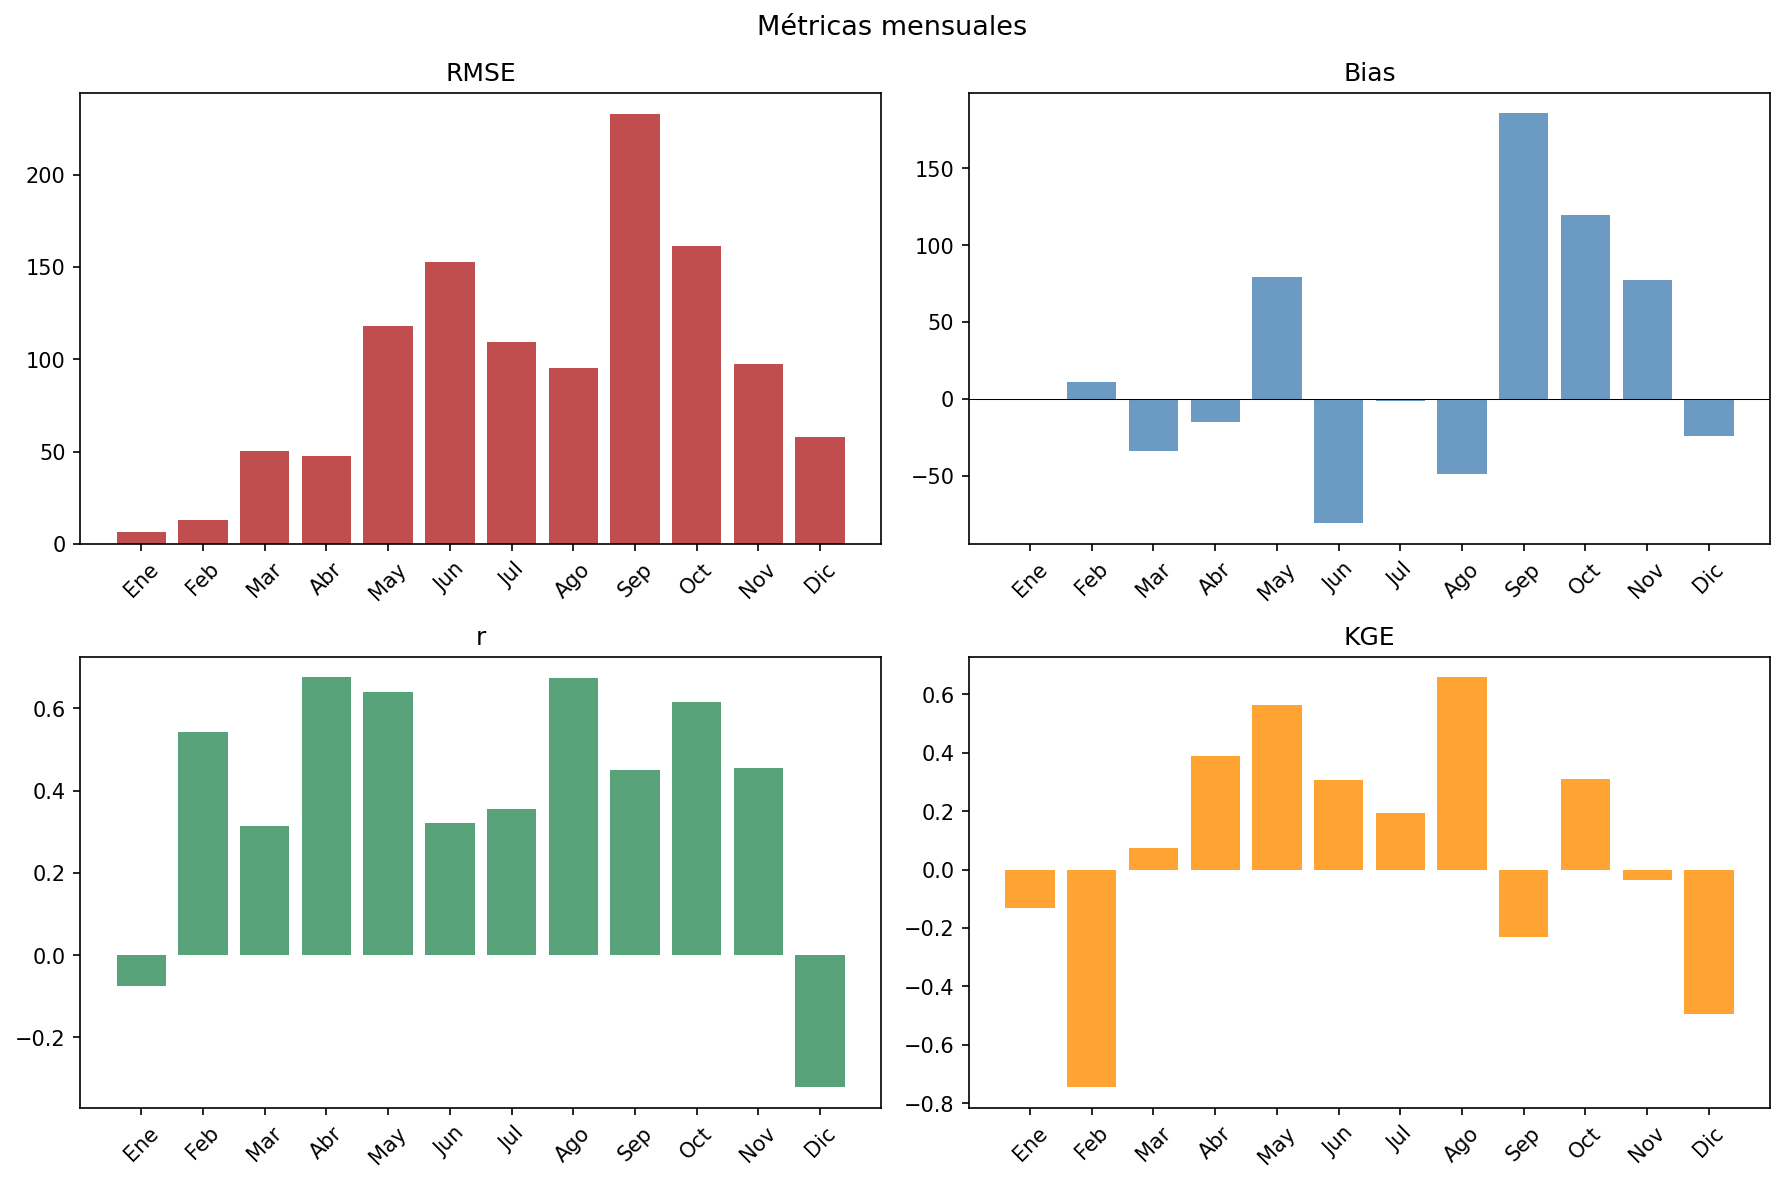
\includegraphics[height=4.7 cm]{Informe/resultados/BocacostaNextGen/com.metricas.png}
		\subcaption{NextGen}
	\end{subfigure}
	\caption{RMSE, sesgo medio, correlación de Pearson y coeficiente de Kling-Gupta mensuales medios para los datos de validación del entrenamiento en la región de Bocacosta.}
	\label{fig:metricas_comparadas}
\end{figure}

\subsection*{Ciclo anual medio de precipitación}

\begin{figure}[H]
	\centering
	\begin{subfigure}[b]{0.48\textwidth}
		\centering
		\includegraphics[height=4.7 cm]{Informe/resultados/BocacostaLSTM/com.cicloanual.png}
		\subcaption{LSTM}
	\end{subfigure}
	\hfill
	\begin{subfigure}[b]{0.48\textwidth}
		\centering
		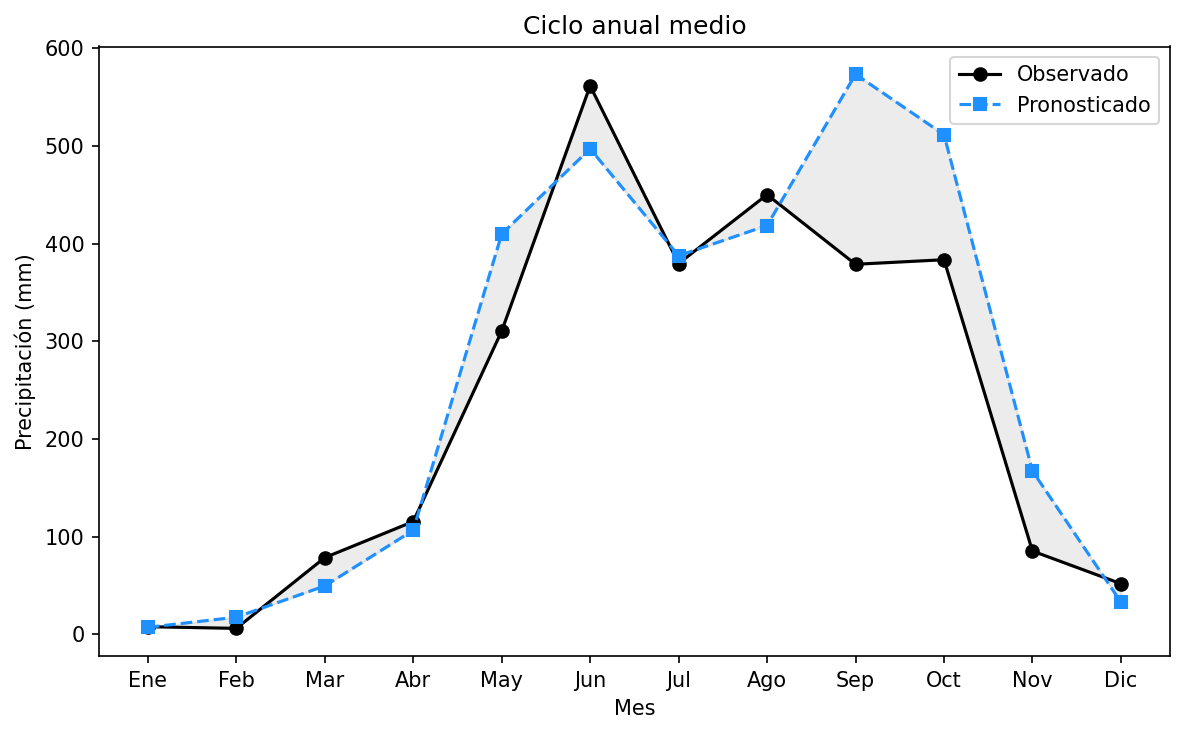
\includegraphics[height=4.7 cm]{Informe/resultados/BocacostaNextGen/com.cicloanual.png}
		\subcaption{NextGen}
	\end{subfigure}
	\caption{Precipitación media mensual para los datos de validación del entrenamiento en la región de Bocacosta.}
	\label{fig:cicloanual_comparado}
\end{figure}

Se presentan a continuación los pronósticos de la red neuronal y NextGen para todo el año 2025, y los datos observados de precipitación acumulada dada por el registro de datos de ENACTS. 

A continuación se presentan los mapas de precipitación para cada mes, ordenados en tres paneles, arriba a la izquierda: pronóstico LSTM; arriba a la derecha:  pronóstico NextGen; abajo: observaciones de ENACTS.

\begin{figure}[!htbp]
	\centering
	
	% ==================================================
	% ENERO
	% ==================================================
	
	\textbf{Enero 2025}
	
	\vspace{0.2em}
	
	\begin{subfigure}[b]{0.45\textwidth}
		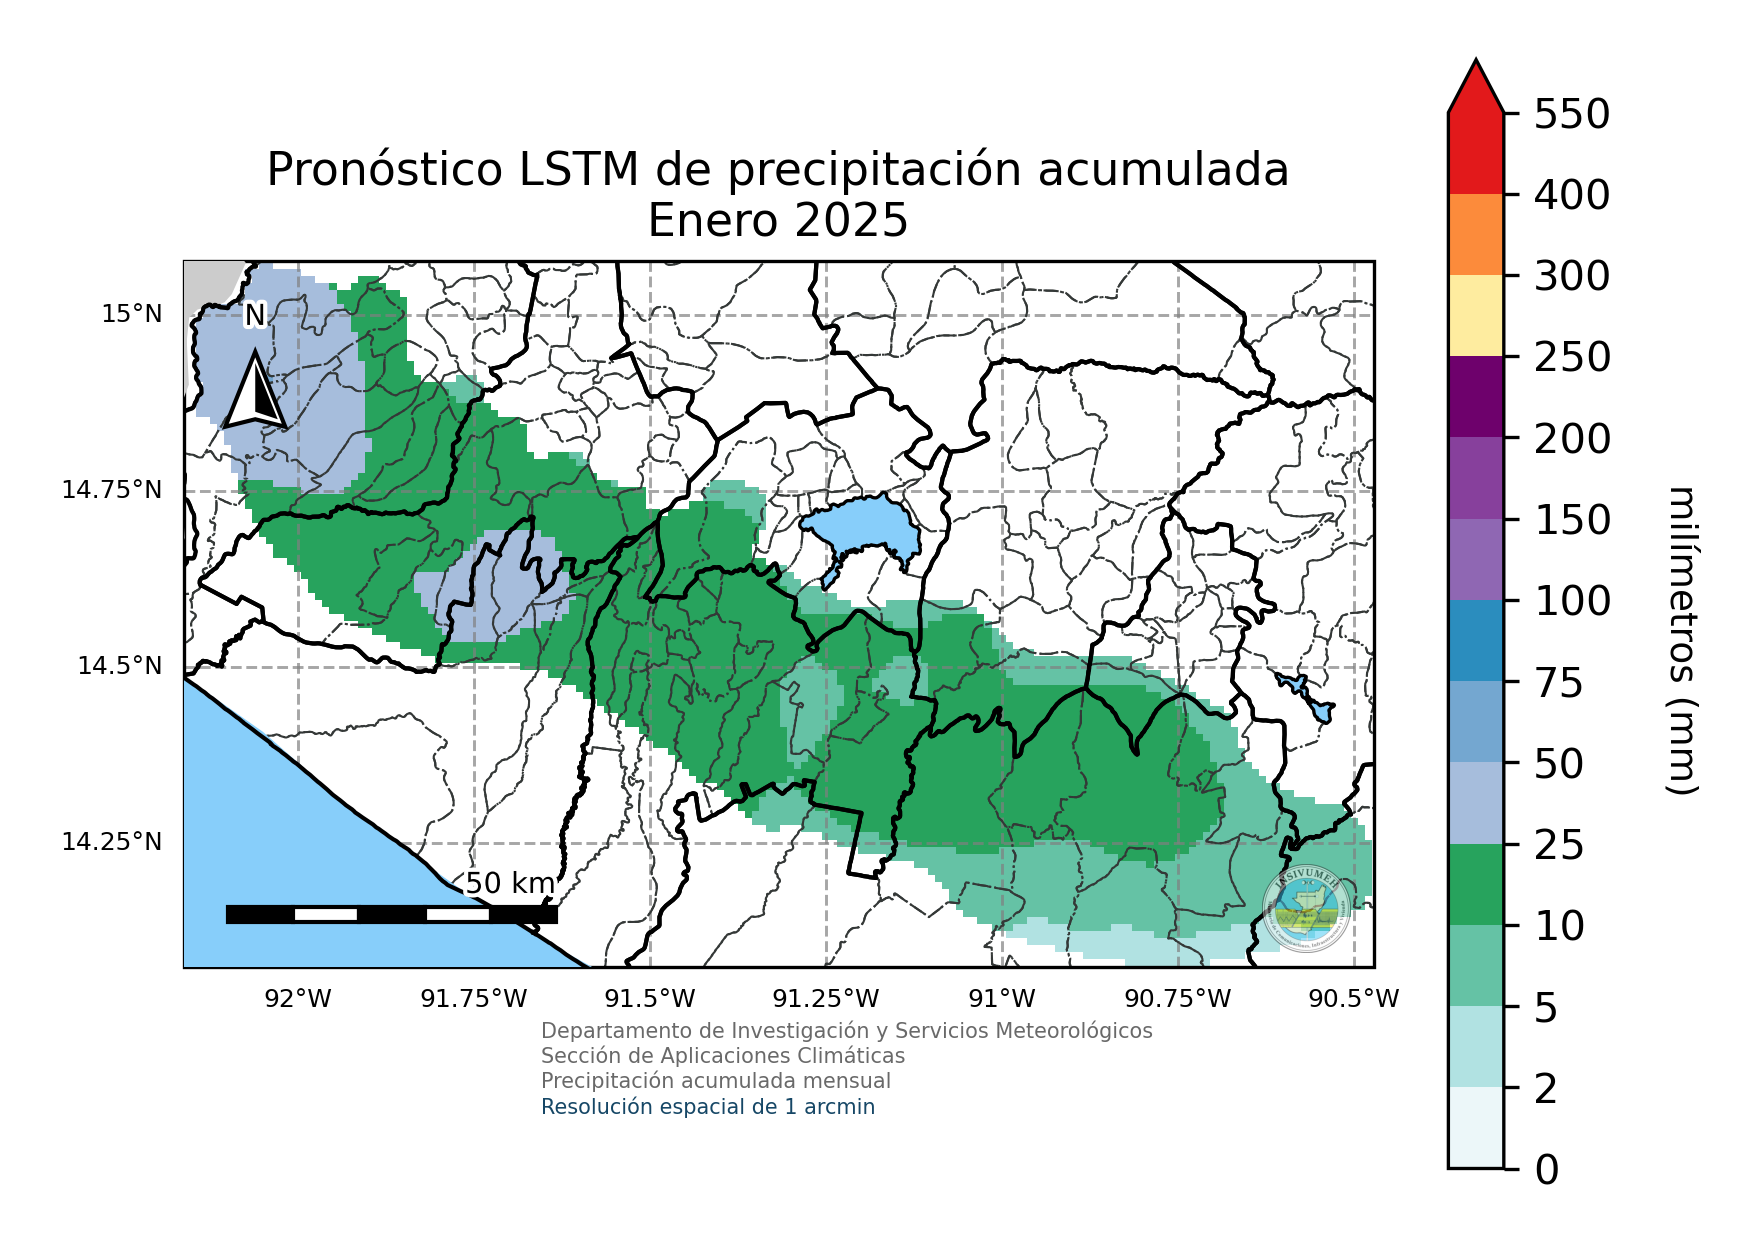
\includegraphics[width=\textwidth]{Informe/resultados/pronósticosLSTM/Pronóstico_LSTM_1_2025_Boca Costa_03.png}
	\end{subfigure}
	\hfill
	\begin{subfigure}[b]{0.45\textwidth}
		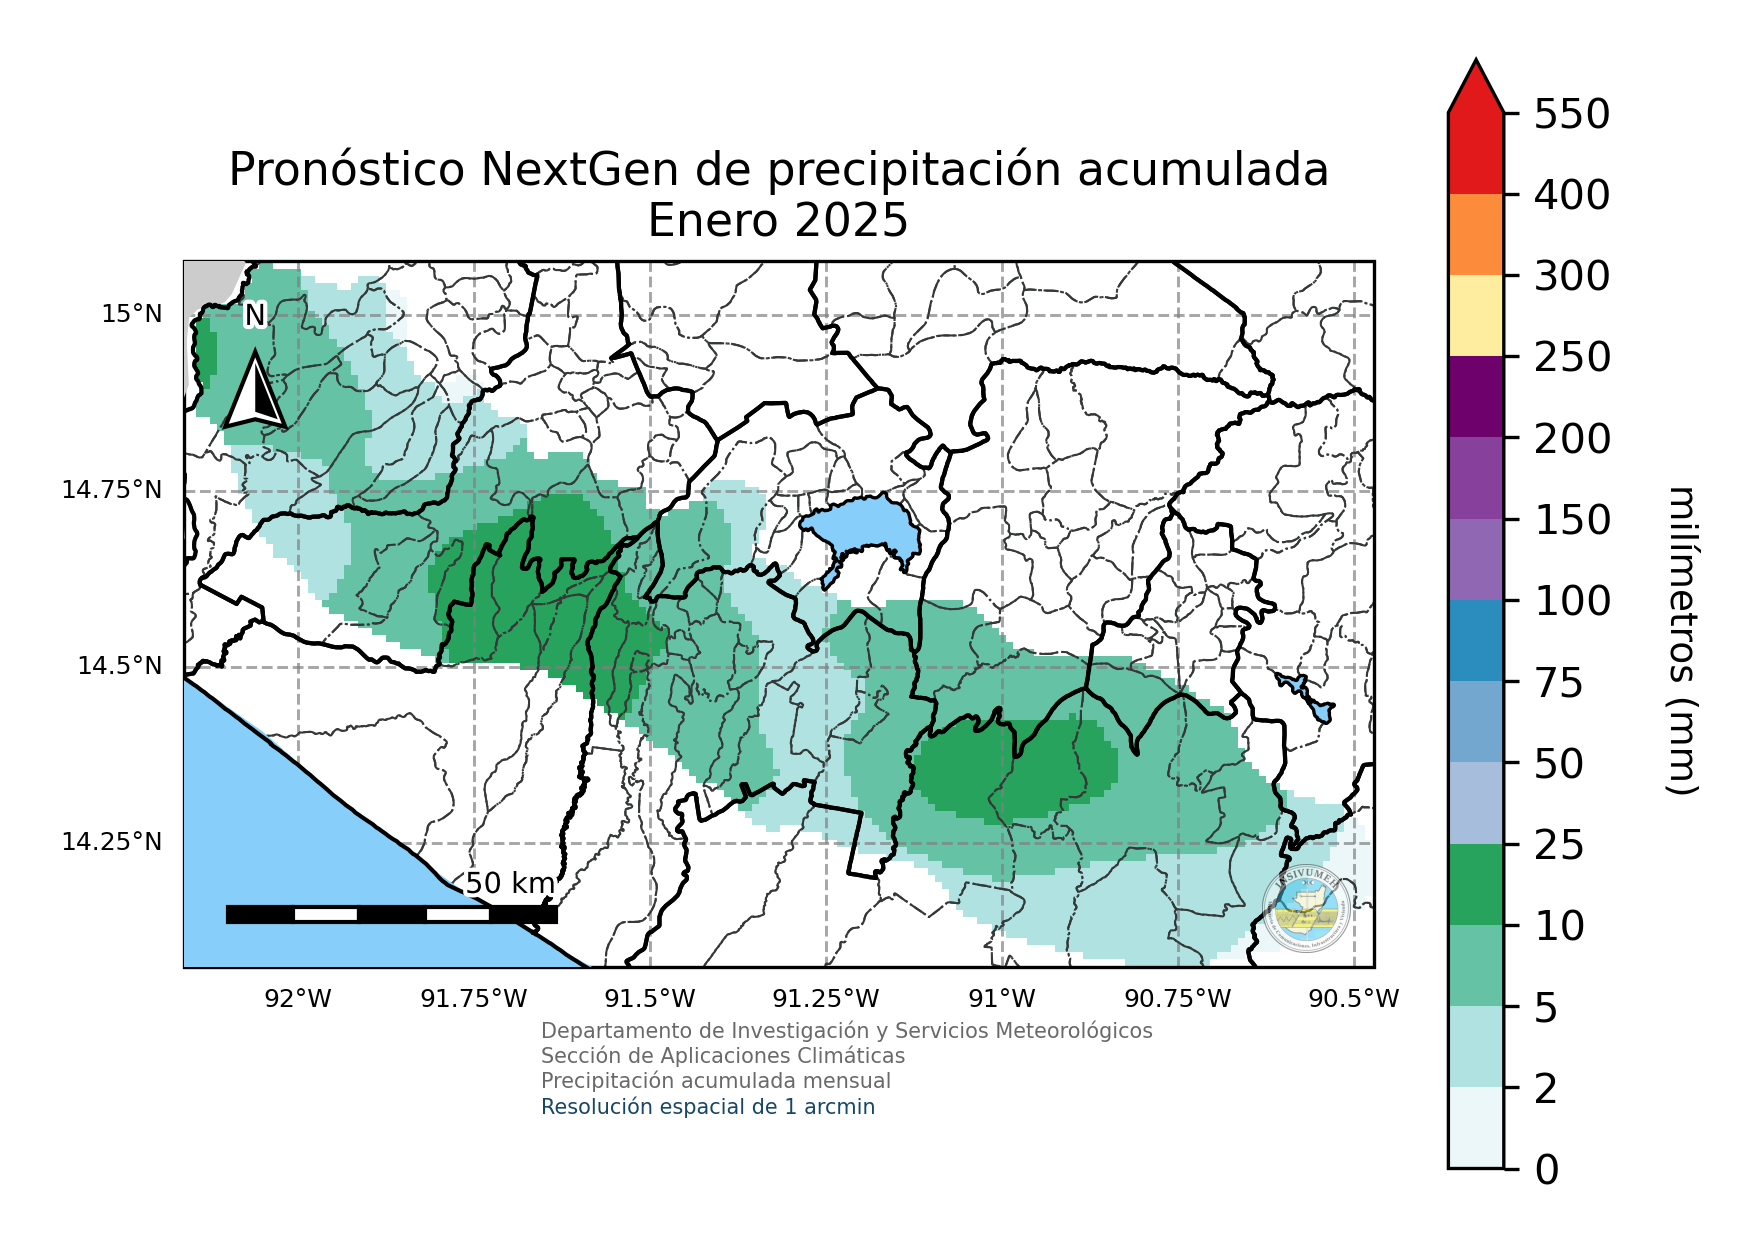
\includegraphics[width=\textwidth]{Informe/resultados/pronósticosNextGen/Pronóstico_NextGen_1_2025_Boca Costa_03.png}
	\end{subfigure}
	
	\vspace{-0.5em}
	
	\begin{subfigure}[b]{0.55\textwidth}
		\centering
		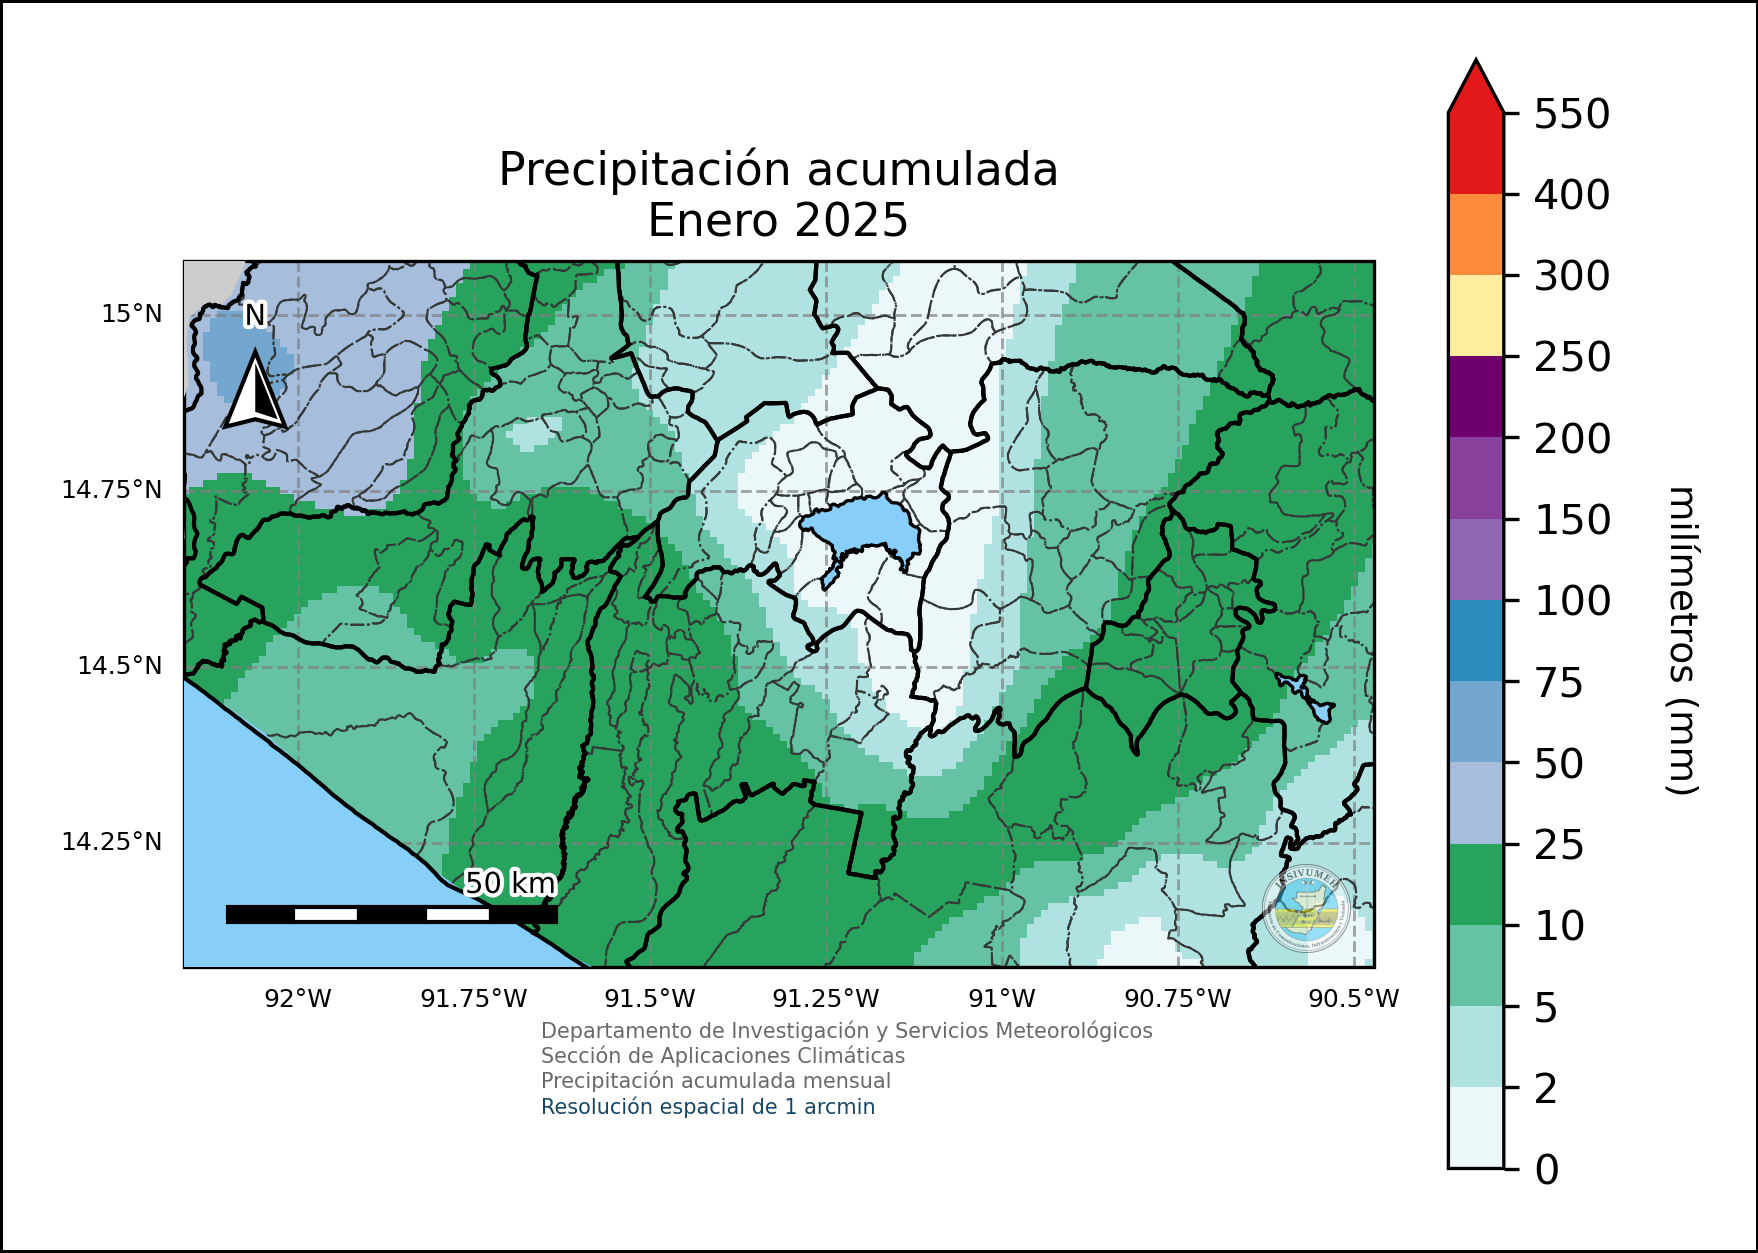
\includegraphics[width=\textwidth]{Informe/resultados/precipitación/Precipitación_1_2025_Boca Costa_03.png}
	\end{subfigure}
	
	\vspace{0.7em}
	
	% ==================================================
	% FEBRERO
	% ==================================================
	
	\textbf{Febrero 2025}
	
	\vspace{0.2em}
	
	\begin{subfigure}[b]{0.45\textwidth}
		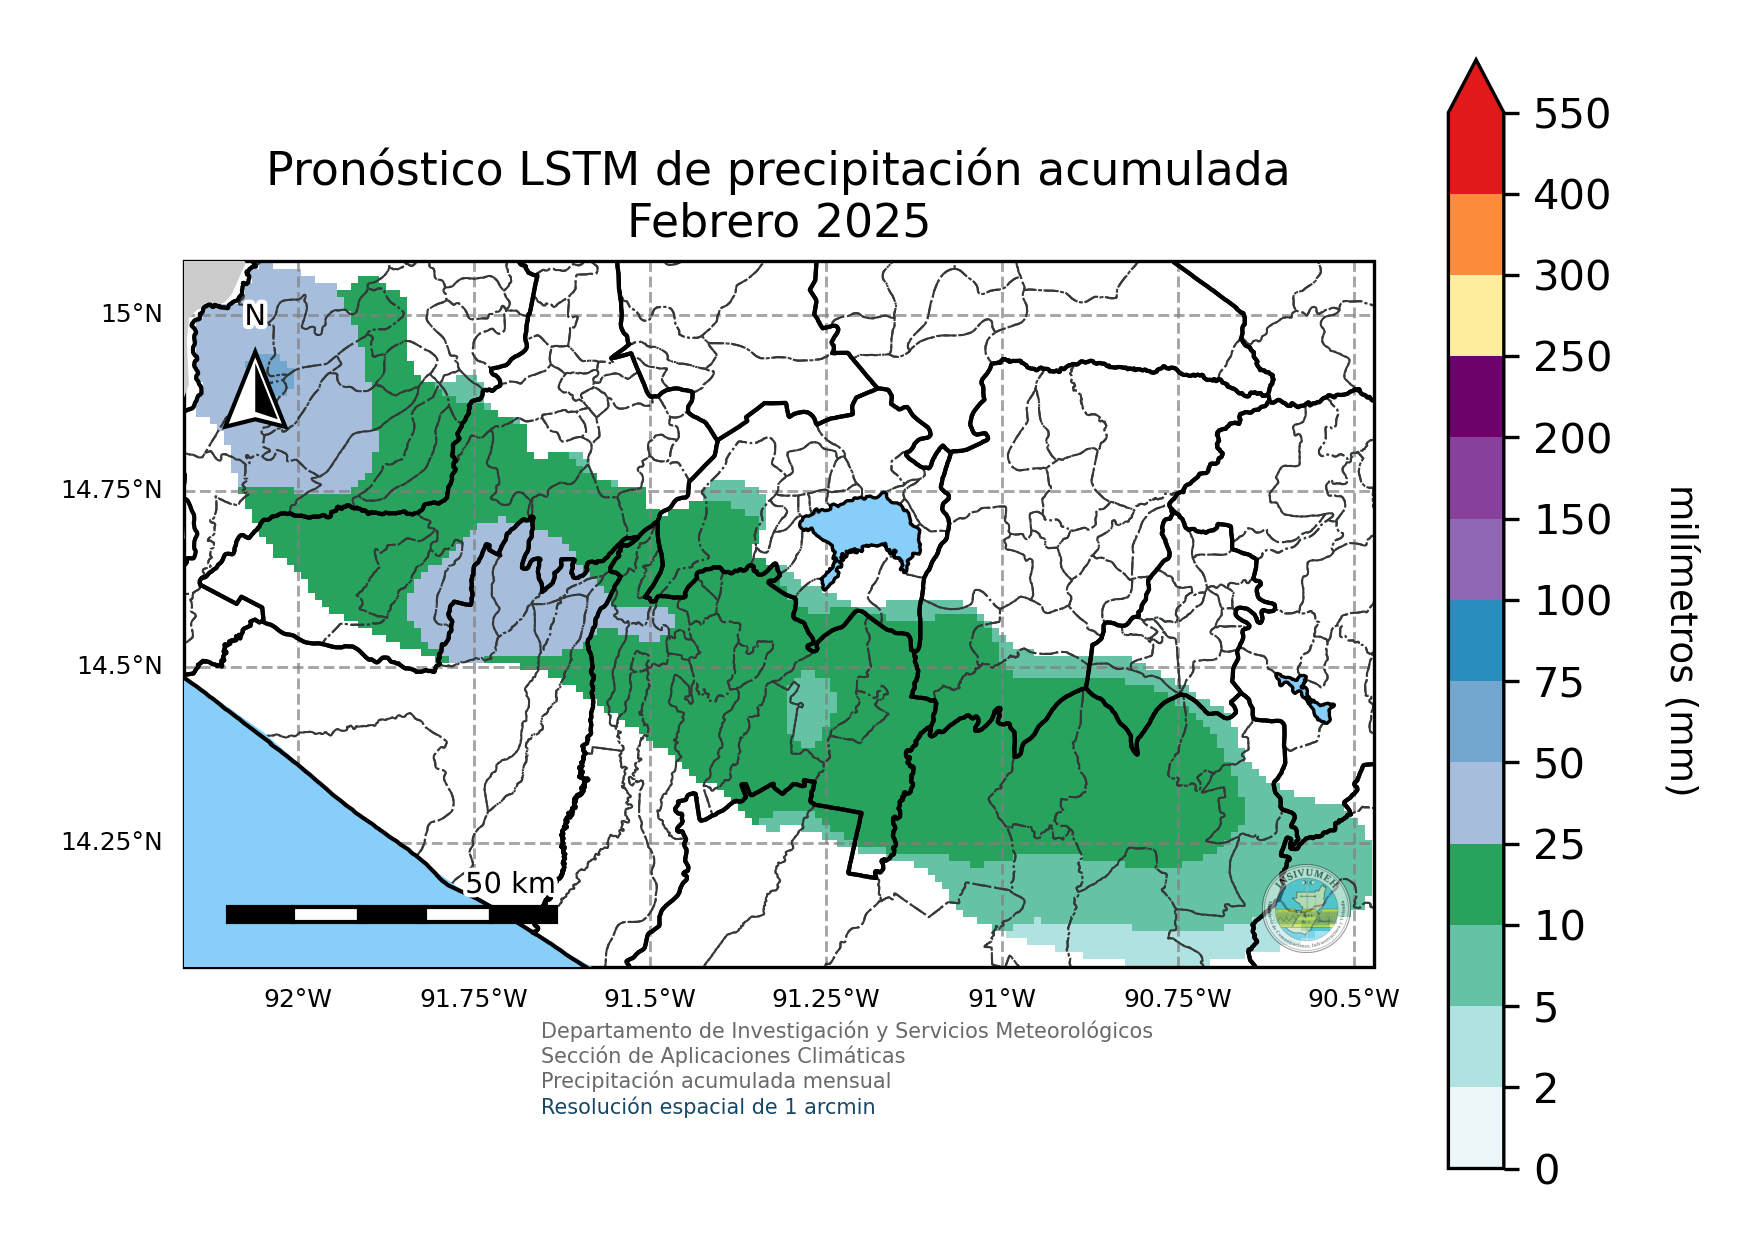
\includegraphics[width=\textwidth]{Informe/resultados/pronósticosLSTM/Pronóstico_LSTM_2_2025_Boca Costa_03.png}
	\end{subfigure}
	\hfill
	\begin{subfigure}[b]{0.45\textwidth}
		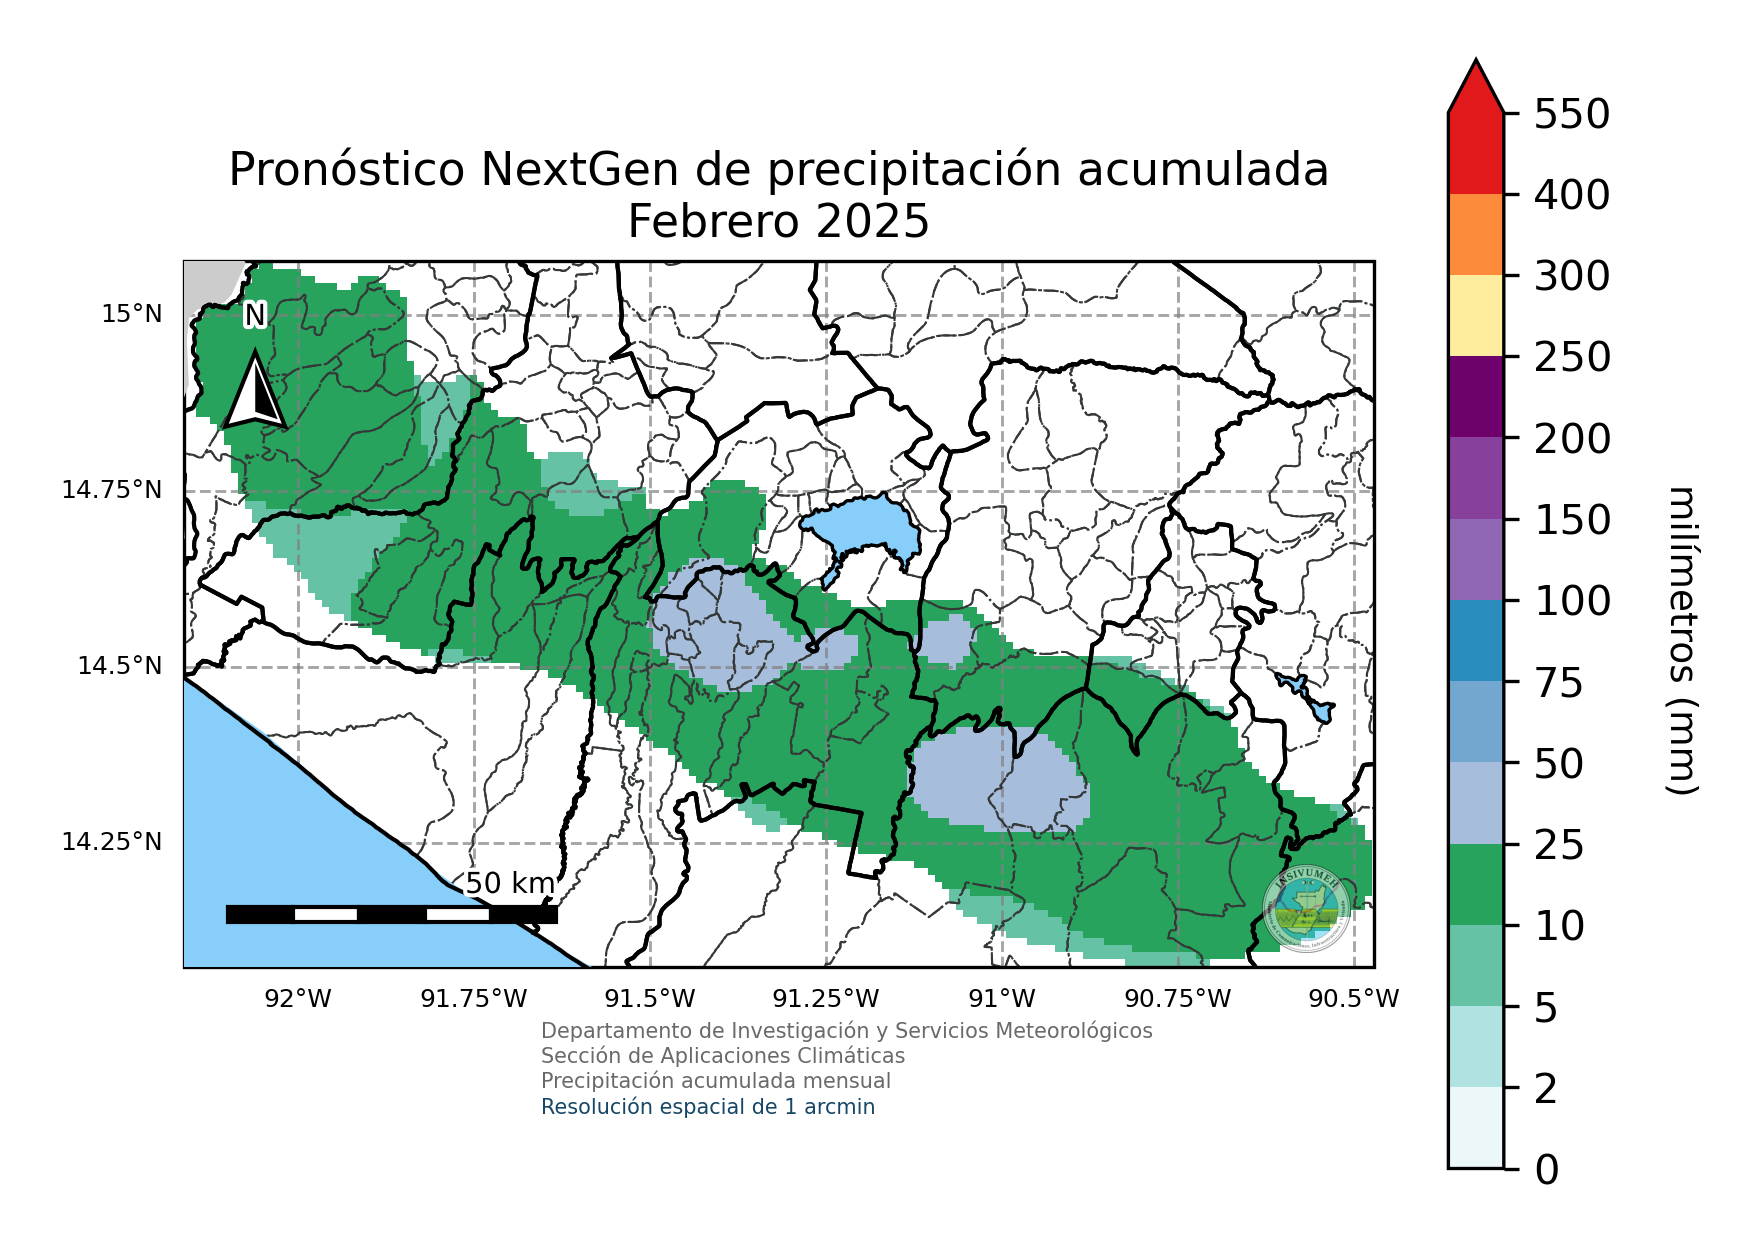
\includegraphics[width=\textwidth]{Informe/resultados/pronósticosNextGen/Pronóstico_NextGen_2_2025_Boca Costa_03.png}
	\end{subfigure}
	
	\vspace{-0.5em}
	
	\begin{subfigure}[b]{0.55\textwidth}
		\centering
		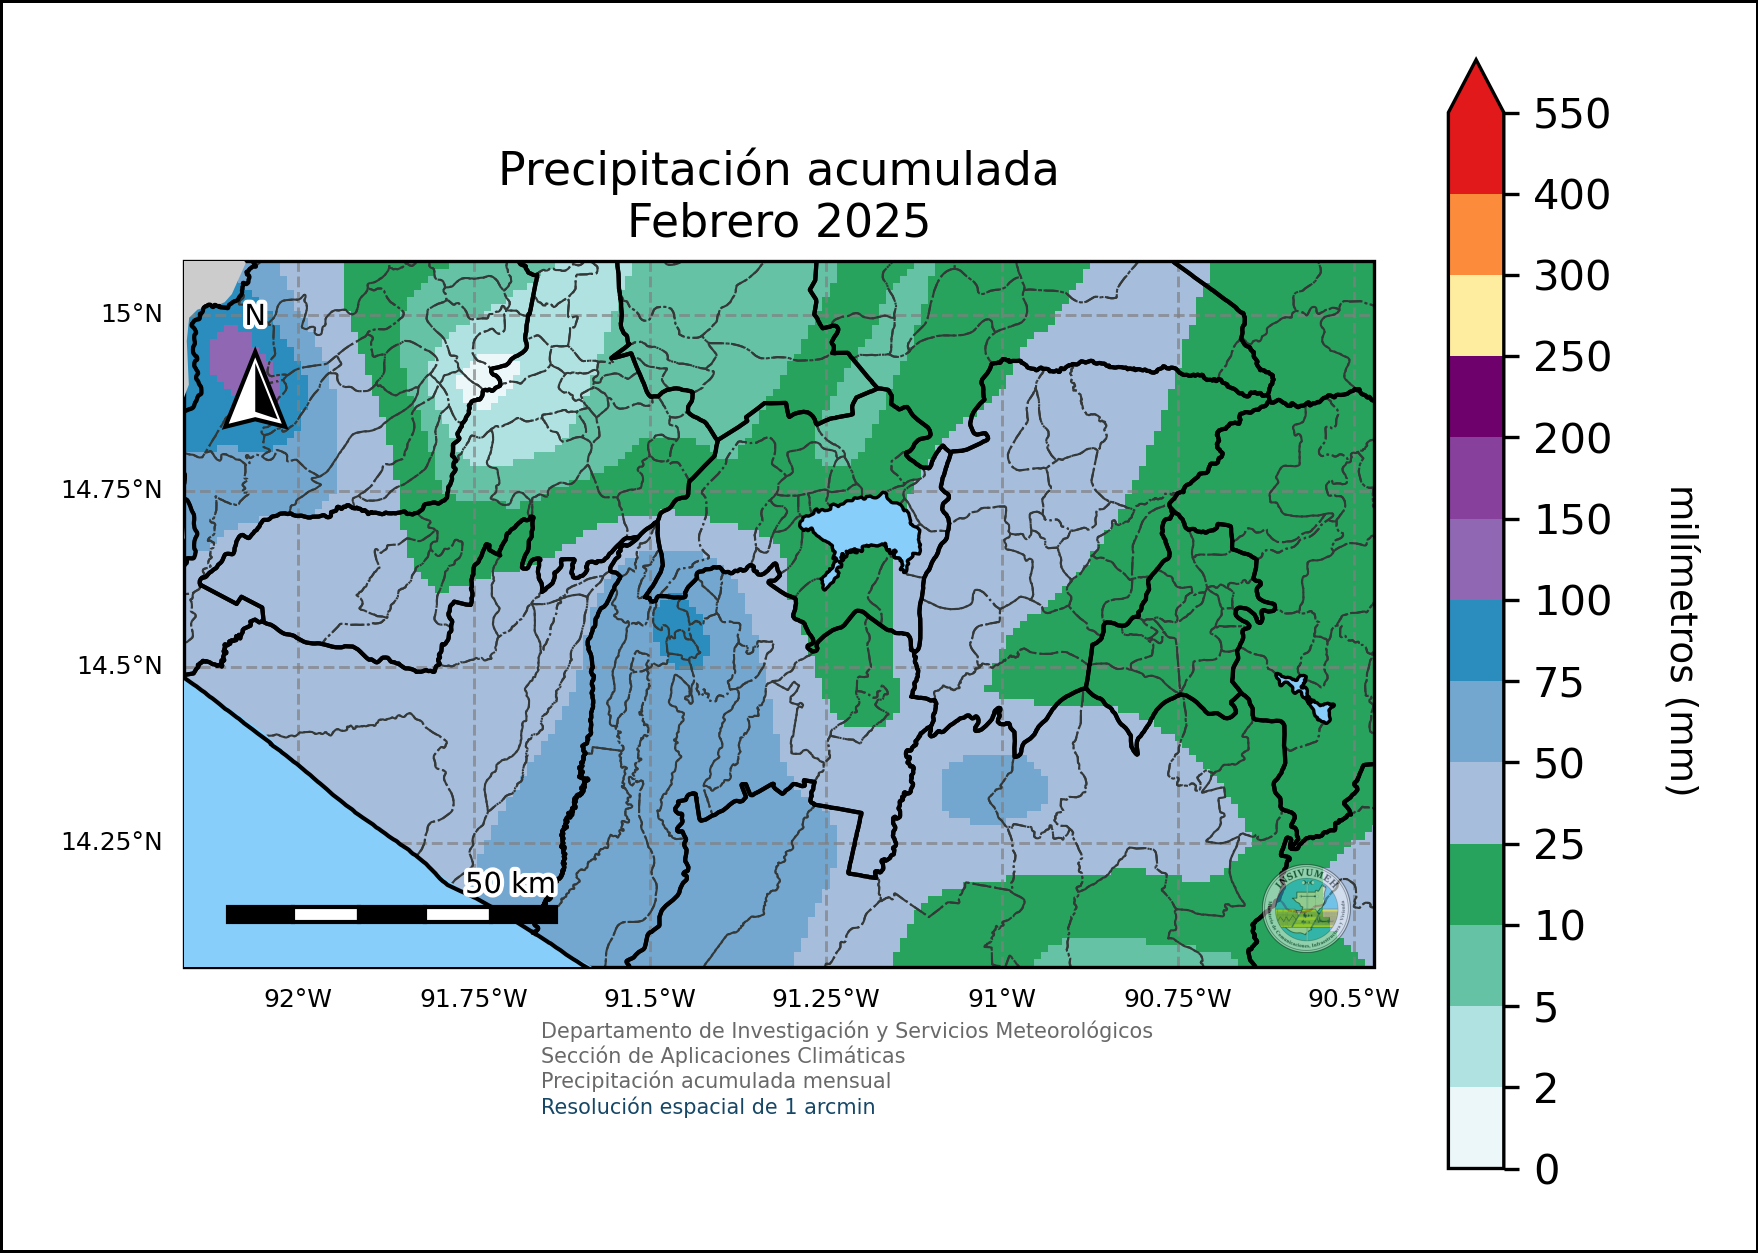
\includegraphics[width=\textwidth]{Informe/resultados/precipitación/Precipitación_2_2025_Boca Costa_03.png}
	\end{subfigure}
\end{figure}

\begin{figure}[!htbp]
	\centering
	% ==================================================
	% MARZO
	% ==================================================
	
	\textbf{Marzo 2025}
	
	\vspace{0.2em}
	
	\begin{subfigure}[b]{0.45\textwidth}
		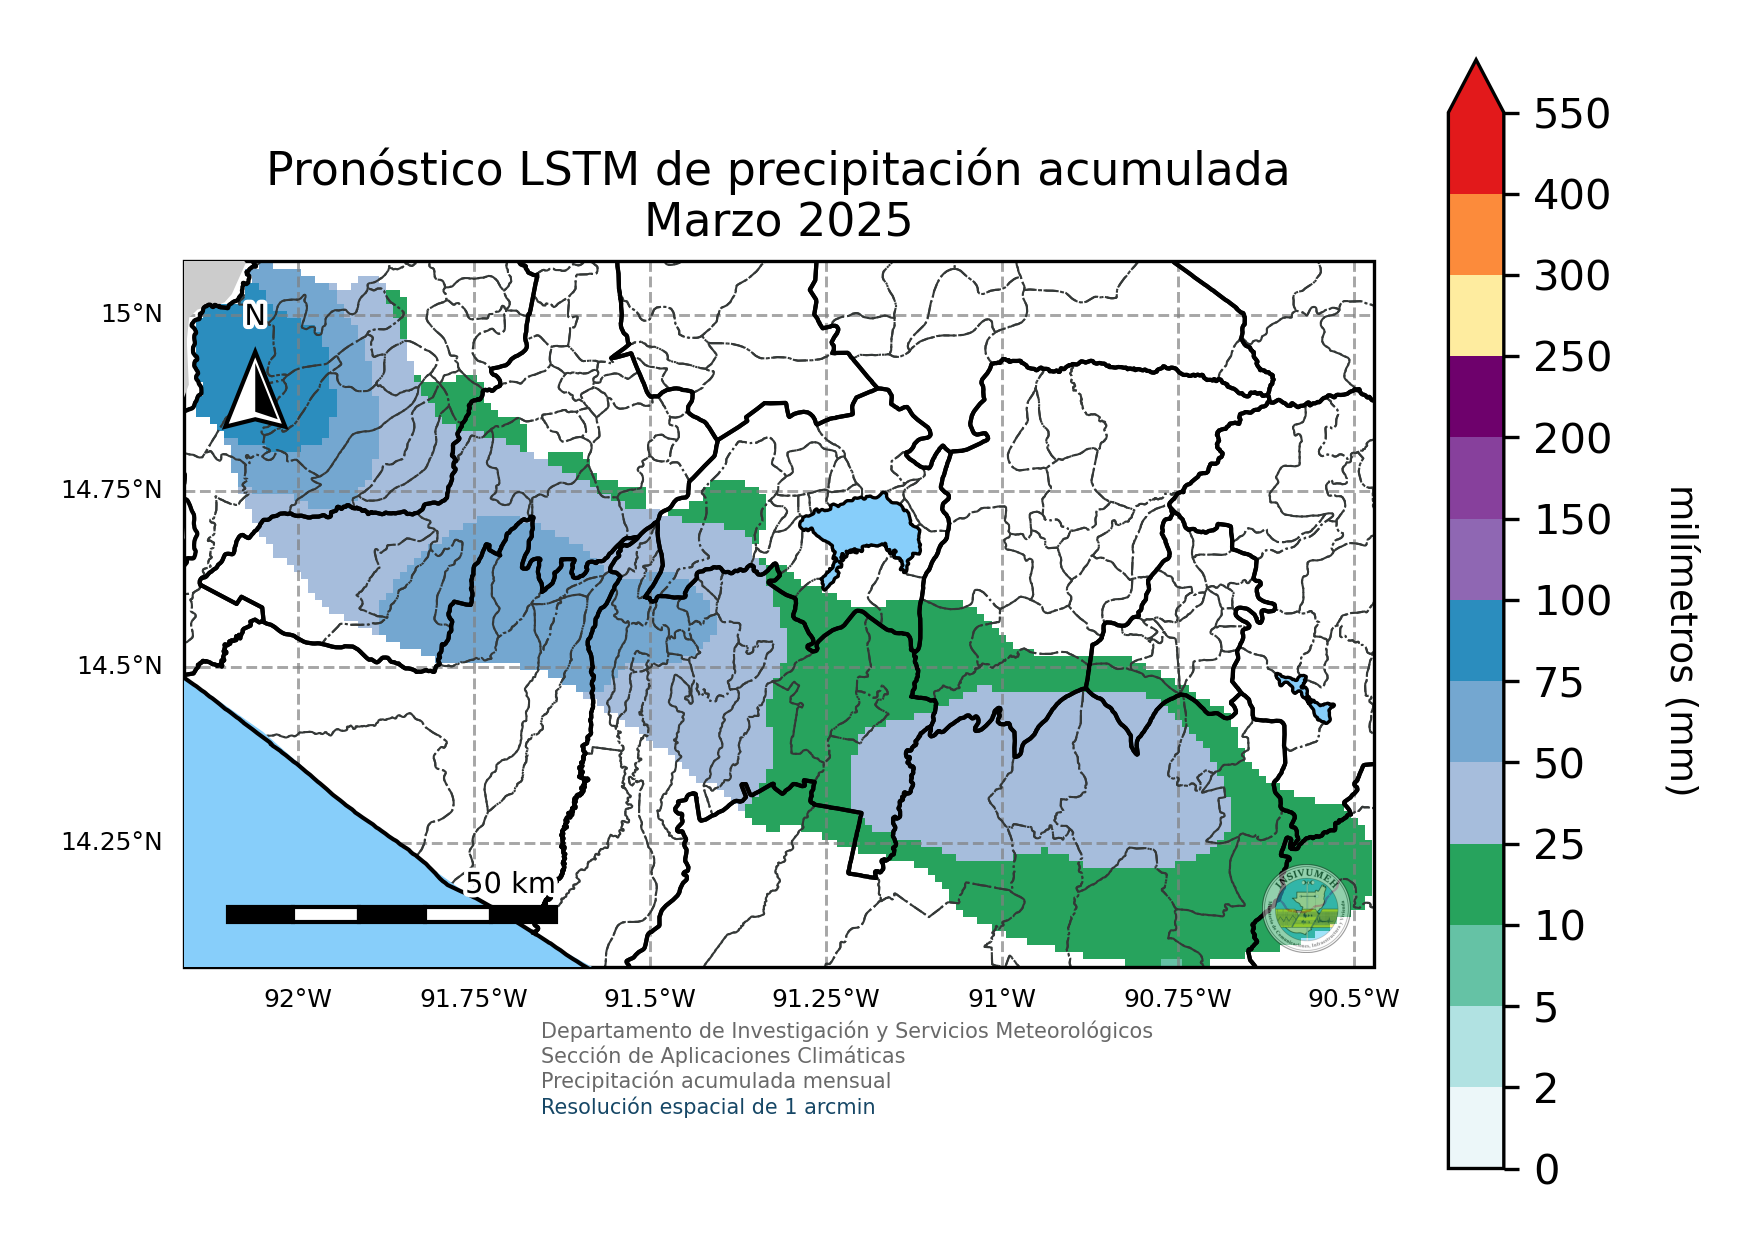
\includegraphics[width=\textwidth]{Informe/resultados/pronósticosLSTM/Pronóstico_LSTM_3_2025_Boca Costa_03.png}
	\end{subfigure}
	\hfill
	\begin{subfigure}[b]{0.45\textwidth}
		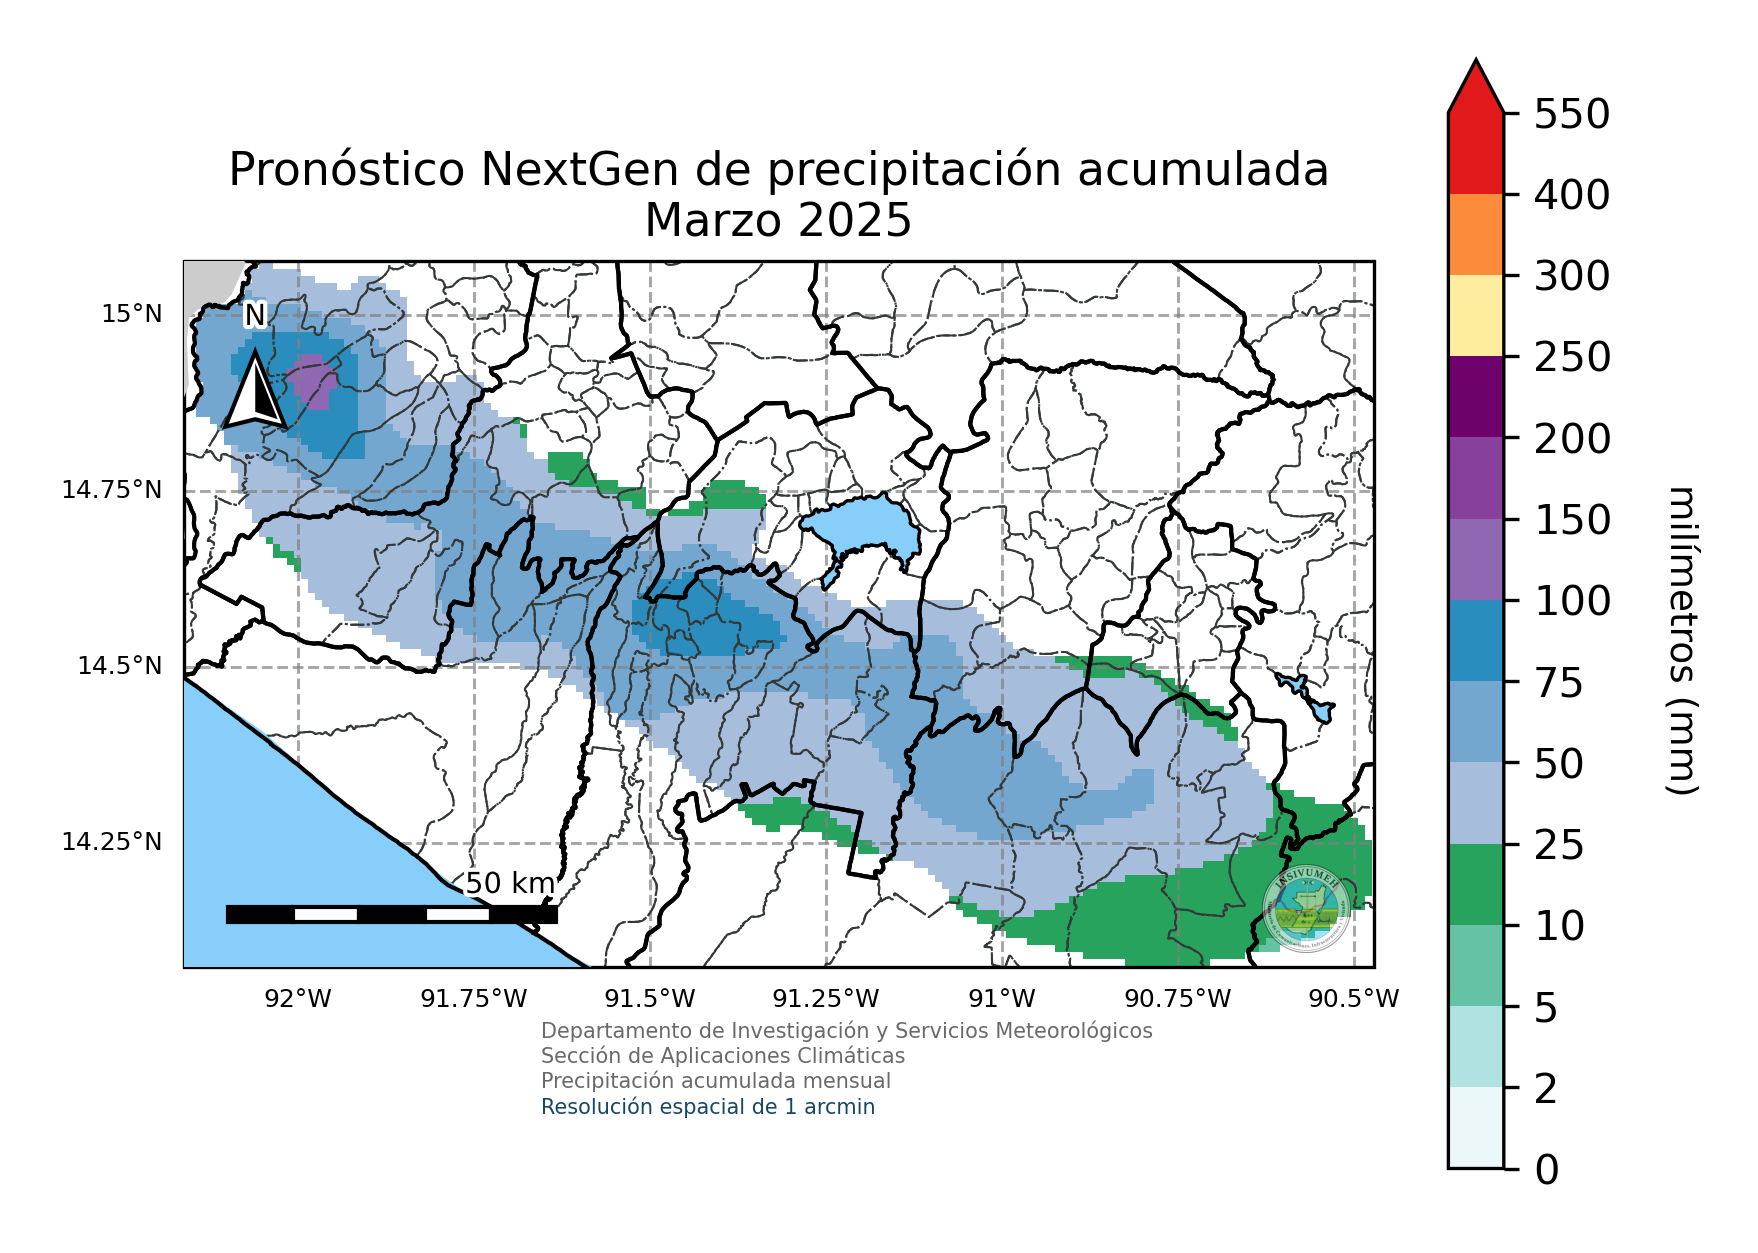
\includegraphics[width=\textwidth]{Informe/resultados/pronósticosNextGen/Pronóstico_NextGen_3_2025_Boca Costa_03.png}
	\end{subfigure}
	
	\vspace{-0.5em}
	
	\begin{subfigure}[b]{0.55\textwidth}
		\centering
		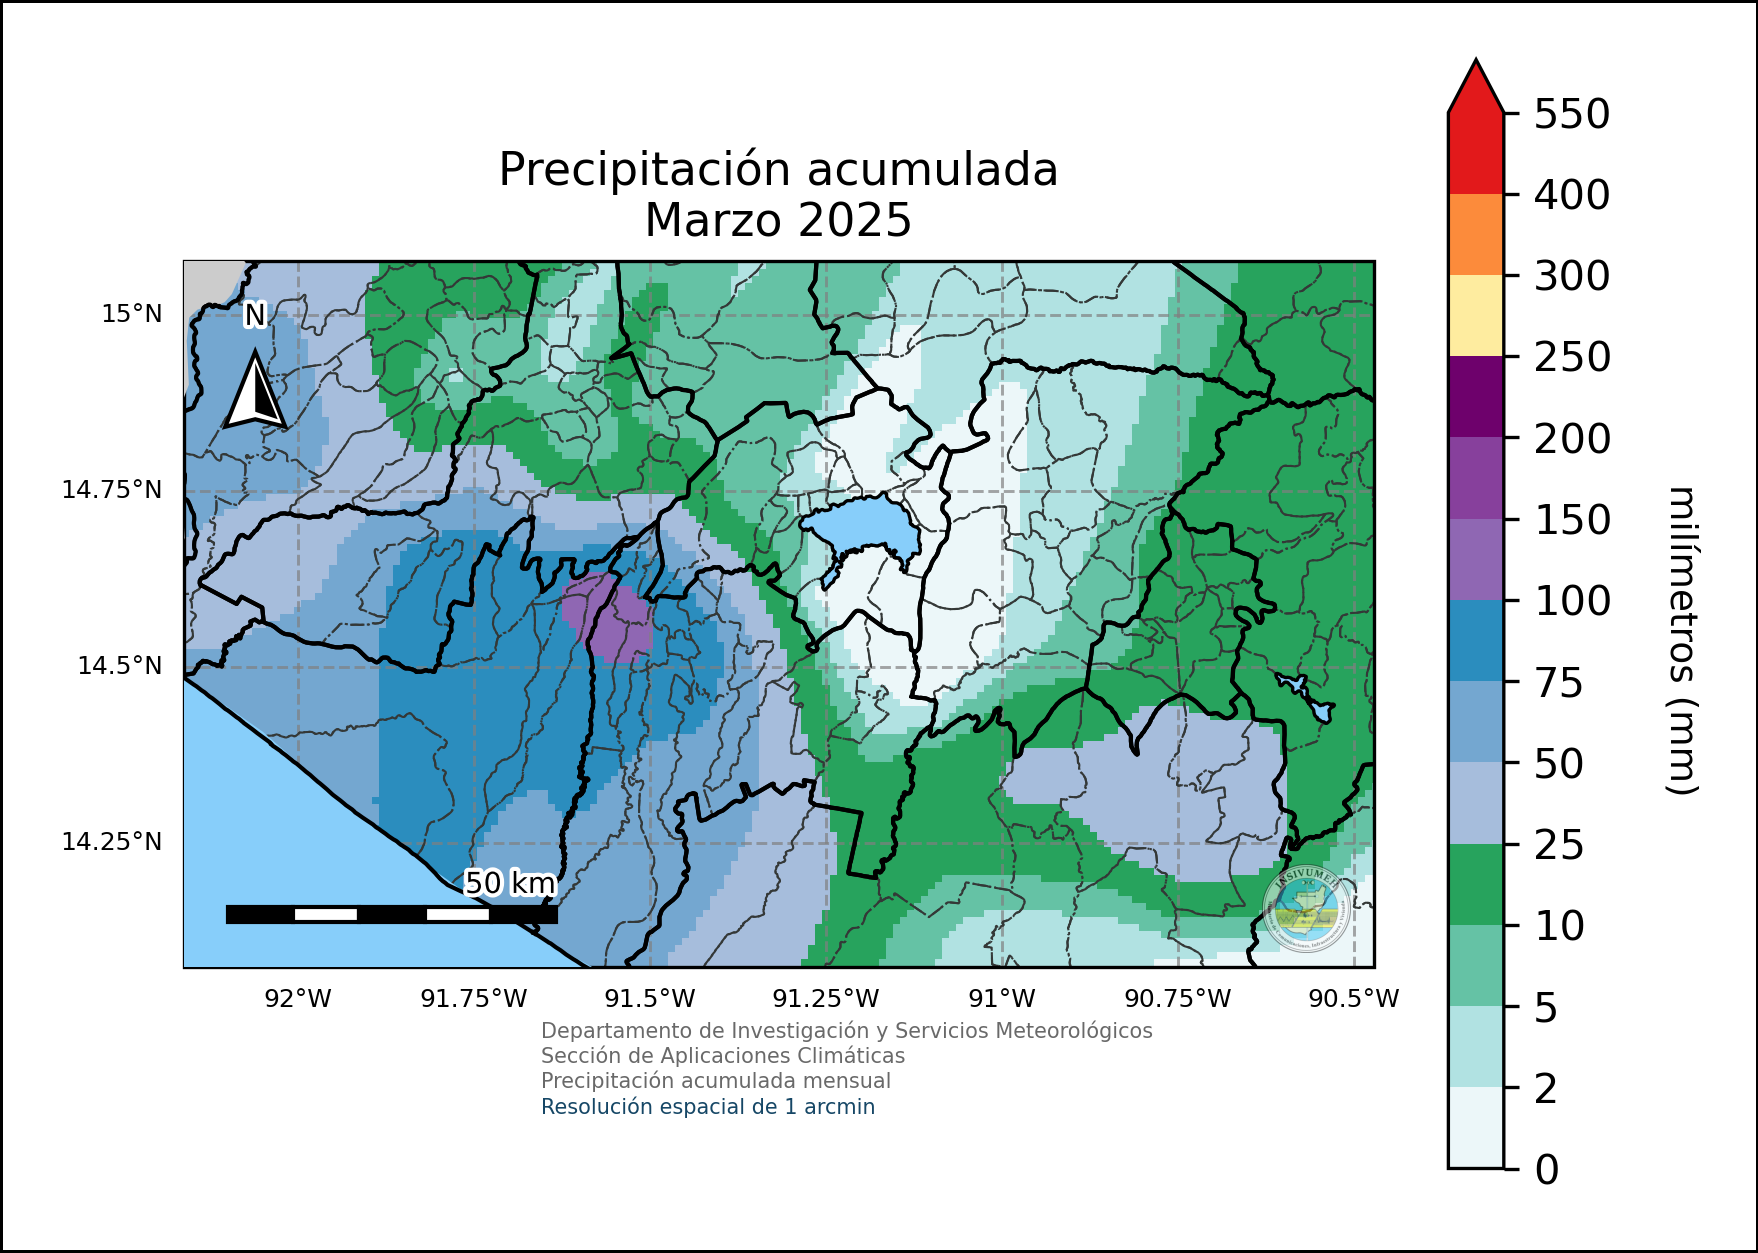
\includegraphics[width=\textwidth]{Informe/resultados/precipitación/Precipitación_3_2025_Boca Costa_03.png}
	\end{subfigure}
	
	\vspace{0.7em}
	
	% ==================================================
	% ABRIL
	% ==================================================
	
	\textbf{Abril 2025}
	
	\vspace{0.2em}
	
	\begin{subfigure}[b]{0.45\textwidth}
		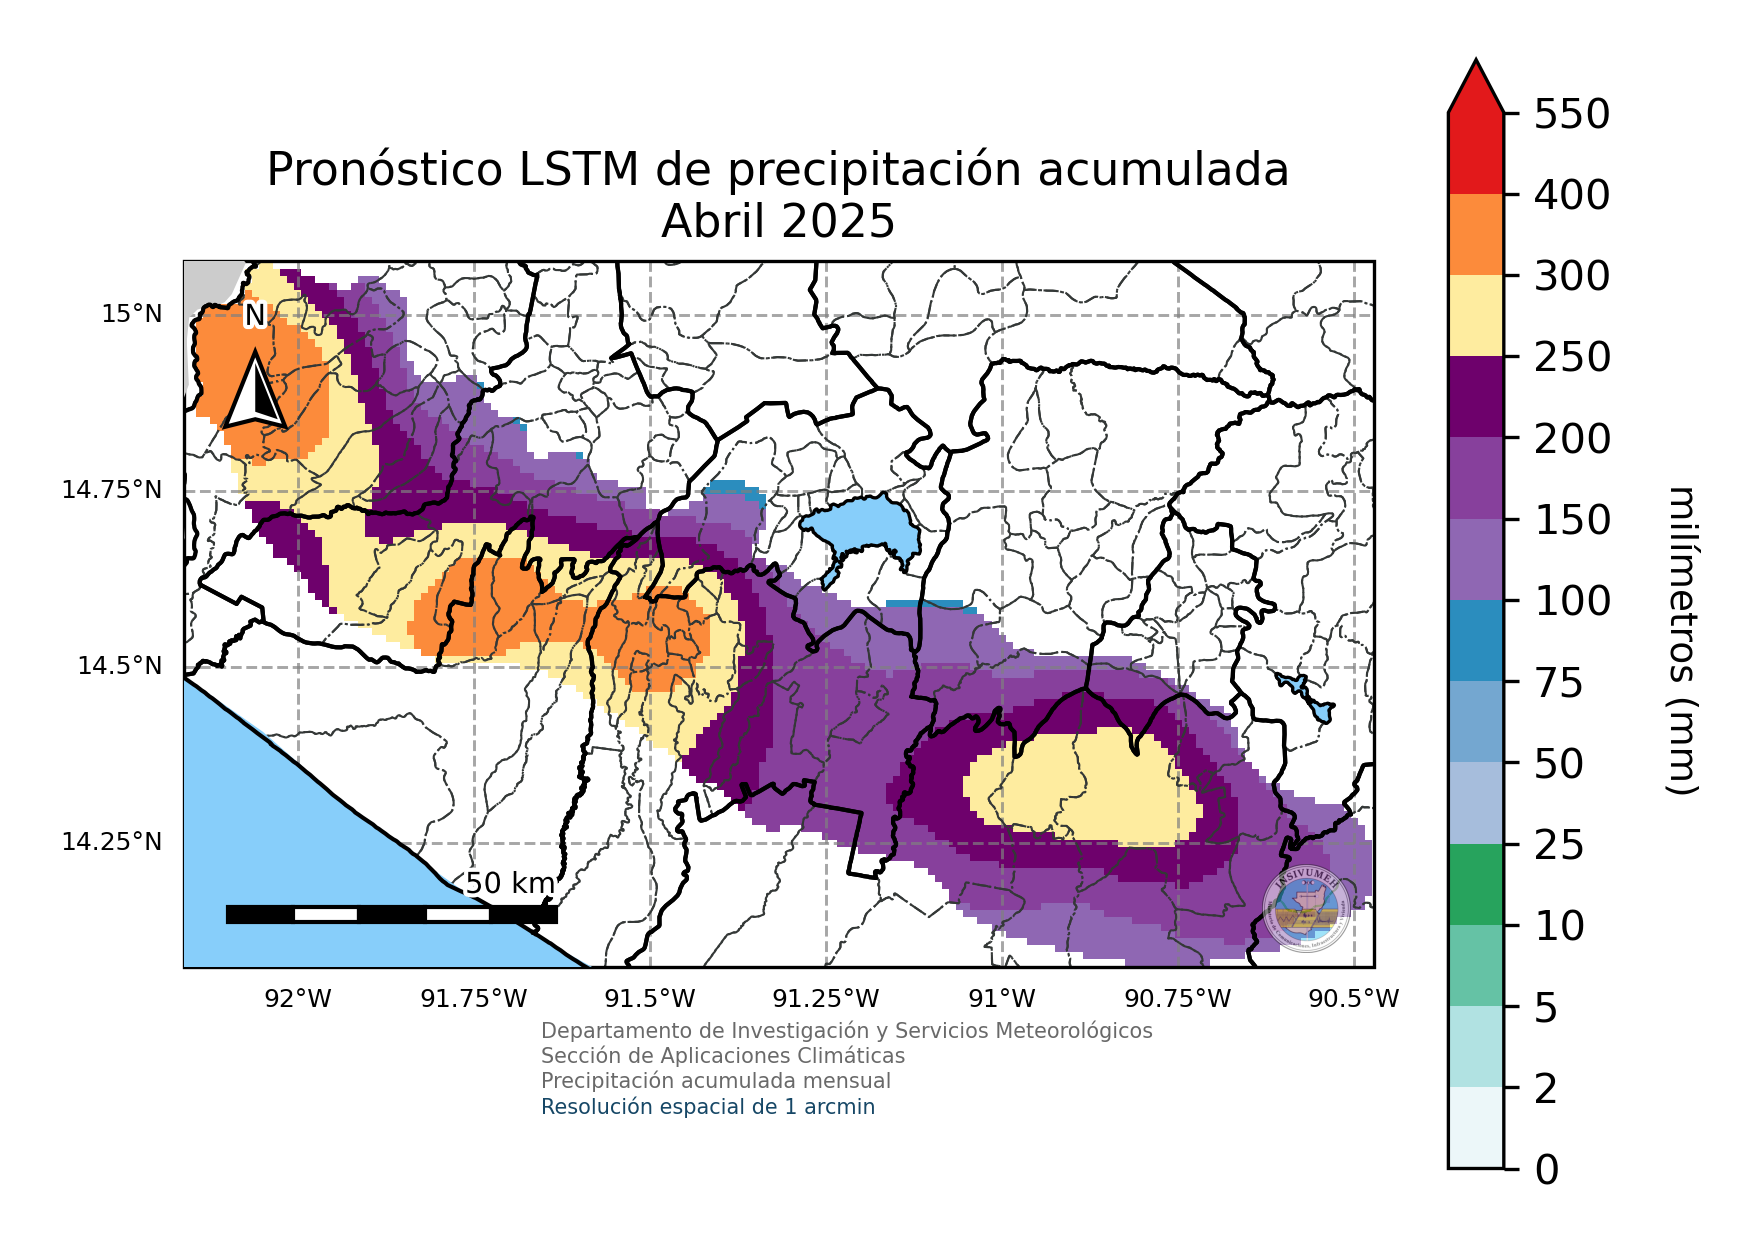
\includegraphics[width=\textwidth]{Informe/resultados/pronósticosLSTM/Pronóstico_LSTM_4_2025_Boca Costa_03.png}
	\end{subfigure}
	\hfill
	\begin{subfigure}[b]{0.45\textwidth}
		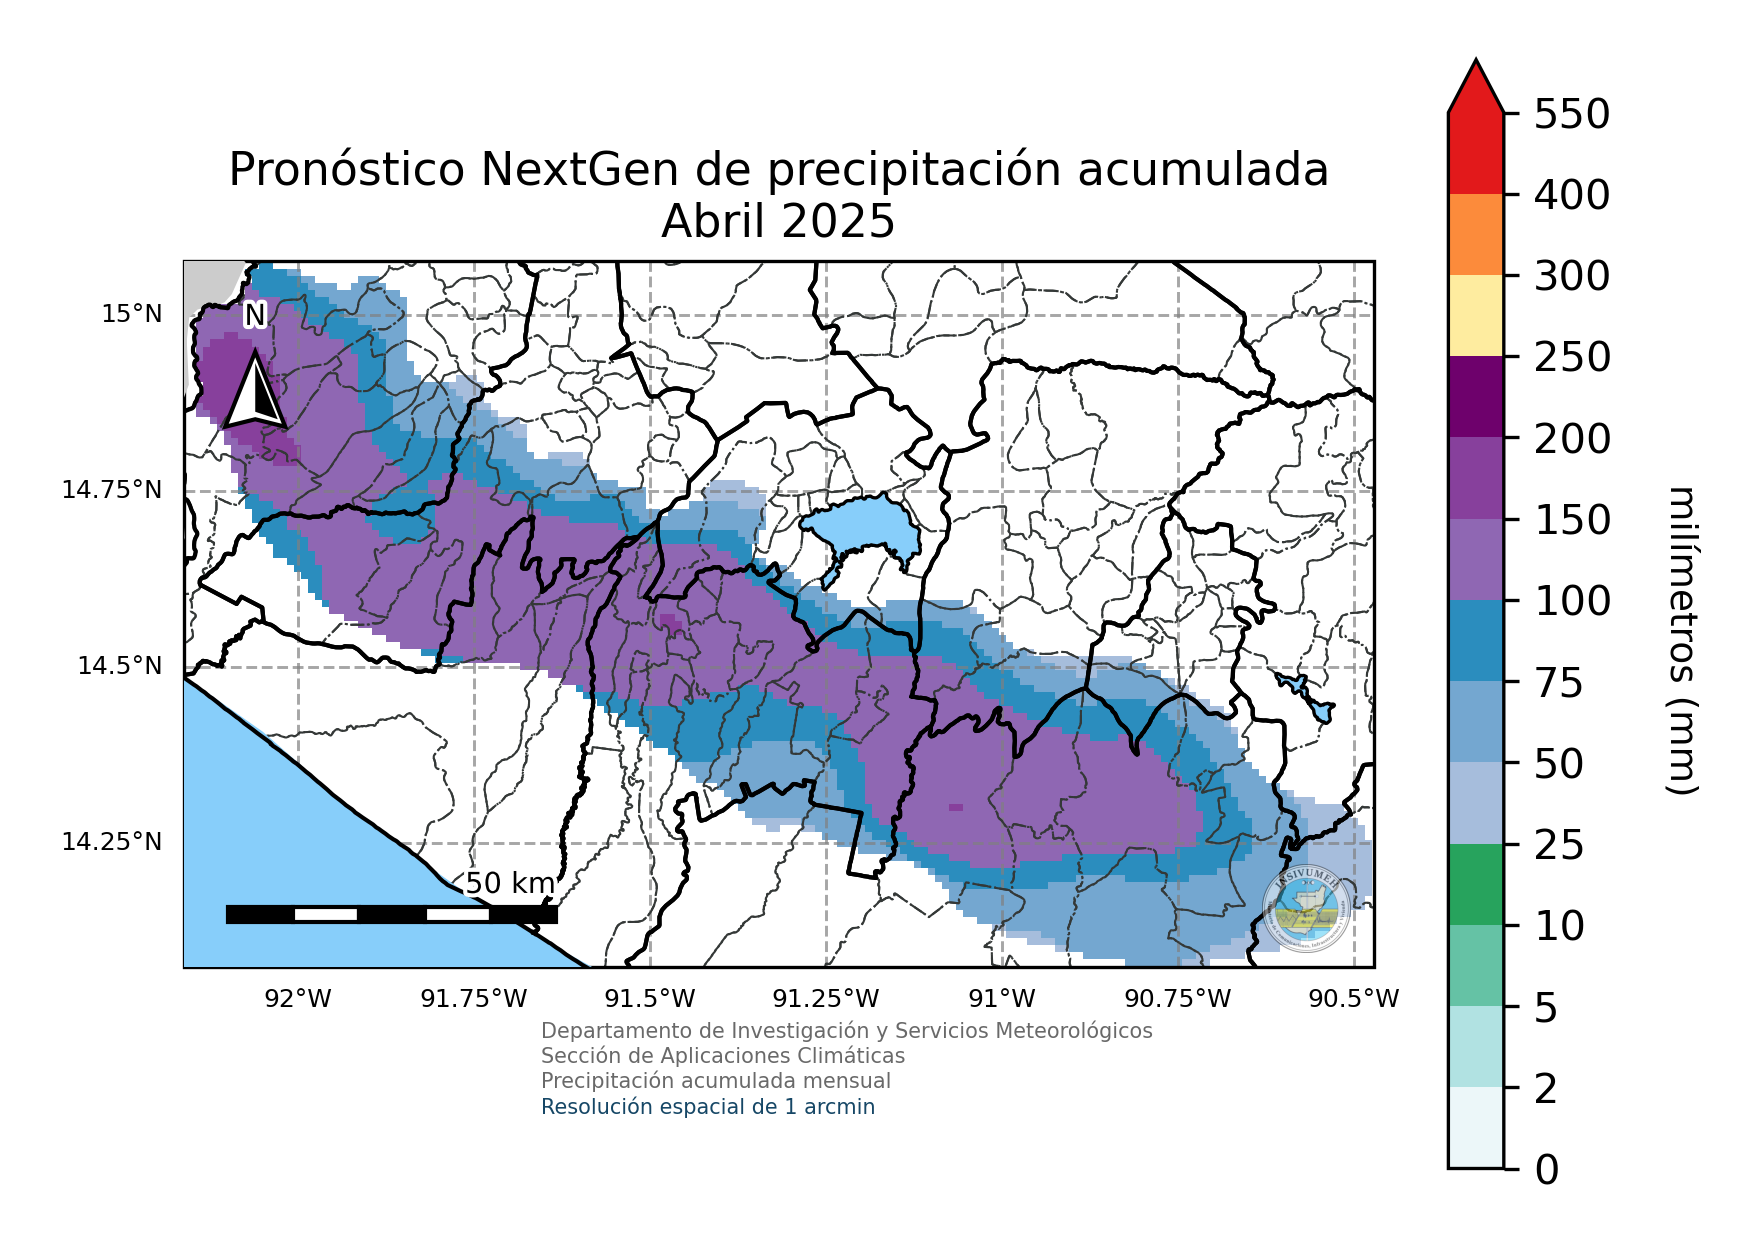
\includegraphics[width=\textwidth]{Informe/resultados/pronósticosNextGen/Pronóstico_NextGen_4_2025_Boca Costa_03.png}
	\end{subfigure}
	
	\vspace{-0.5em}
	
	\begin{subfigure}[b]{0.55\textwidth}
		\centering
		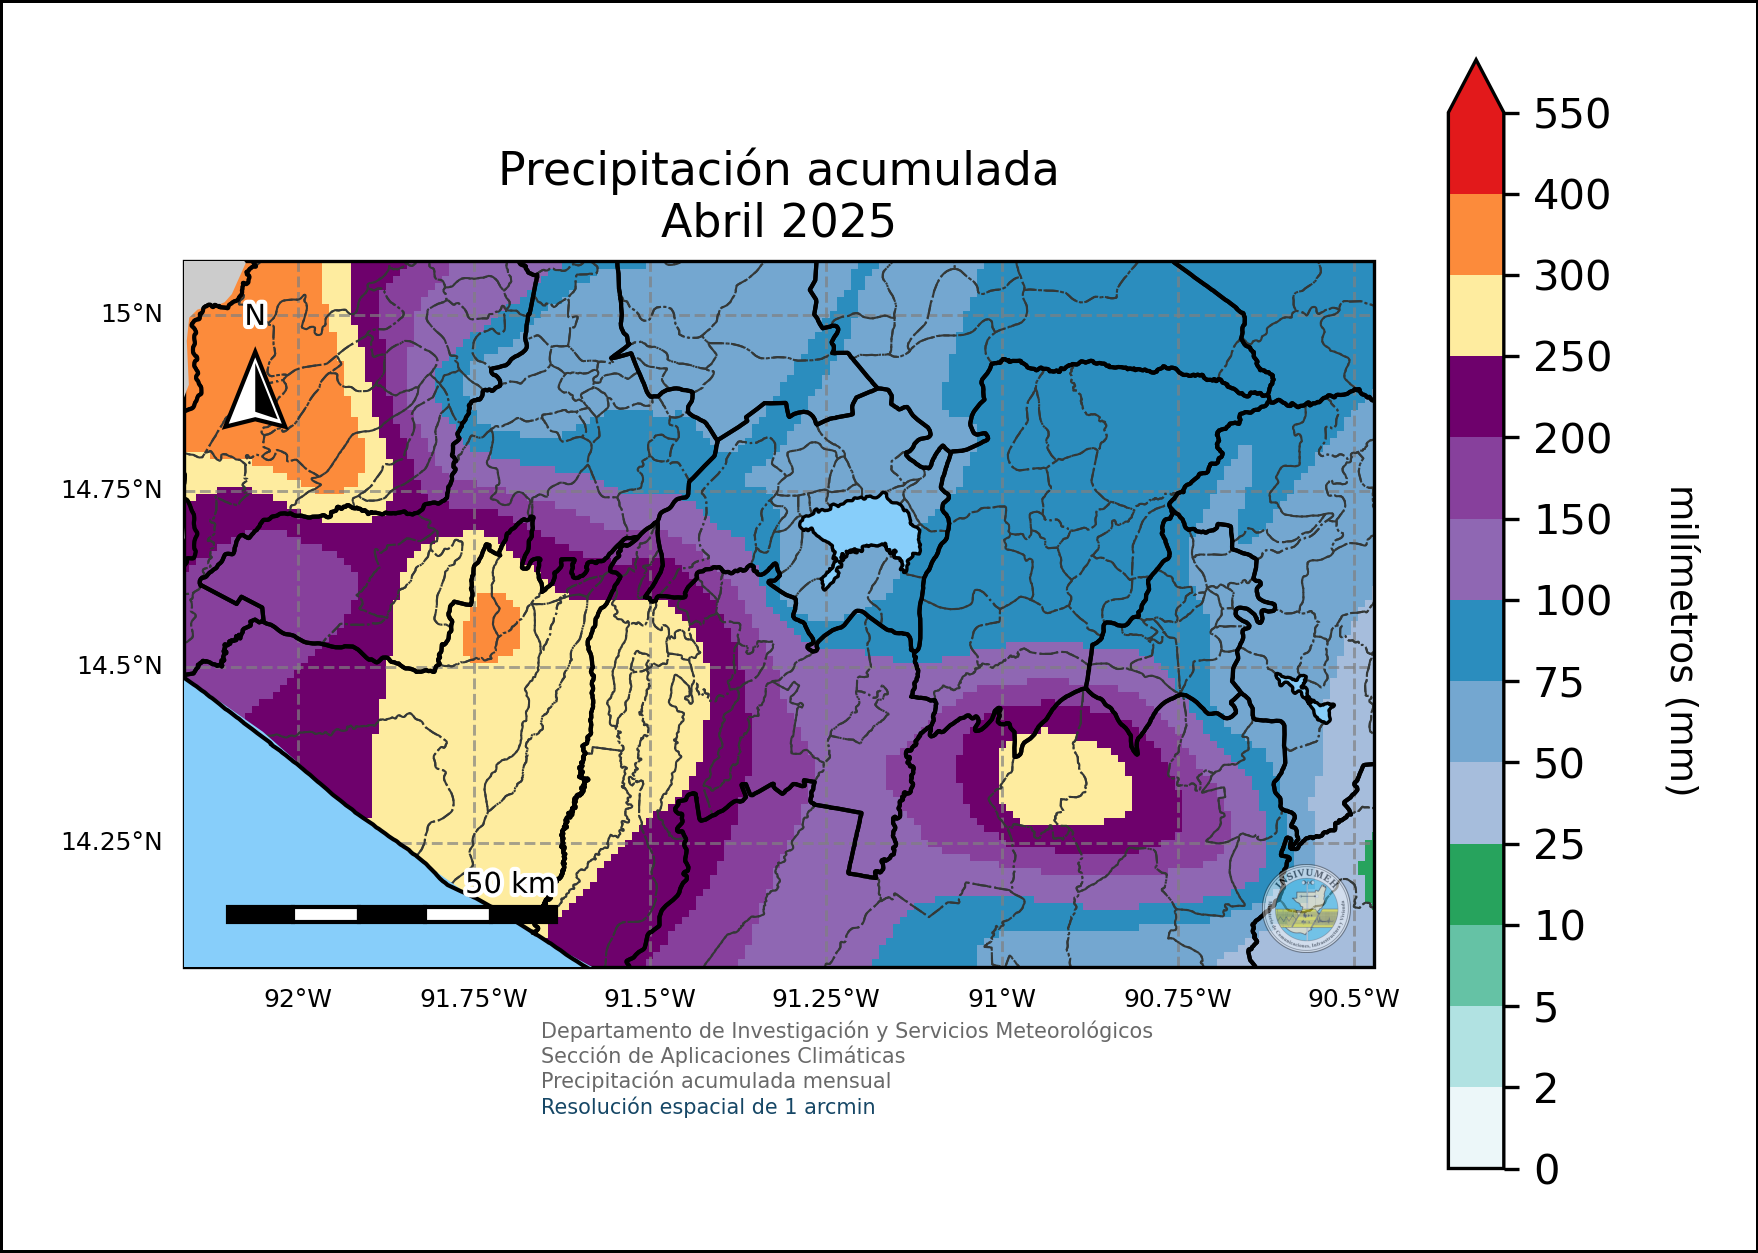
\includegraphics[width=\textwidth]{Informe/resultados/precipitación/Precipitación_4_2025_Boca Costa_03.png}
	\end{subfigure}
	```
	
\end{figure}

\begin{figure}[!htbp]
	\centering
	% ==================================================
	% MAYO
	% ==================================================
	
	\textbf{Mayo 2025}
	
	\vspace{0.2em}
	
	\begin{subfigure}[b]{0.45\textwidth}
		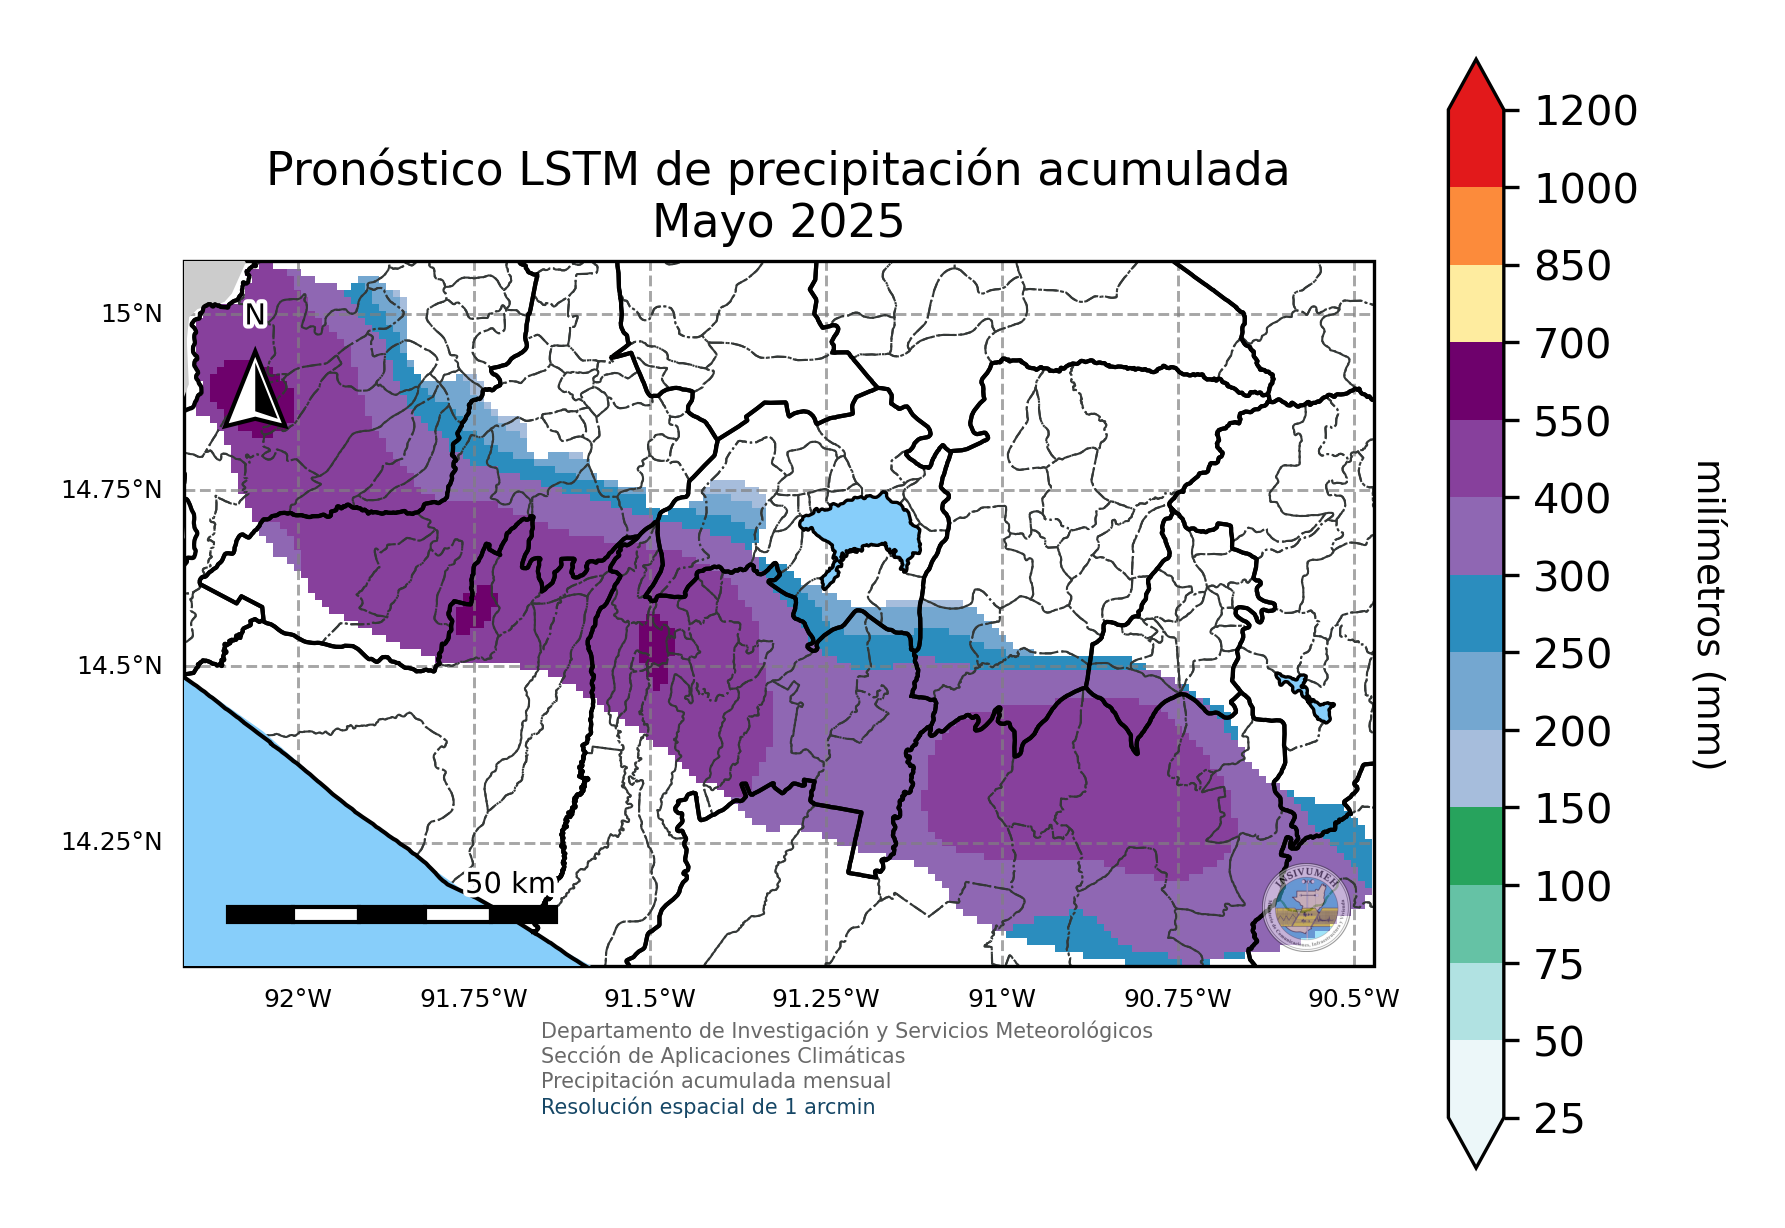
\includegraphics[width=\textwidth]{Informe/resultados/pronósticosLSTM/Pronóstico_LSTM_5_2025_Boca Costa_03.png}
	\end{subfigure}
	\hfill
	\begin{subfigure}[b]{0.45\textwidth}
		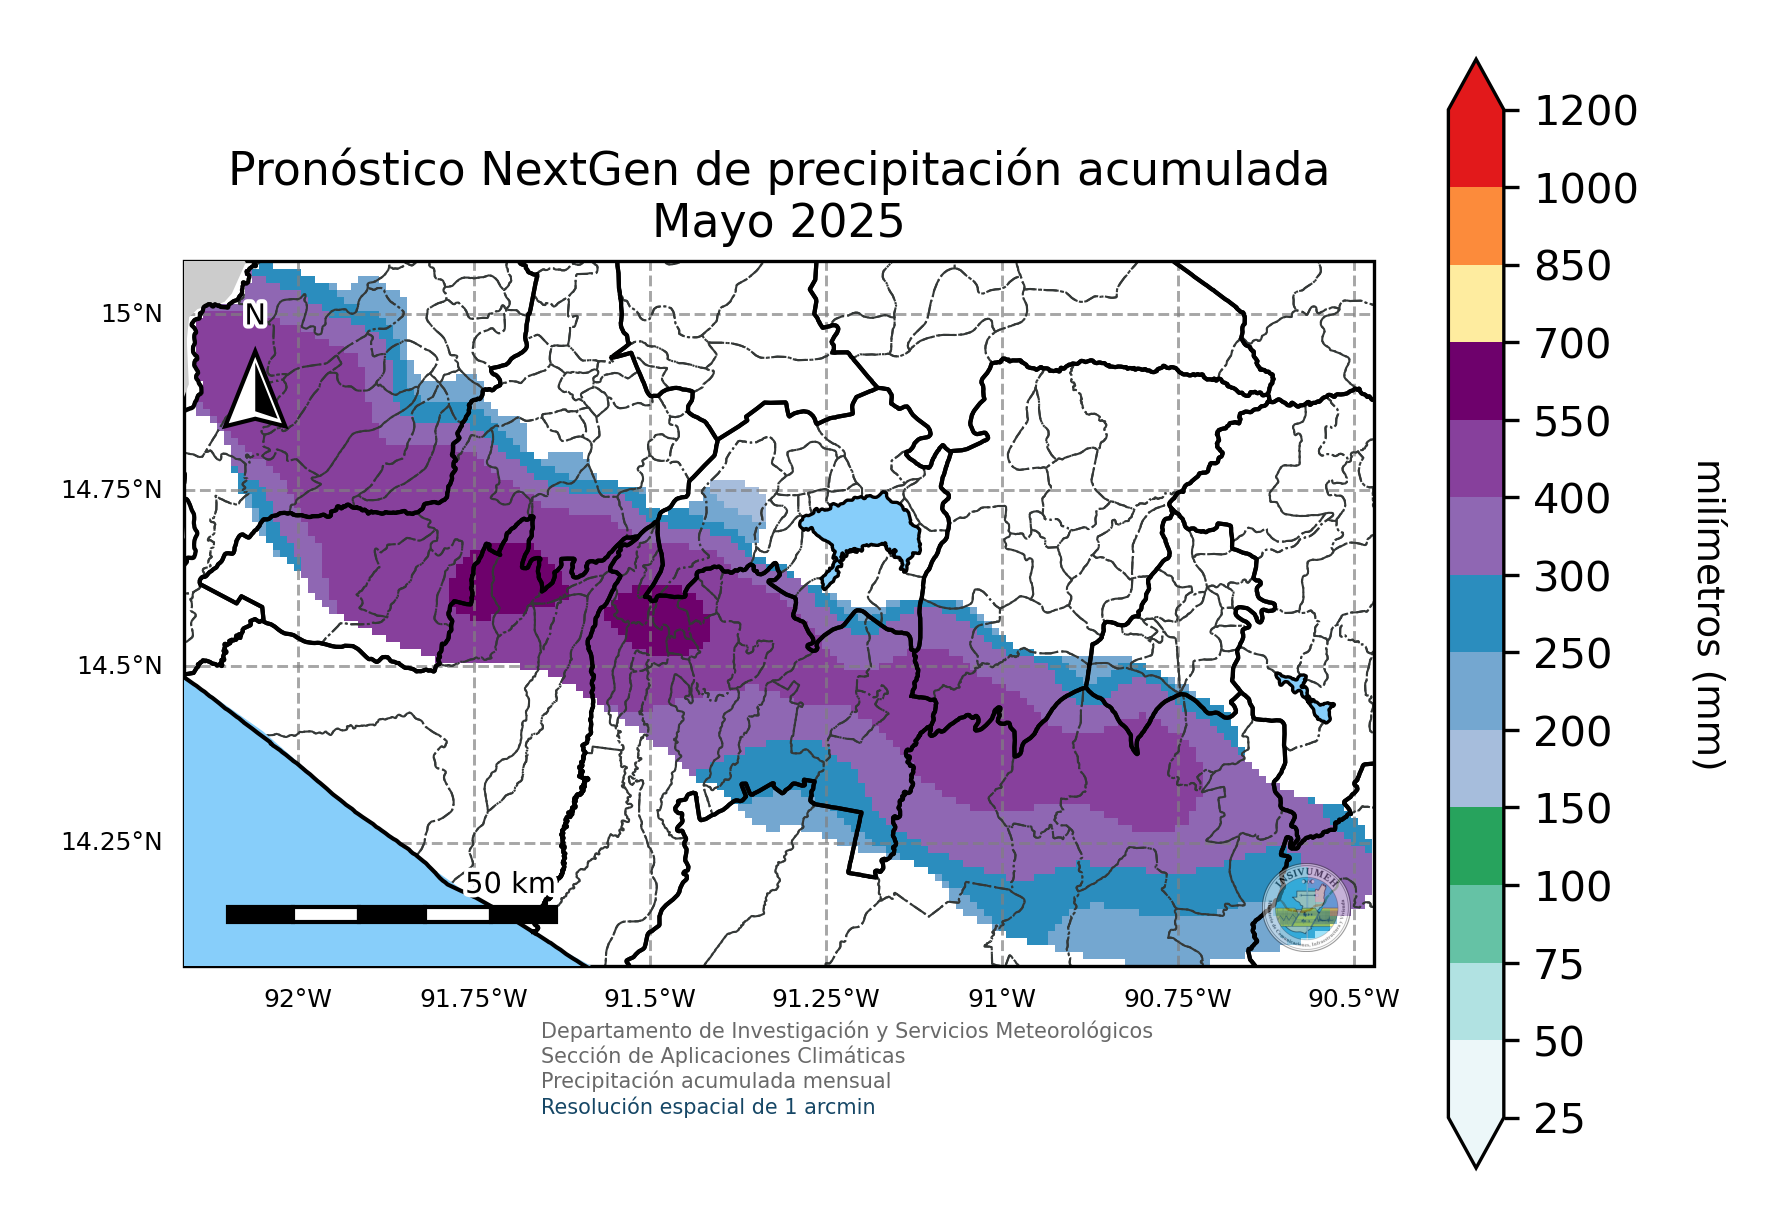
\includegraphics[width=\textwidth]{Informe/resultados/pronósticosNextGen/Pronóstico_NextGen_5_2025_Boca Costa_03.png}
	\end{subfigure}
	
	\vspace{-0.5em}
	
	\begin{subfigure}[b]{0.55\textwidth}
		\centering
		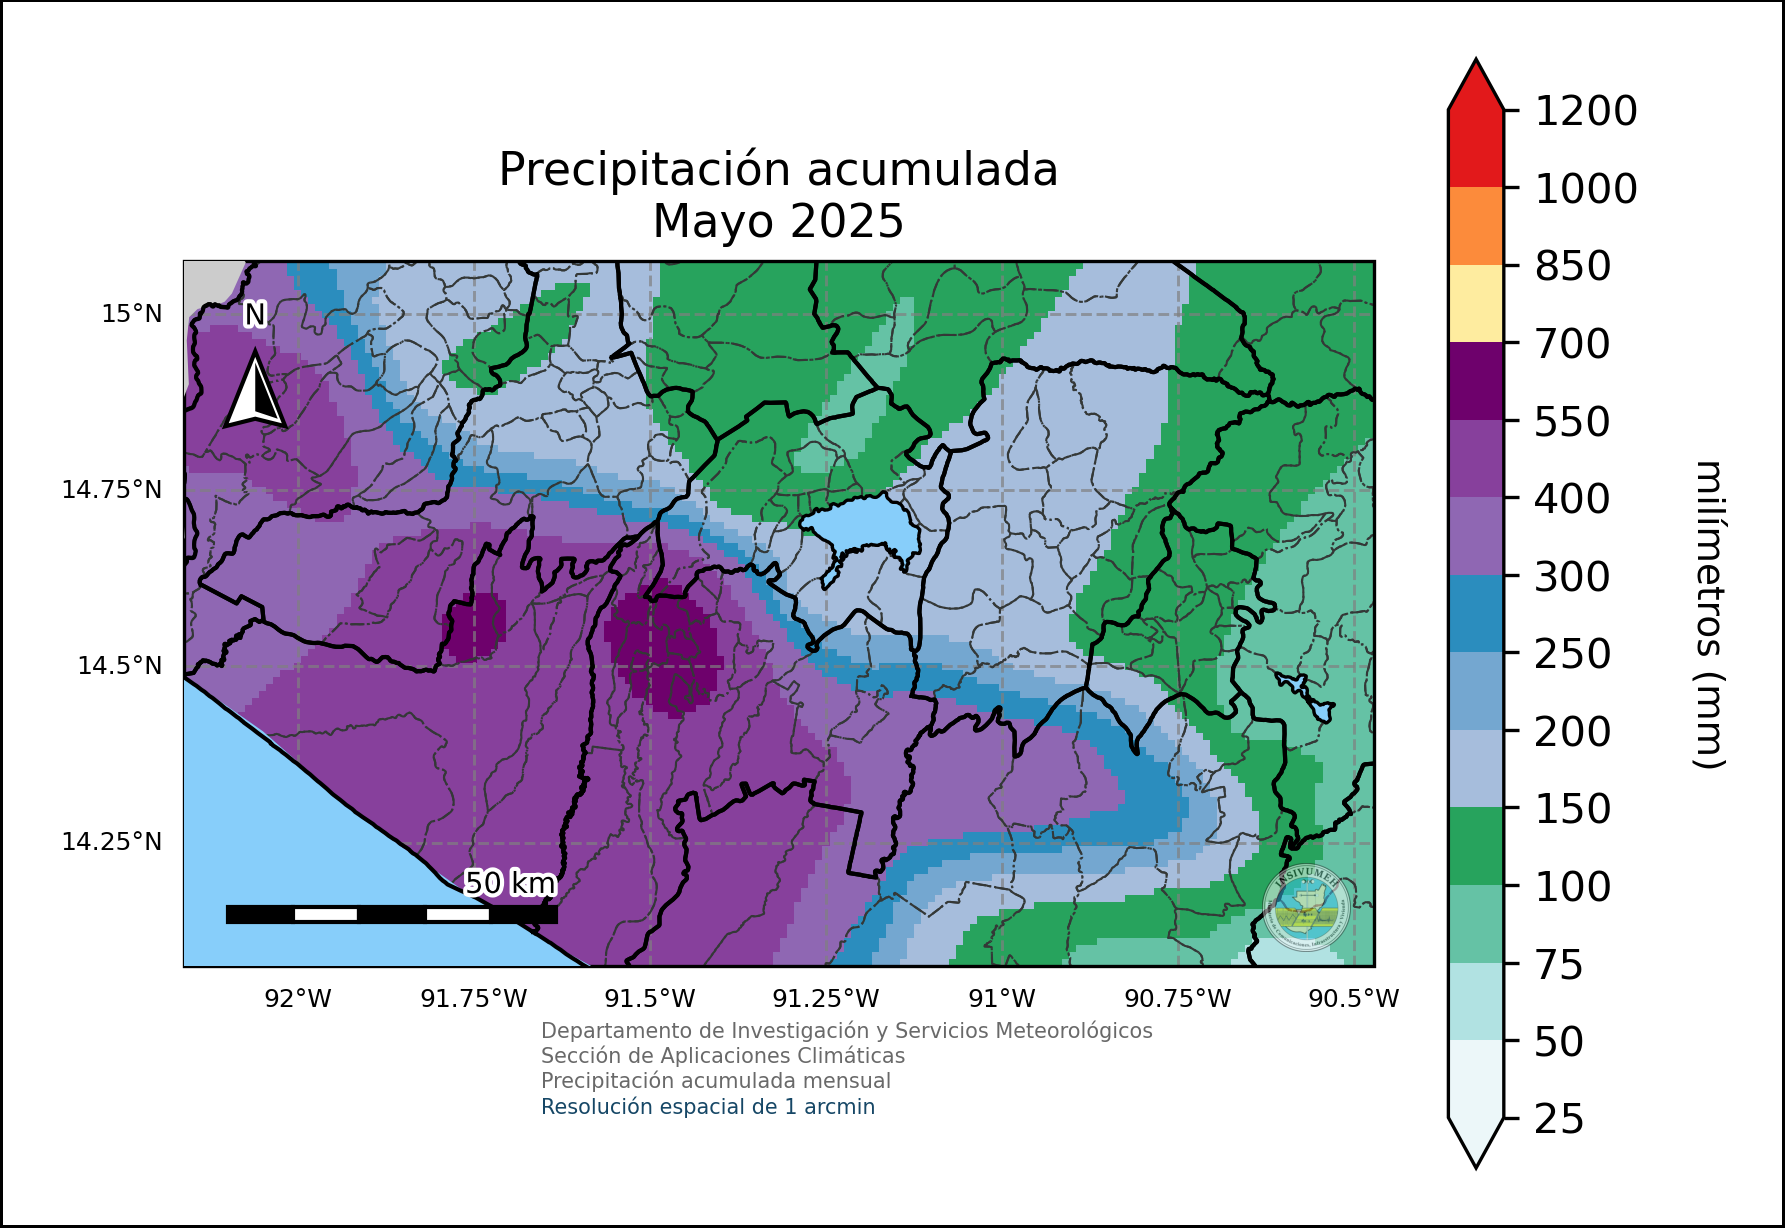
\includegraphics[width=\textwidth]{Informe/resultados/precipitación/Precipitación_5_2025_Boca Costa_03.png}
	\end{subfigure}
	
	\vspace{0.7em}
	
	% ==================================================
	% JUNIO
	% ==================================================
	
	\textbf{Junio 2025}
	
	\vspace{0.2em}
	
	\begin{subfigure}[b]{0.45\textwidth}
		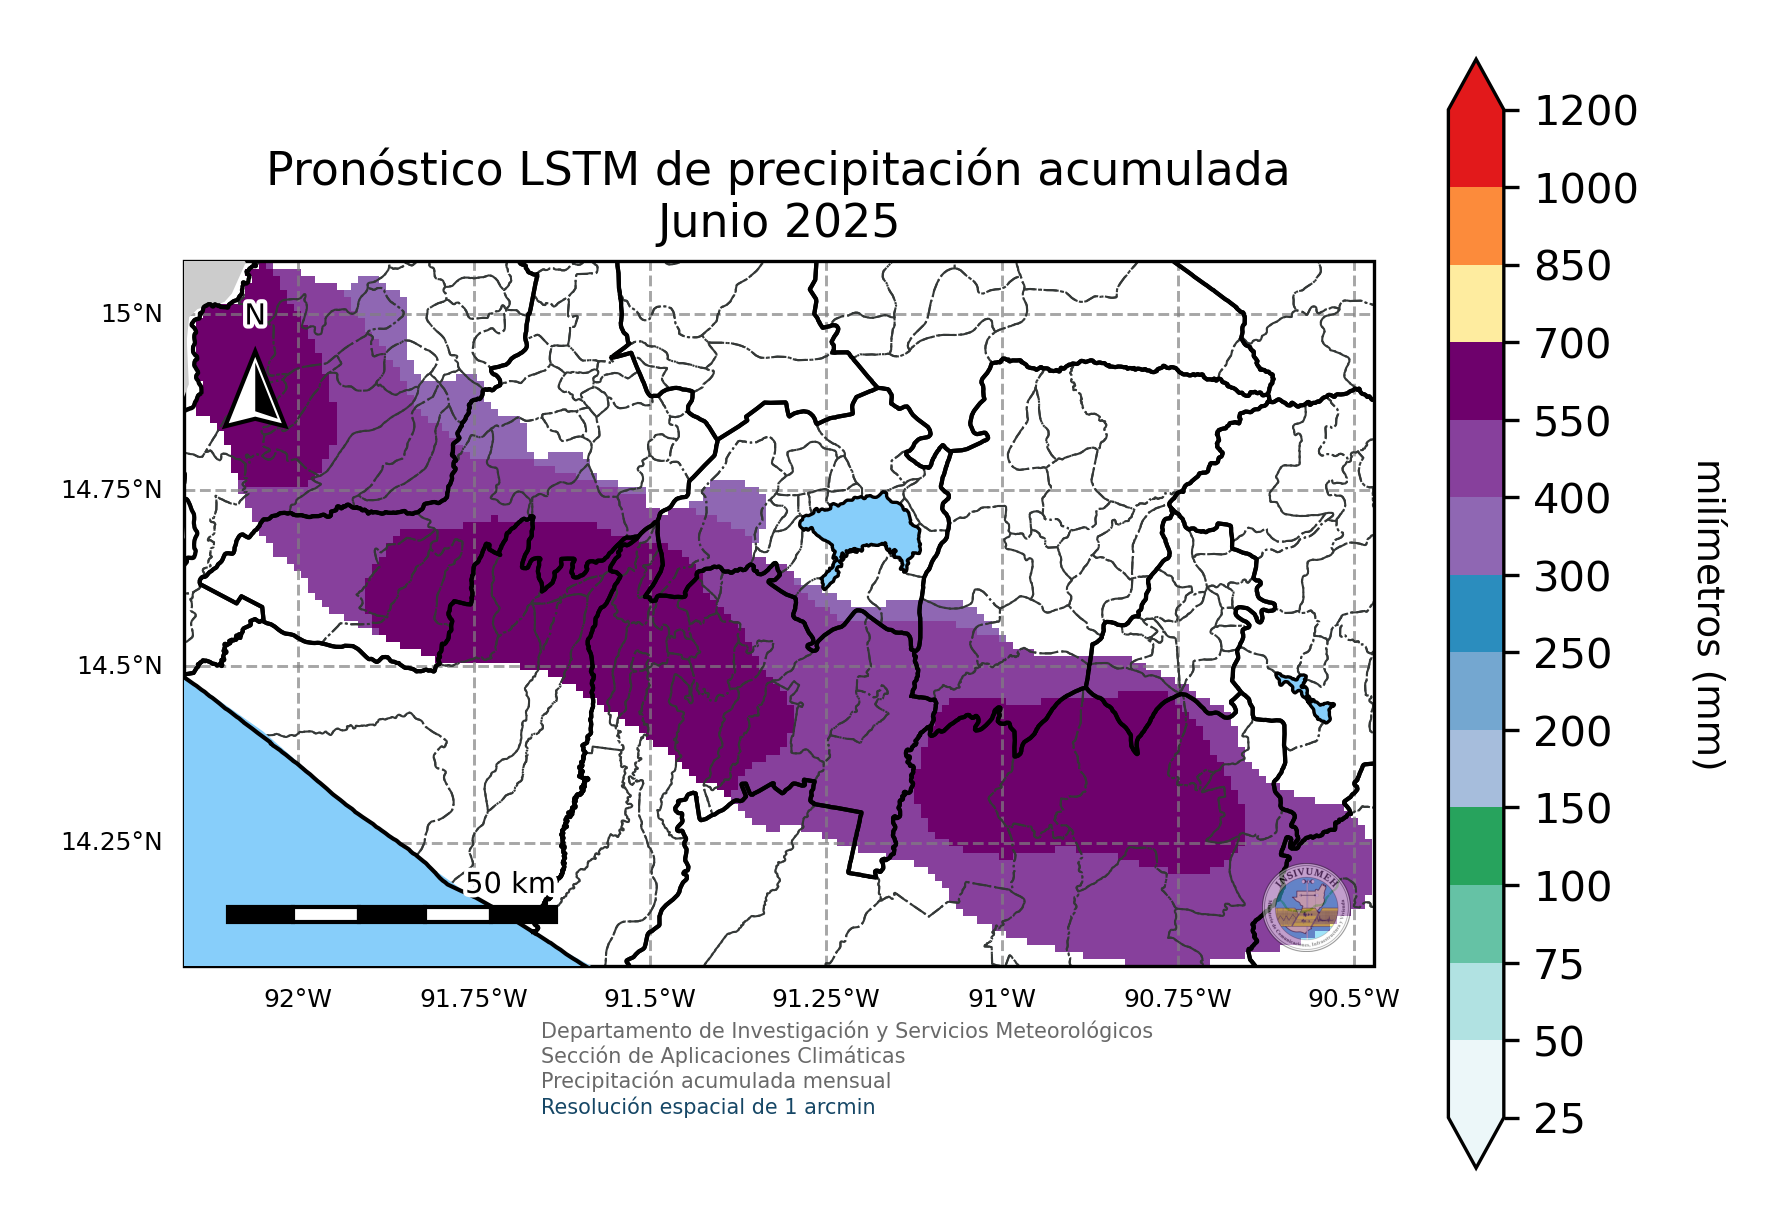
\includegraphics[width=\textwidth]{Informe/resultados/pronósticosLSTM/Pronóstico_LSTM_6_2025_Boca Costa_03.png}
	\end{subfigure}
	\hfill
	\begin{subfigure}[b]{0.45\textwidth}
		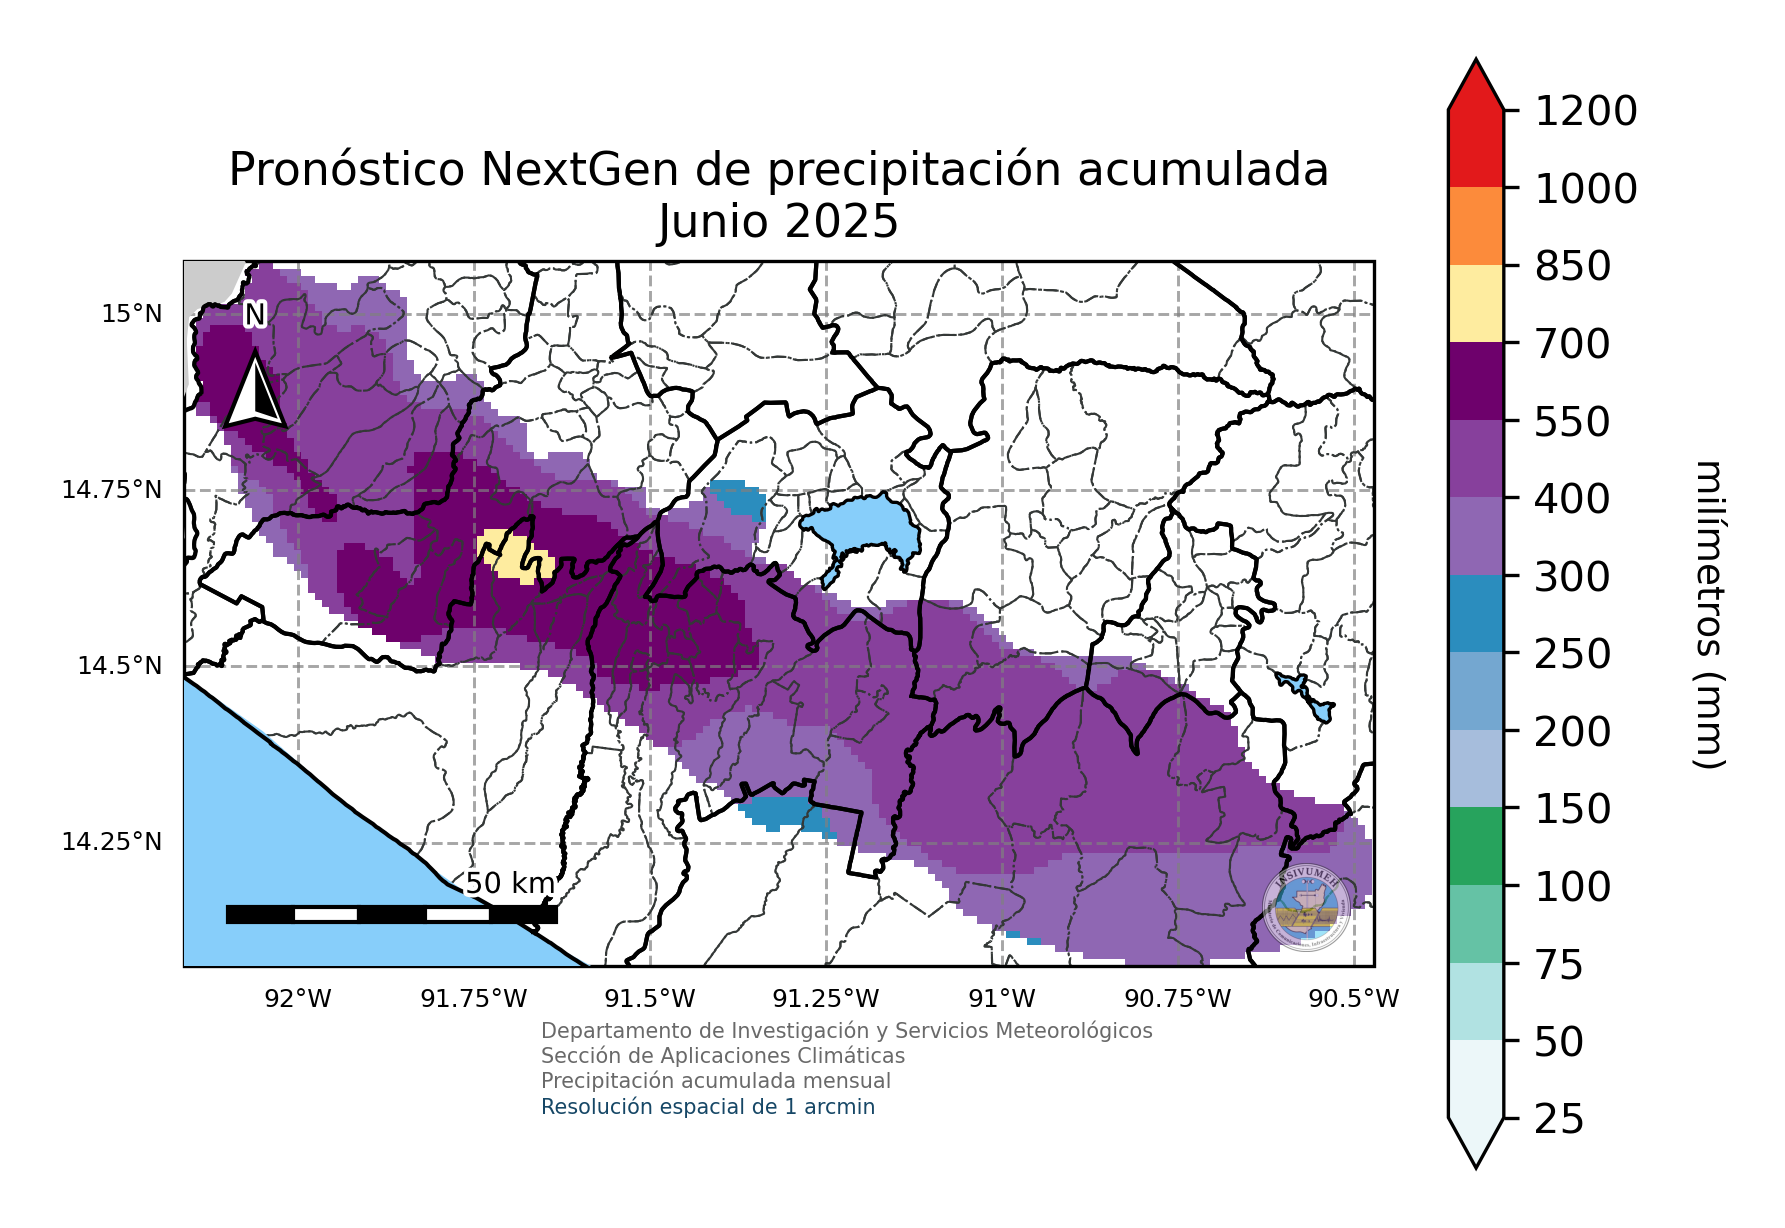
\includegraphics[width=\textwidth]{Informe/resultados/pronósticosNextGen/Pronóstico_NextGen_6_2025_Boca Costa_03.png}
	\end{subfigure}
	
	\vspace{-0.5em}
	
	\begin{subfigure}[b]{0.55\textwidth}
		\centering
		
\includegraphics[width=\textwidth]{Informe/resultados/precipitación/Precipitación_6_2025_Boca Costa_03.png}
	\end{subfigure}
	```
	
\end{figure}

\begin{figure}[!htbp]
	\centering
	% ==================================================
	% JULIO
	% ==================================================
	
	\textbf{Julio 2025}
	
	\vspace{0.2em}
	
	\begin{subfigure}[b]{0.45\textwidth}
		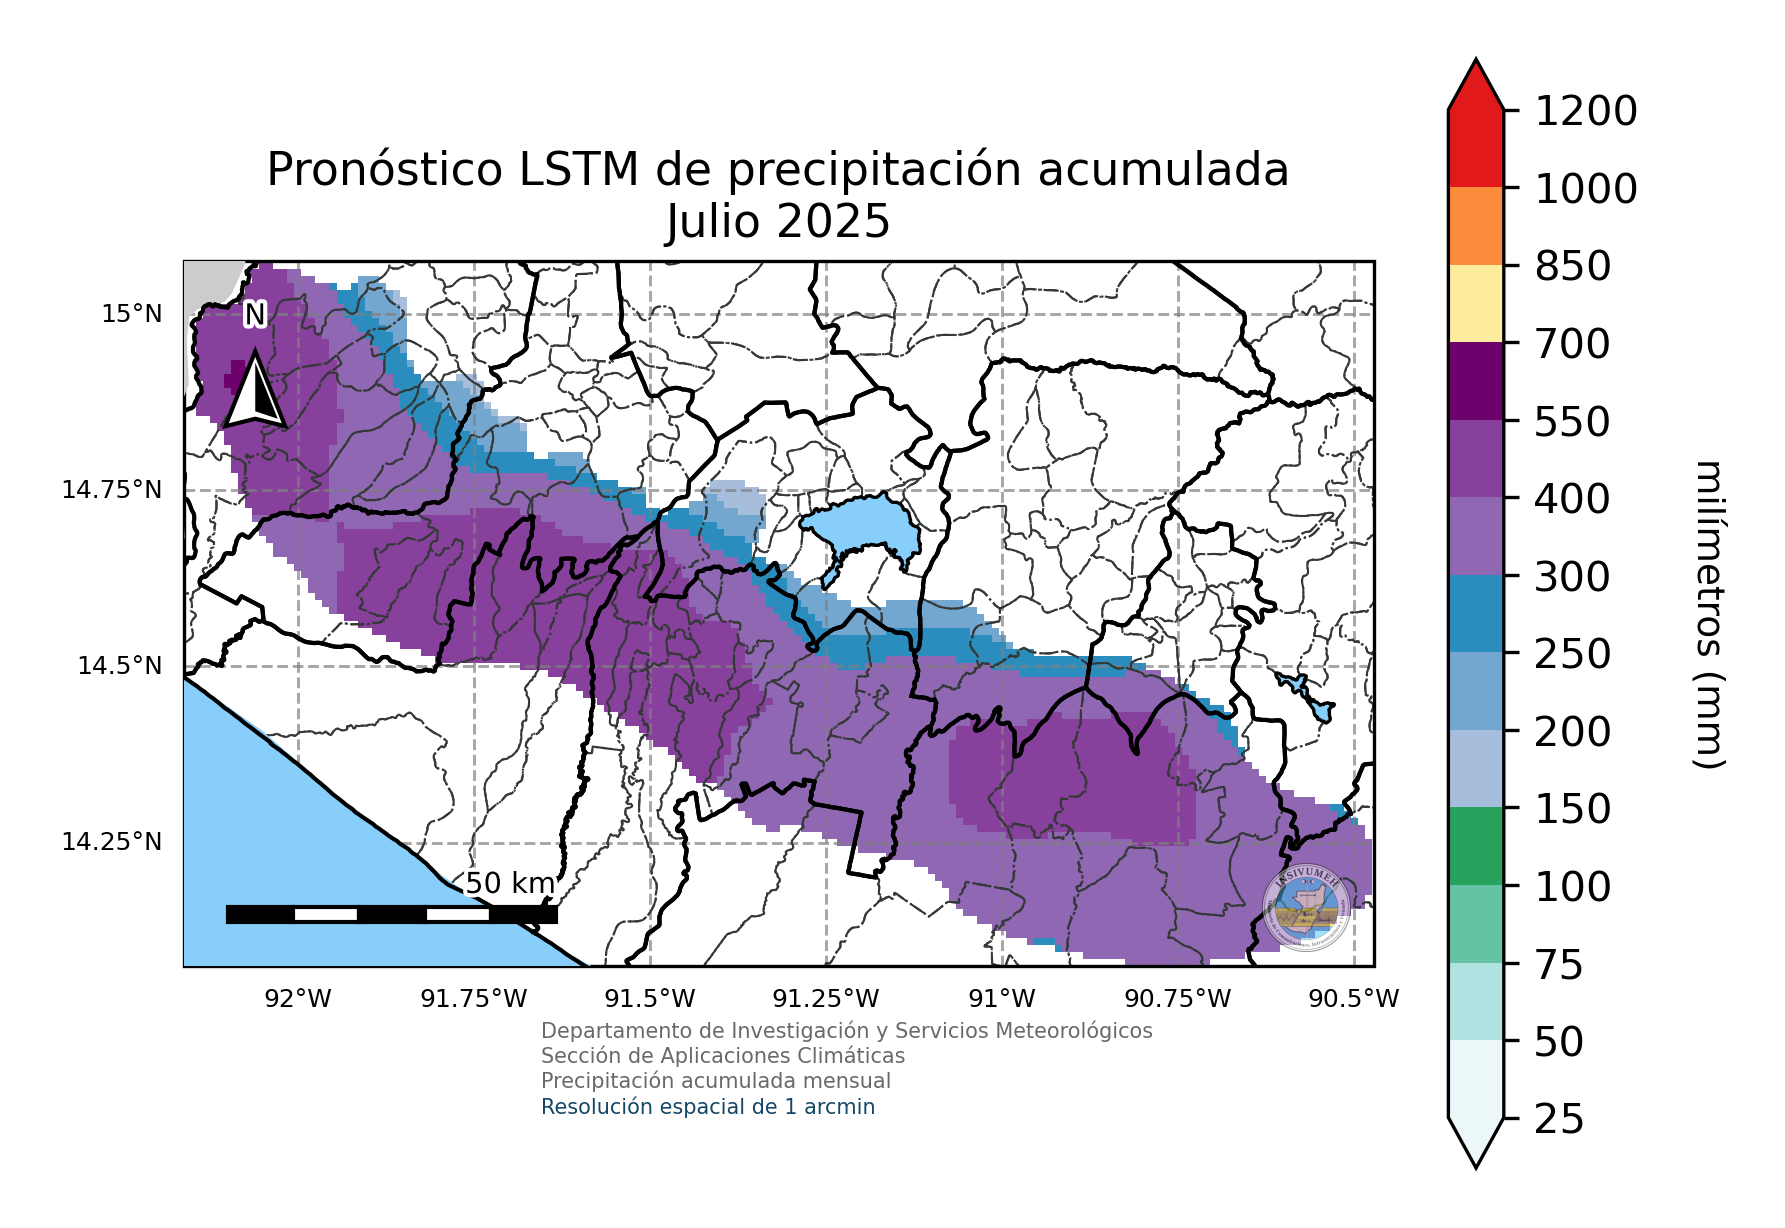
\includegraphics[width=\textwidth]{Informe/resultados/pronósticosLSTM/Pronóstico_LSTM_7_2025_Boca Costa_03.png}
	\end{subfigure}
	\hfill
	\begin{subfigure}[b]{0.45\textwidth}
		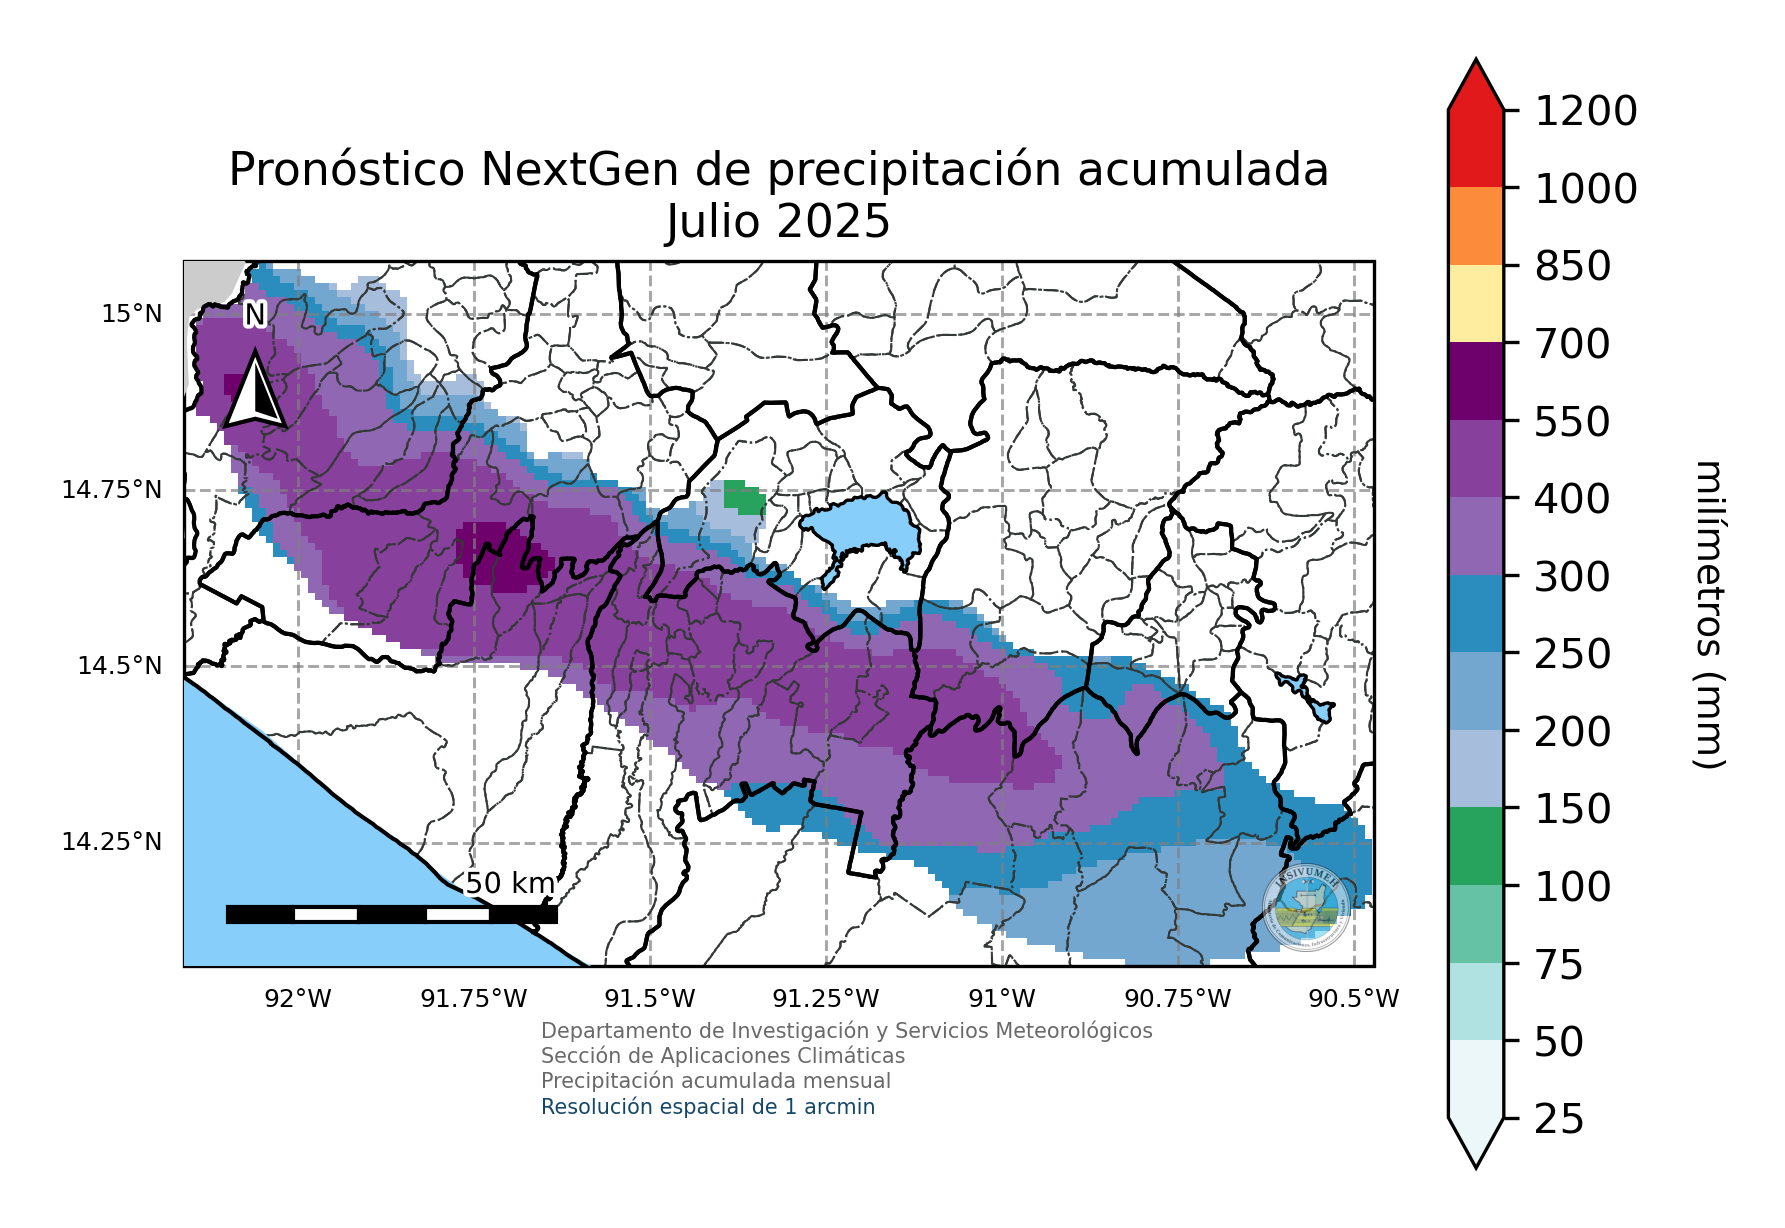
\includegraphics[width=\textwidth]{Informe/resultados/pronósticosNextGen/Pronóstico_NextGen_7_2025_Boca Costa_03.png}
	\end{subfigure}
	
	\vspace{-0.5em}
	
	\begin{subfigure}[b]{0.55\textwidth}
		\centering
		
\includegraphics[width=\textwidth]{Informe/resultados/precipitación/Precipitación_7_2025_Boca Costa_03.png}
	\end{subfigure}
	
	\vspace{0.7em}
	
	% ==================================================
	% AGOSTO
	% ==================================================
	
	\textbf{Agosto 2025}
	
	\vspace{0.2em}
	
	\begin{subfigure}[b]{0.45\textwidth}
		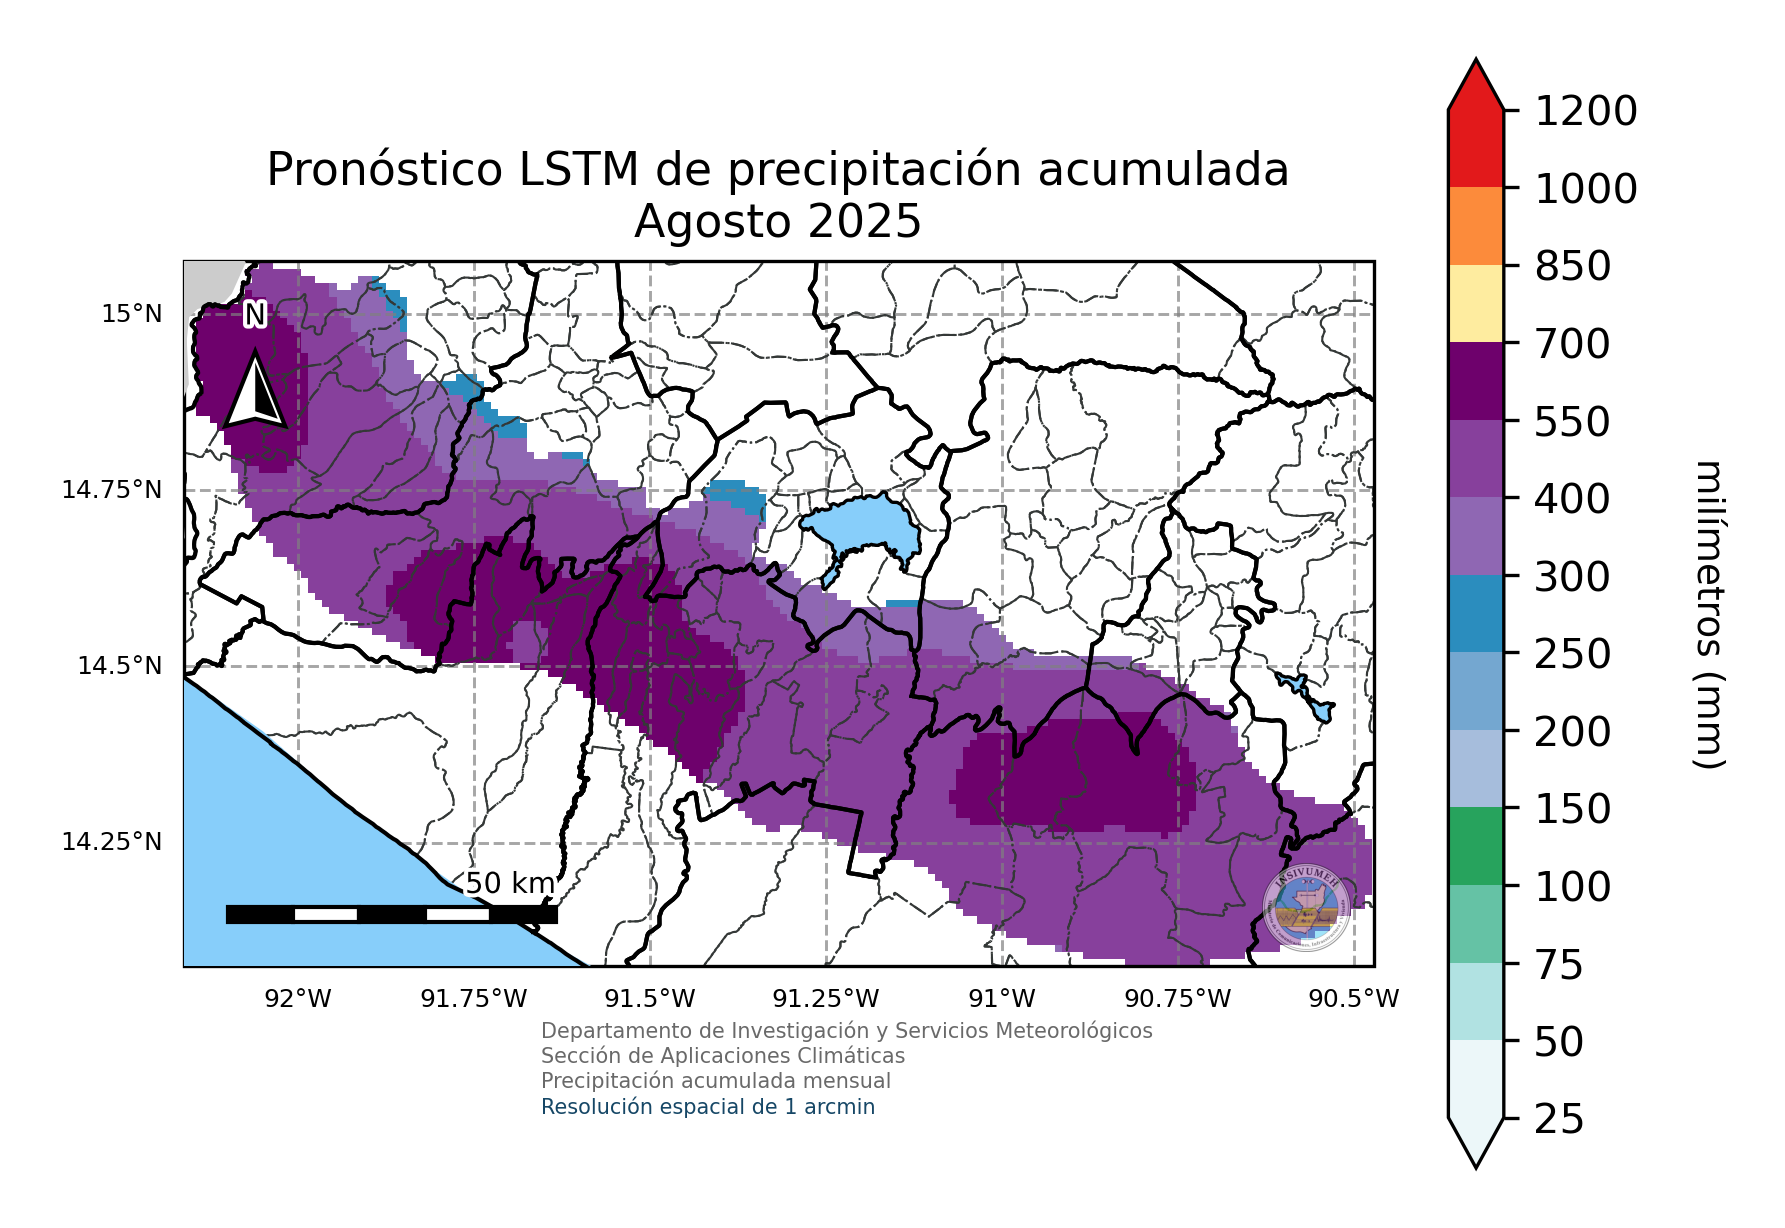
\includegraphics[width=\textwidth]{Informe/resultados/pronósticosLSTM/Pronóstico_LSTM_8_2025_Boca Costa_03.png}
	\end{subfigure}
	\hfill
	\begin{subfigure}[b]{0.45\textwidth}
		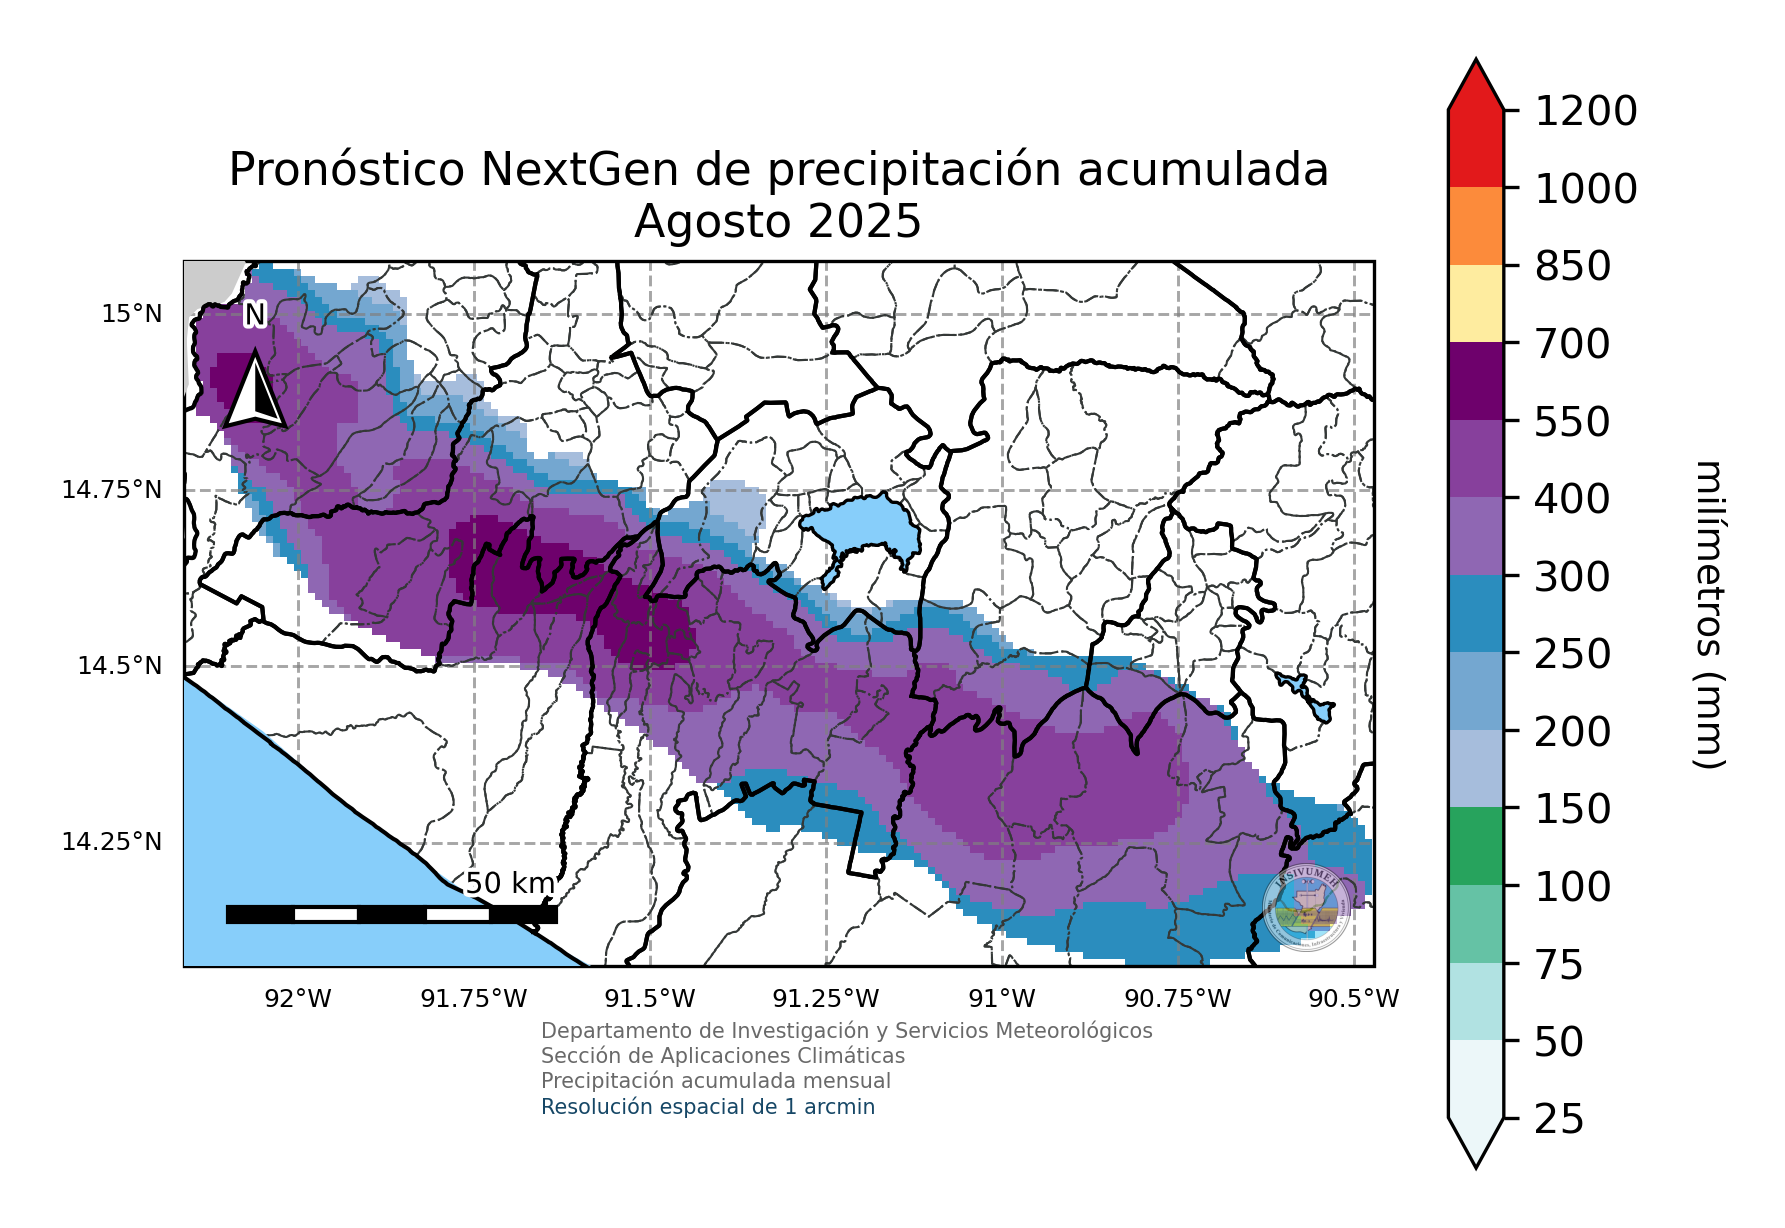
\includegraphics[width=\textwidth]{Informe/resultados/pronósticosNextGen/Pronóstico_NextGen_8_2025_Boca Costa_03.png}
	\end{subfigure}
	
	\vspace{-0.5em}
	
	\begin{subfigure}[b]{0.55\textwidth}
		\centering
		
\includegraphics[width=\textwidth]{Informe/resultados/precipitación/Precipitación_8_2025_Boca Costa_03.png}
	\end{subfigure}
	```
	
\end{figure}

\begin{figure}[!htbp]
	\centering
	% ==================================================
	% SEPTIEMBRE
	% ==================================================
	
	\textbf{Septiembre 2025}
	
	\vspace{0.2em}
	
	\begin{subfigure}[b]{0.45\textwidth}
		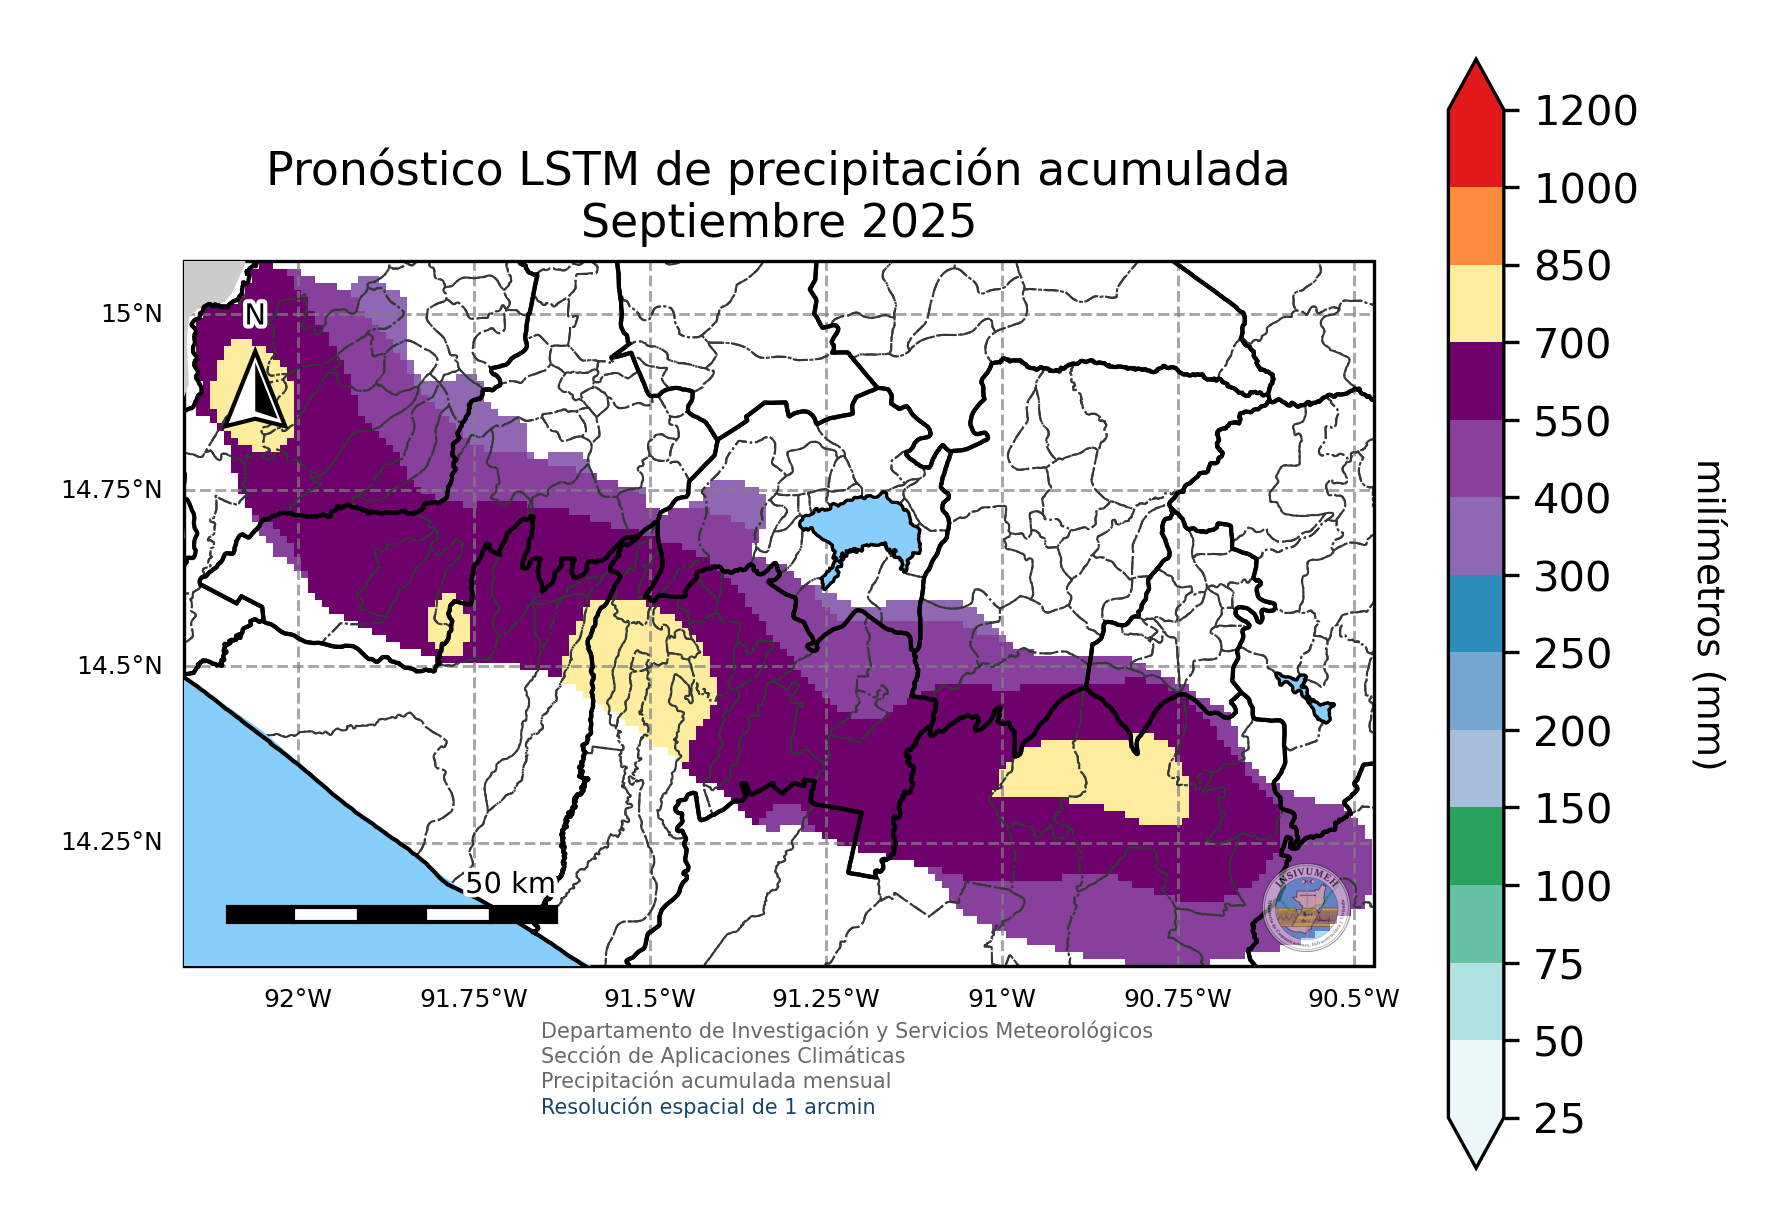
\includegraphics[width=\textwidth]{Informe/resultados/pronósticosLSTM/Pronóstico_LSTM_9_2025_Boca Costa_03.png}
	\end{subfigure}
	\hfill
	\begin{subfigure}[b]{0.45\textwidth}
		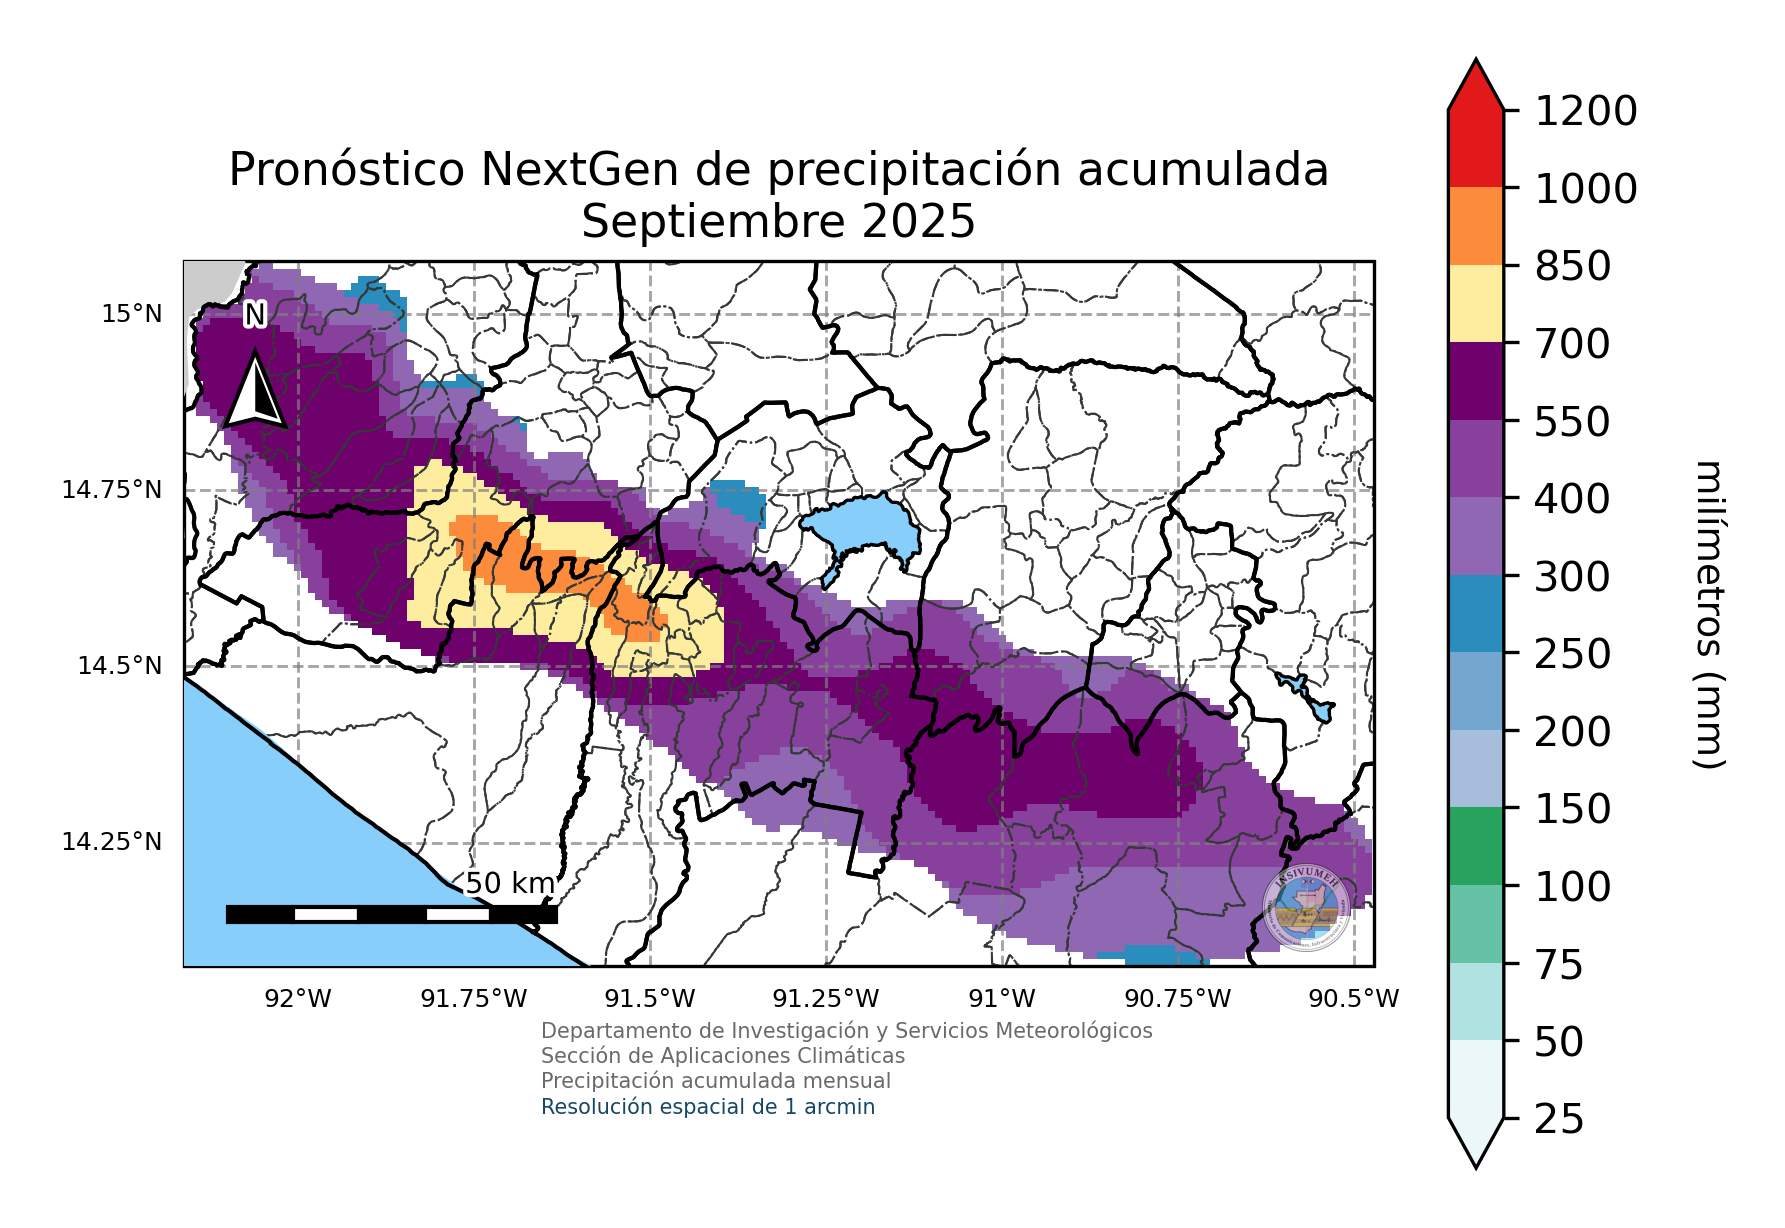
\includegraphics[width=\textwidth]{Informe/resultados/pronósticosNextGen/Pronóstico_NextGen_9_2025_Boca Costa_03.png}
	\end{subfigure}
	
	\vspace{-0.5em}
	
	\begin{subfigure}[b]{0.55\textwidth}
		\centering
		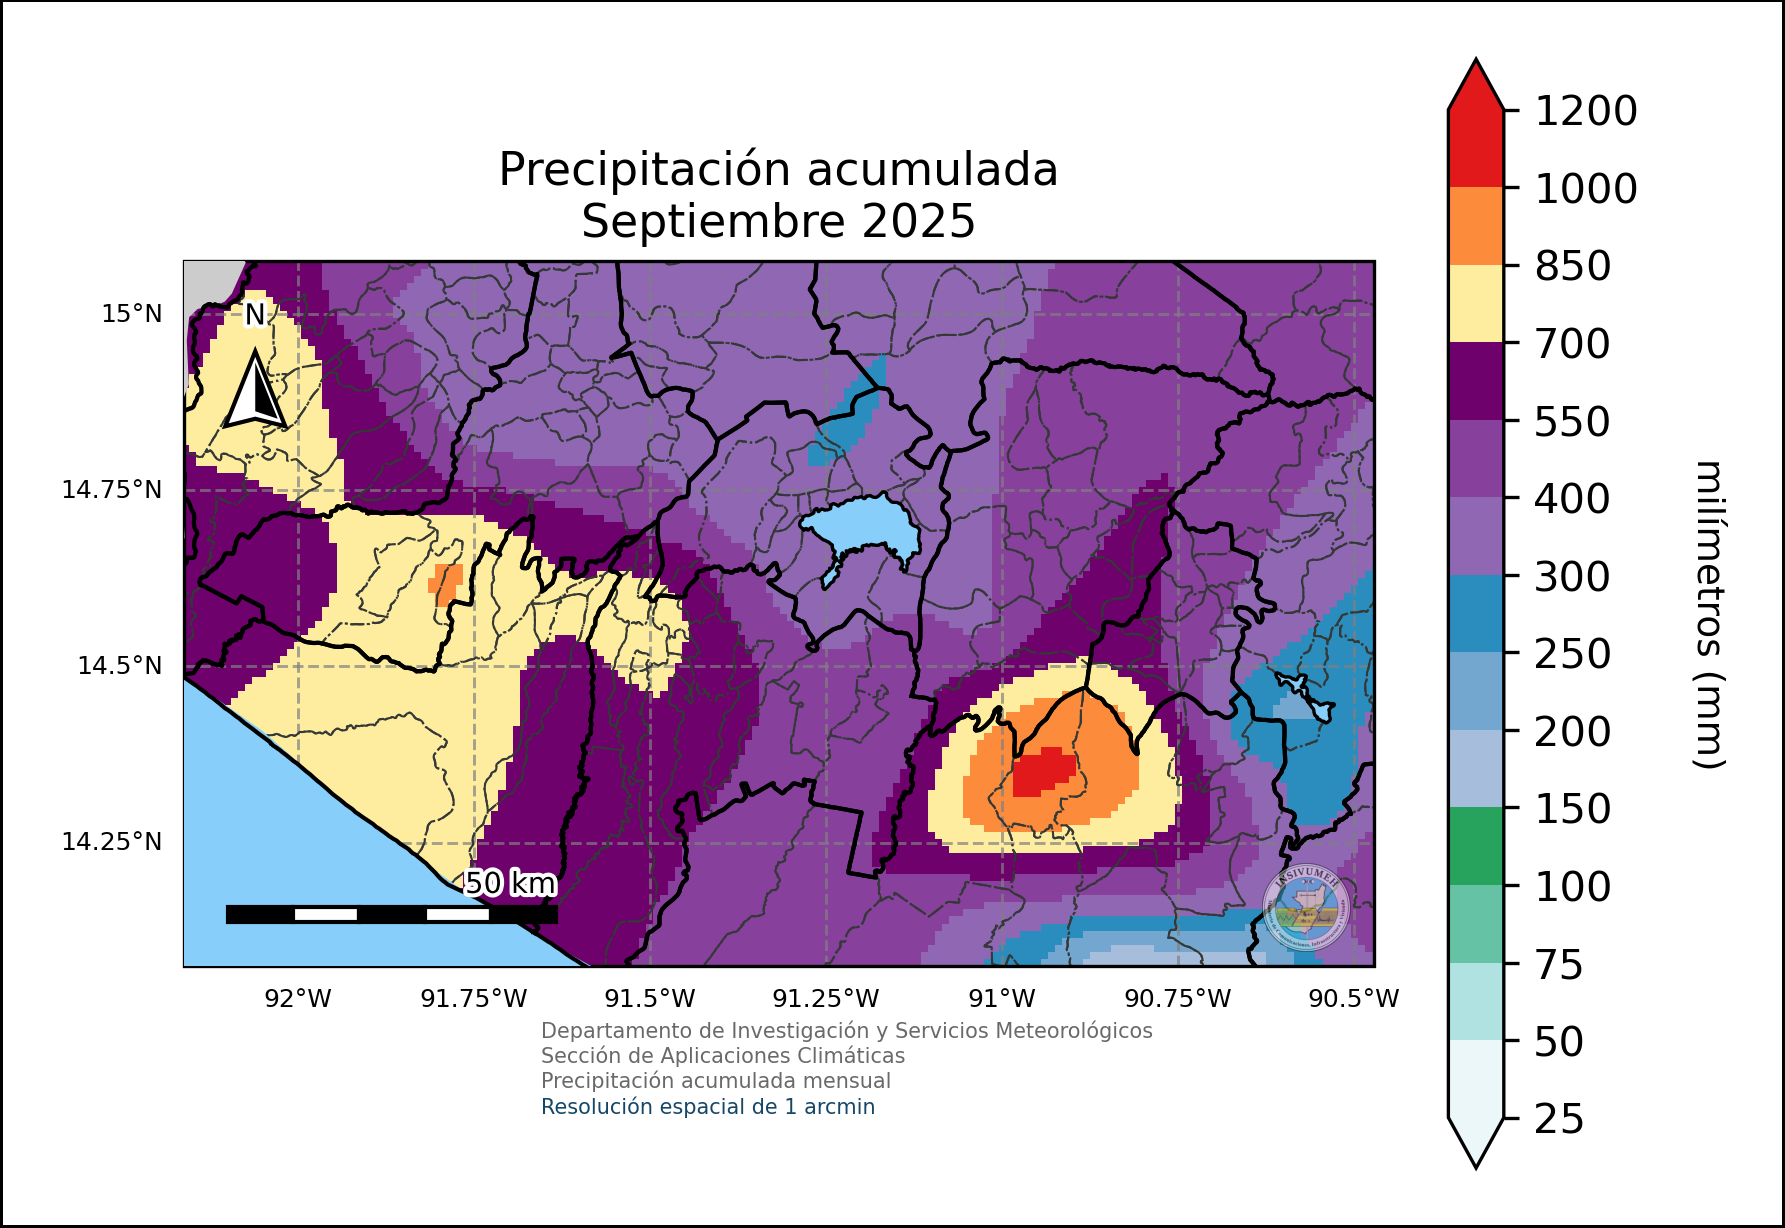
\includegraphics[width=\textwidth]{Informe/resultados/precipitación/Precipitación_9_2025_Boca Costa_03.png}
	\end{subfigure}
	
	\vspace{0.7em}
	
	% ==================================================
	% OCTUBRE
	% ==================================================
	
	\textbf{Octubre 2025}
	
	\vspace{0.2em}
	
	\begin{subfigure}[b]{0.45\textwidth}
		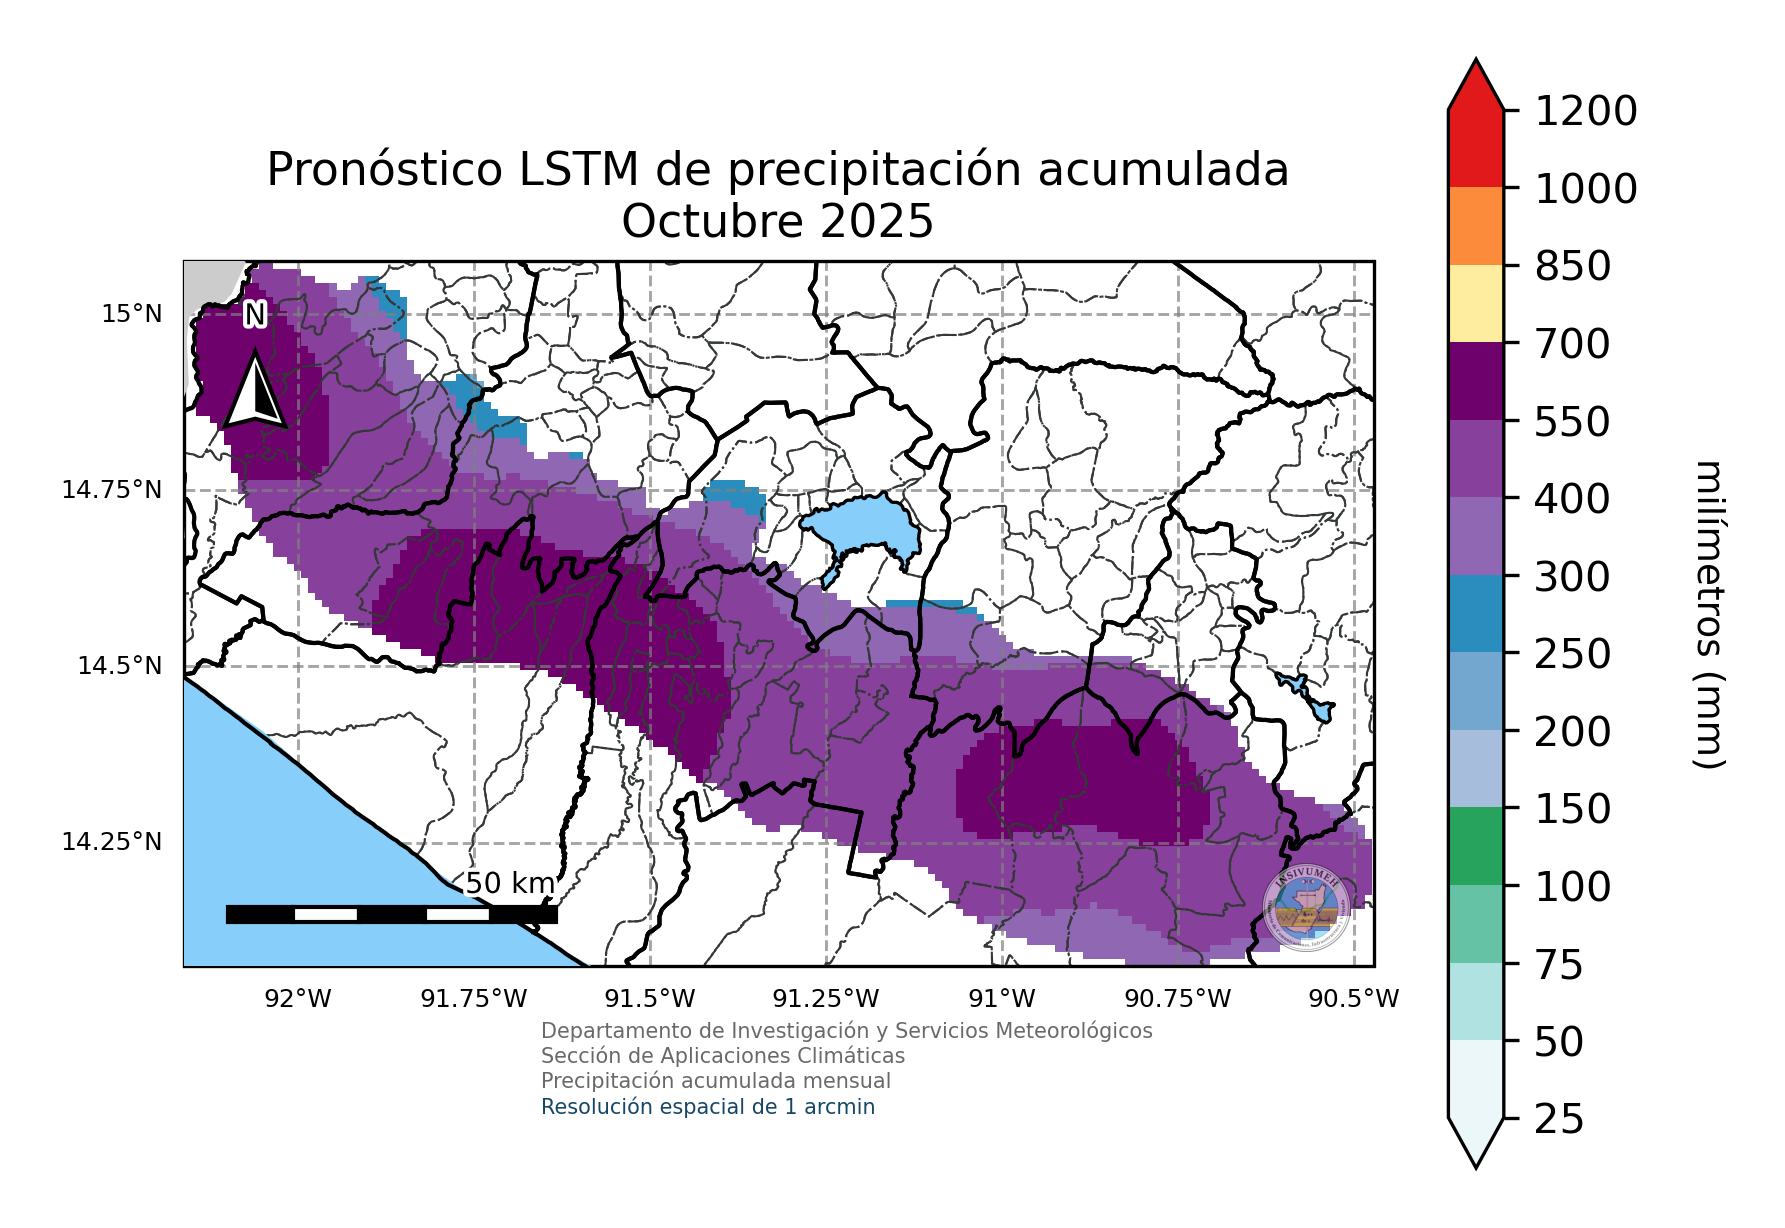
\includegraphics[width=\textwidth]{Informe/resultados/pronósticosLSTM/Pronóstico_LSTM_10_2025_Boca Costa_03.png}
	\end{subfigure}
	\hfill
	\begin{subfigure}[b]{0.45\textwidth}
		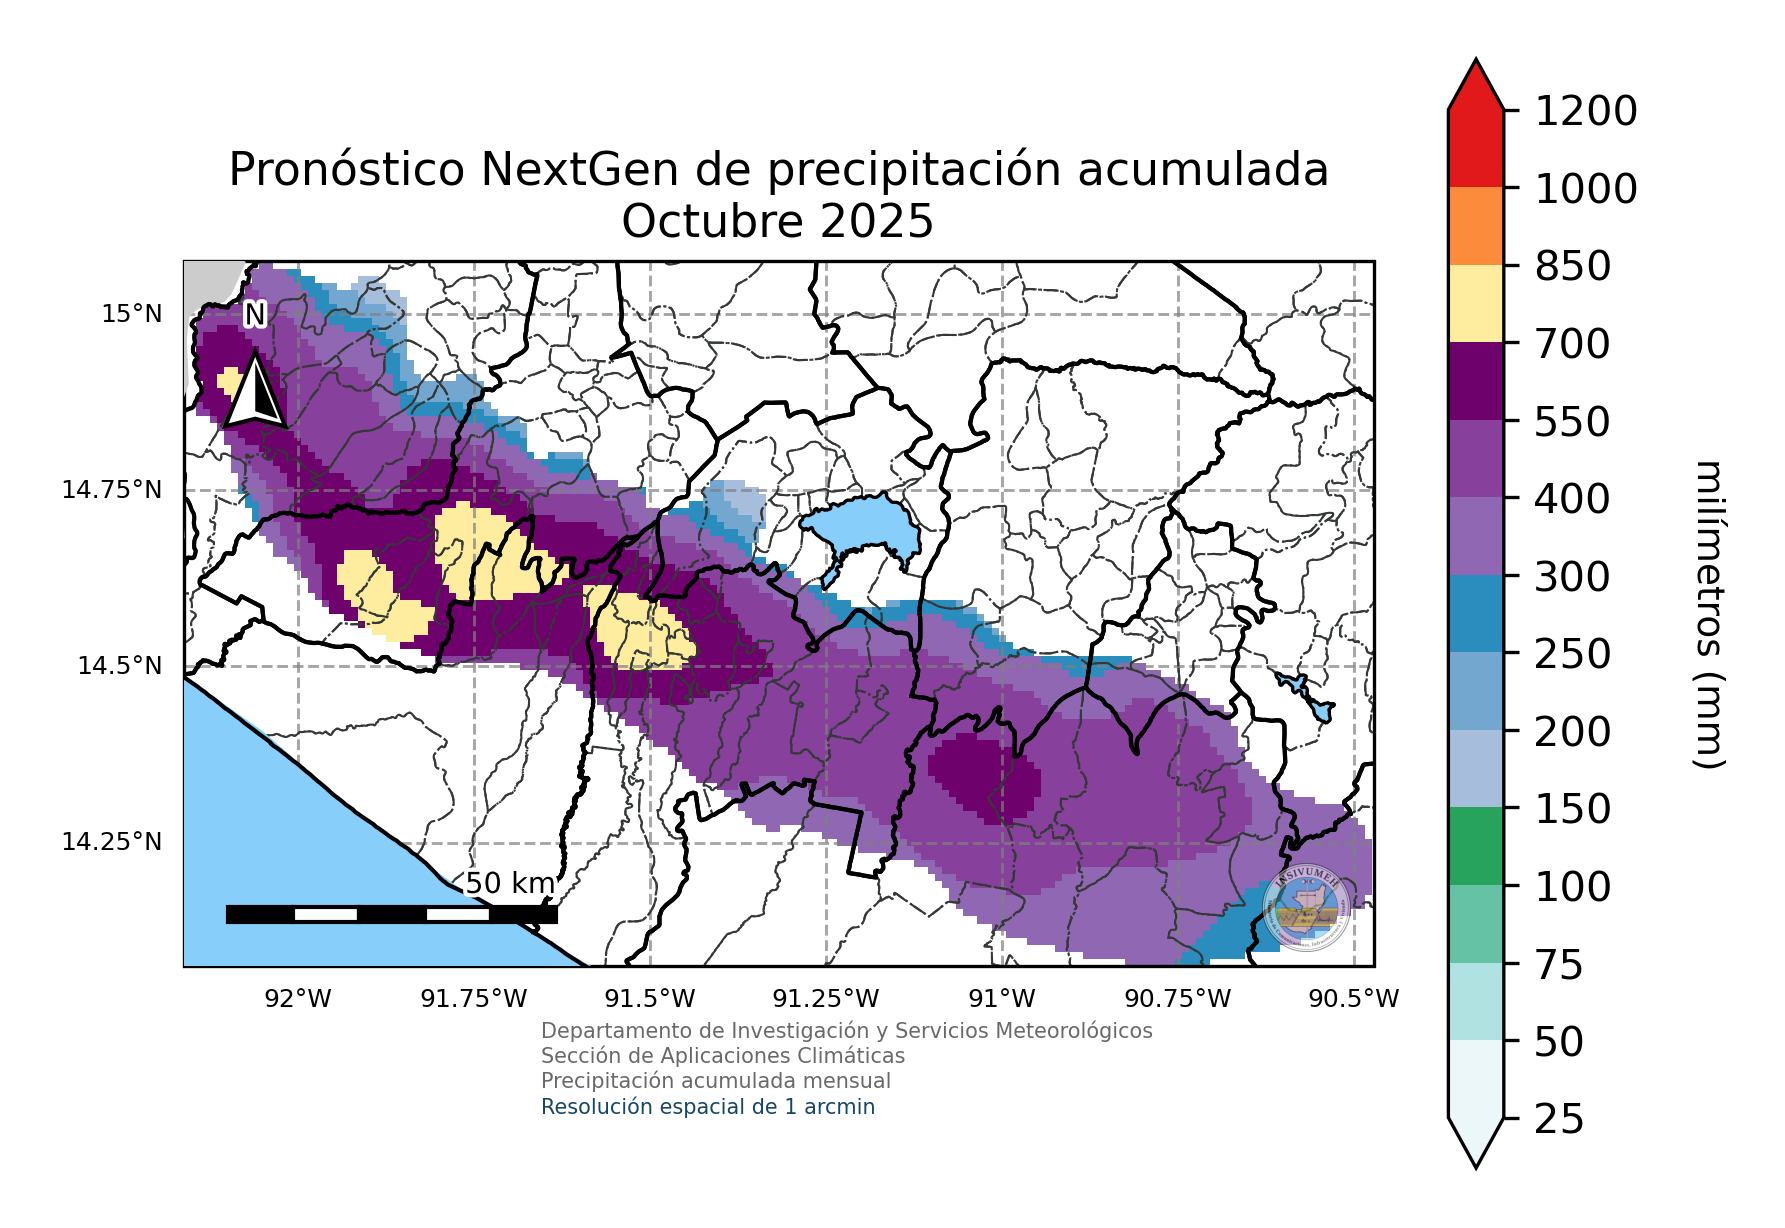
\includegraphics[width=\textwidth]{Informe/resultados/pronósticosNextGen/Pronóstico_NextGen_10_2025_Boca Costa_03.png}
	\end{subfigure}
	
	\vspace{-0.5em}
	
	\begin{subfigure}[b]{0.55\textwidth}
		\centering
		
\includegraphics[width=\textwidth]{Informe/resultados/precipitación/Precipitación_10_2025_Boca Costa_03.png}
	\end{subfigure}
	```
	
\end{figure}

\begin{figure}[!htbp]
	\centering

	% ==================================================
	% NOVIEMBRE
	% ==================================================
	
	\textbf{Noviembre 2025}
	
	\vspace{0.2em}
	
	\begin{subfigure}[b]{0.45\textwidth}
		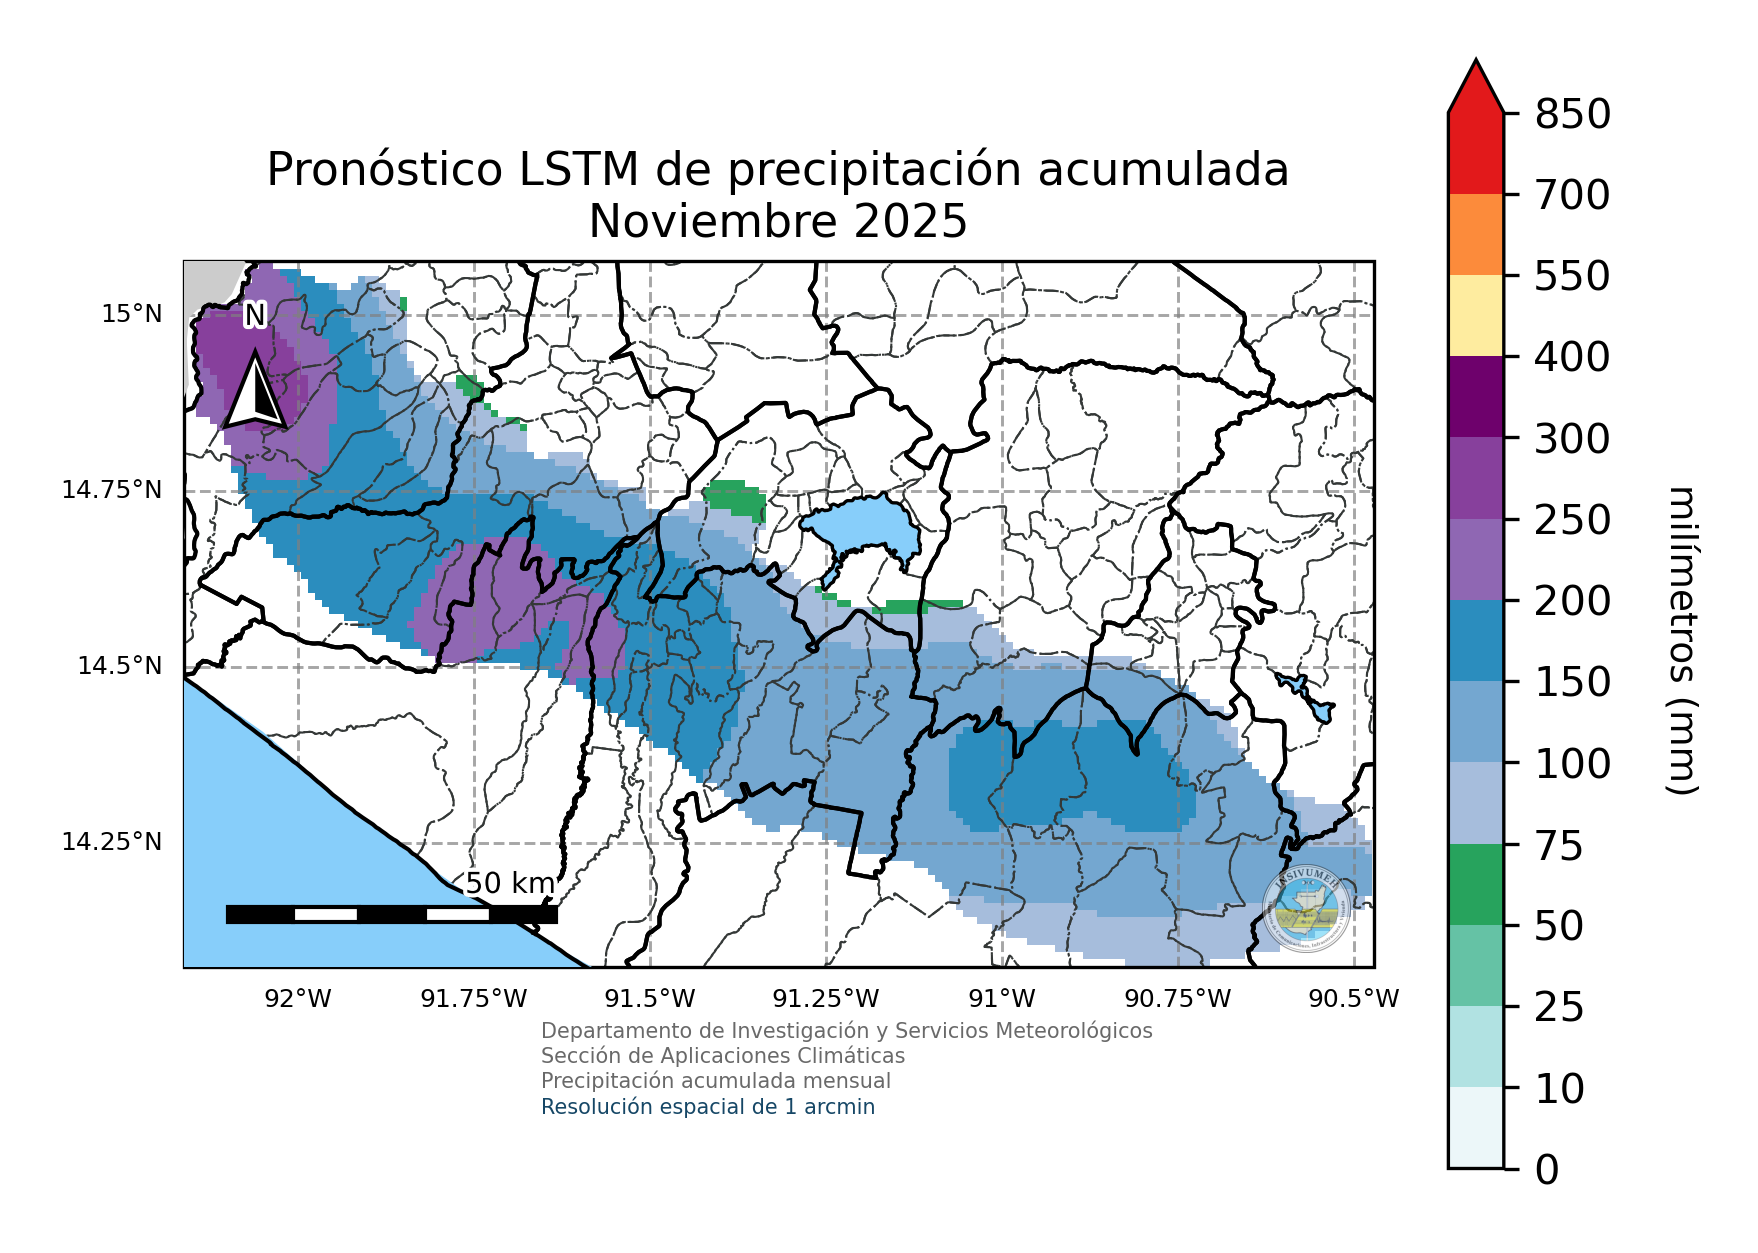
\includegraphics[width=\textwidth]{Informe/resultados/pronósticosLSTM/Pronóstico_LSTM_11_2025_Boca Costa_03.png}
	\end{subfigure}
	\hfill
	\begin{subfigure}[b]{0.45\textwidth}
		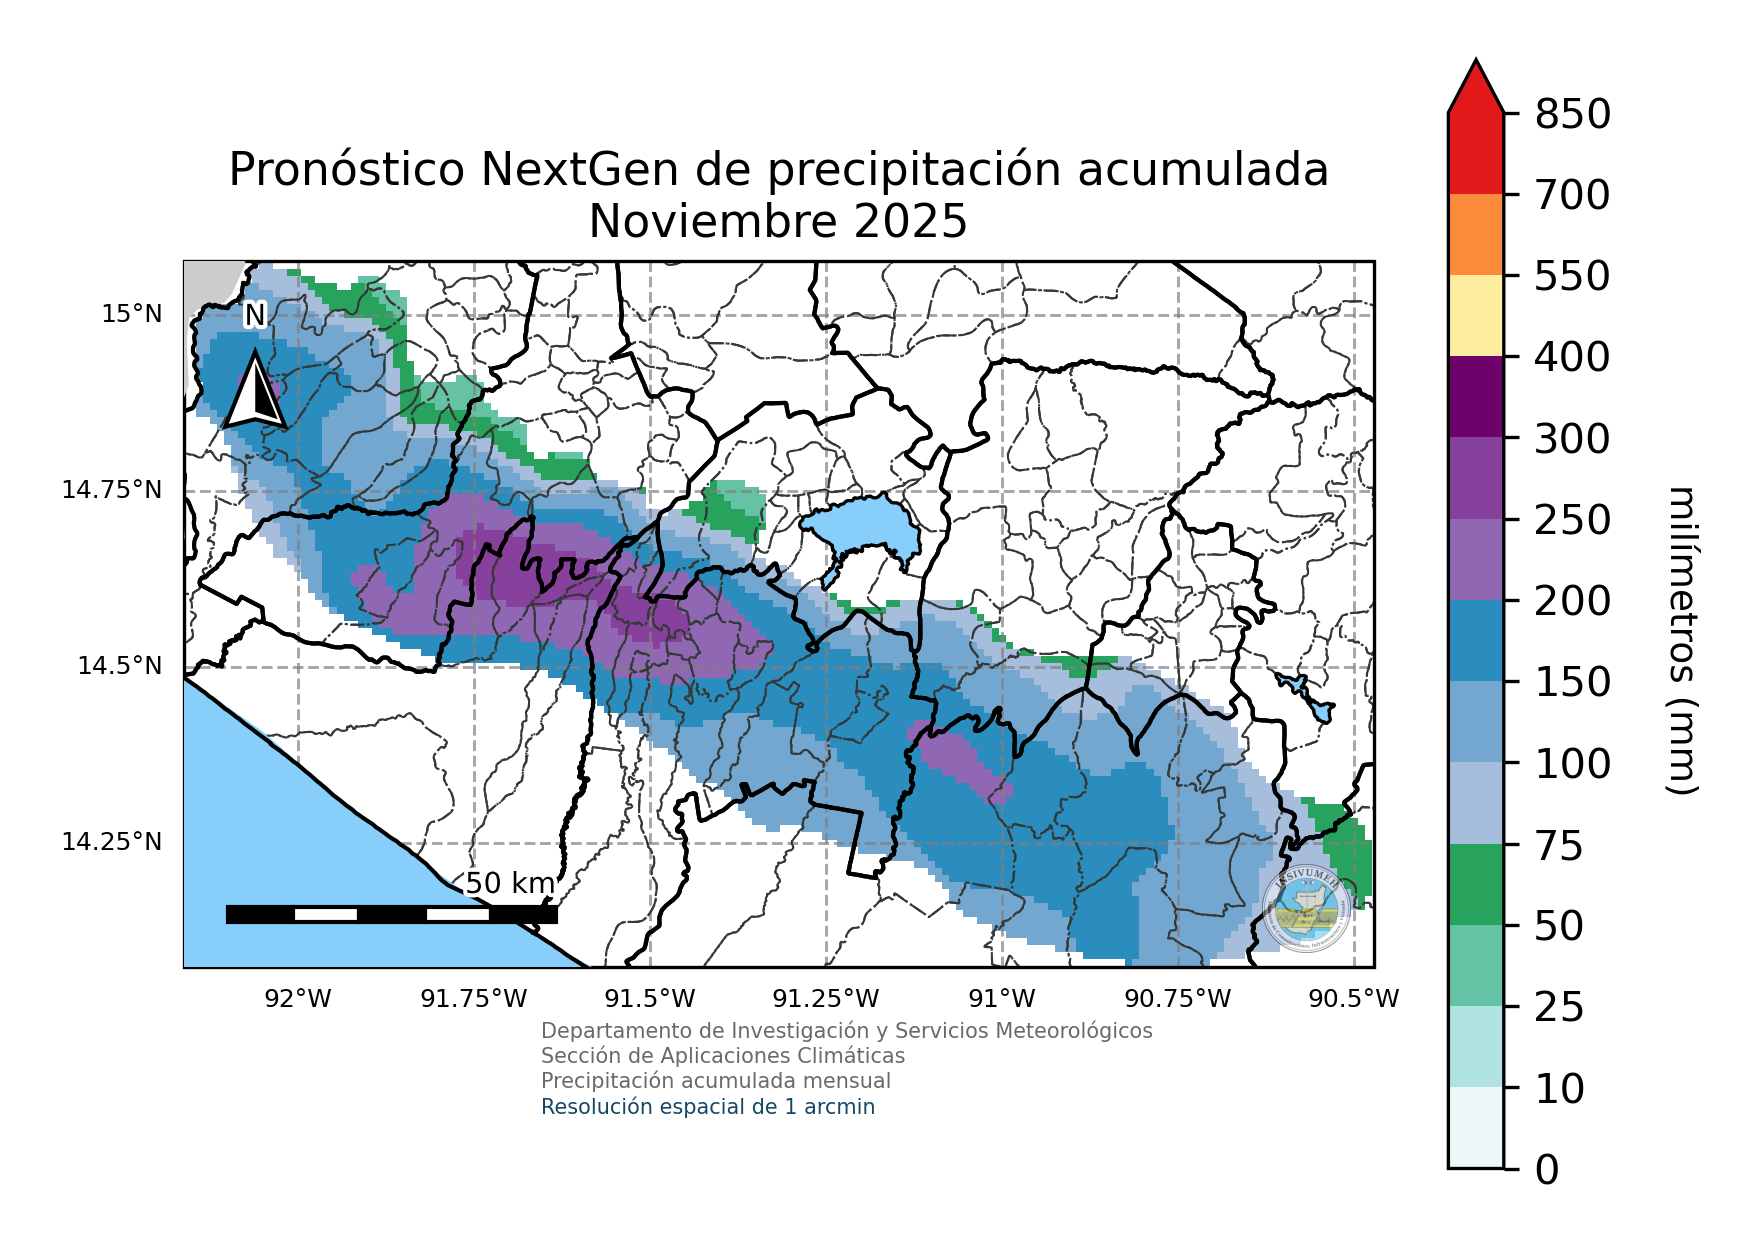
\includegraphics[width=\textwidth]{Informe/resultados/pronósticosNextGen/Pronóstico_NextGen_11_2025_Boca Costa_03.png}
	\end{subfigure}
	
	\vspace{-0.5em}
	
	\begin{subfigure}[b]{0.55\textwidth}
		\centering
		
\includegraphics[width=\textwidth]{Informe/resultados/precipitación/Precipitación_11_2025_Boca Costa_03.png}
	\end{subfigure}
	
	\vspace{0.7em}
	
	% ==================================================
	% DICIEMBRE
	% ==================================================
	
	\textbf{Diciembre 2025}
	
	\vspace{0.2em}
	
	\begin{subfigure}[b]{0.45\textwidth}
		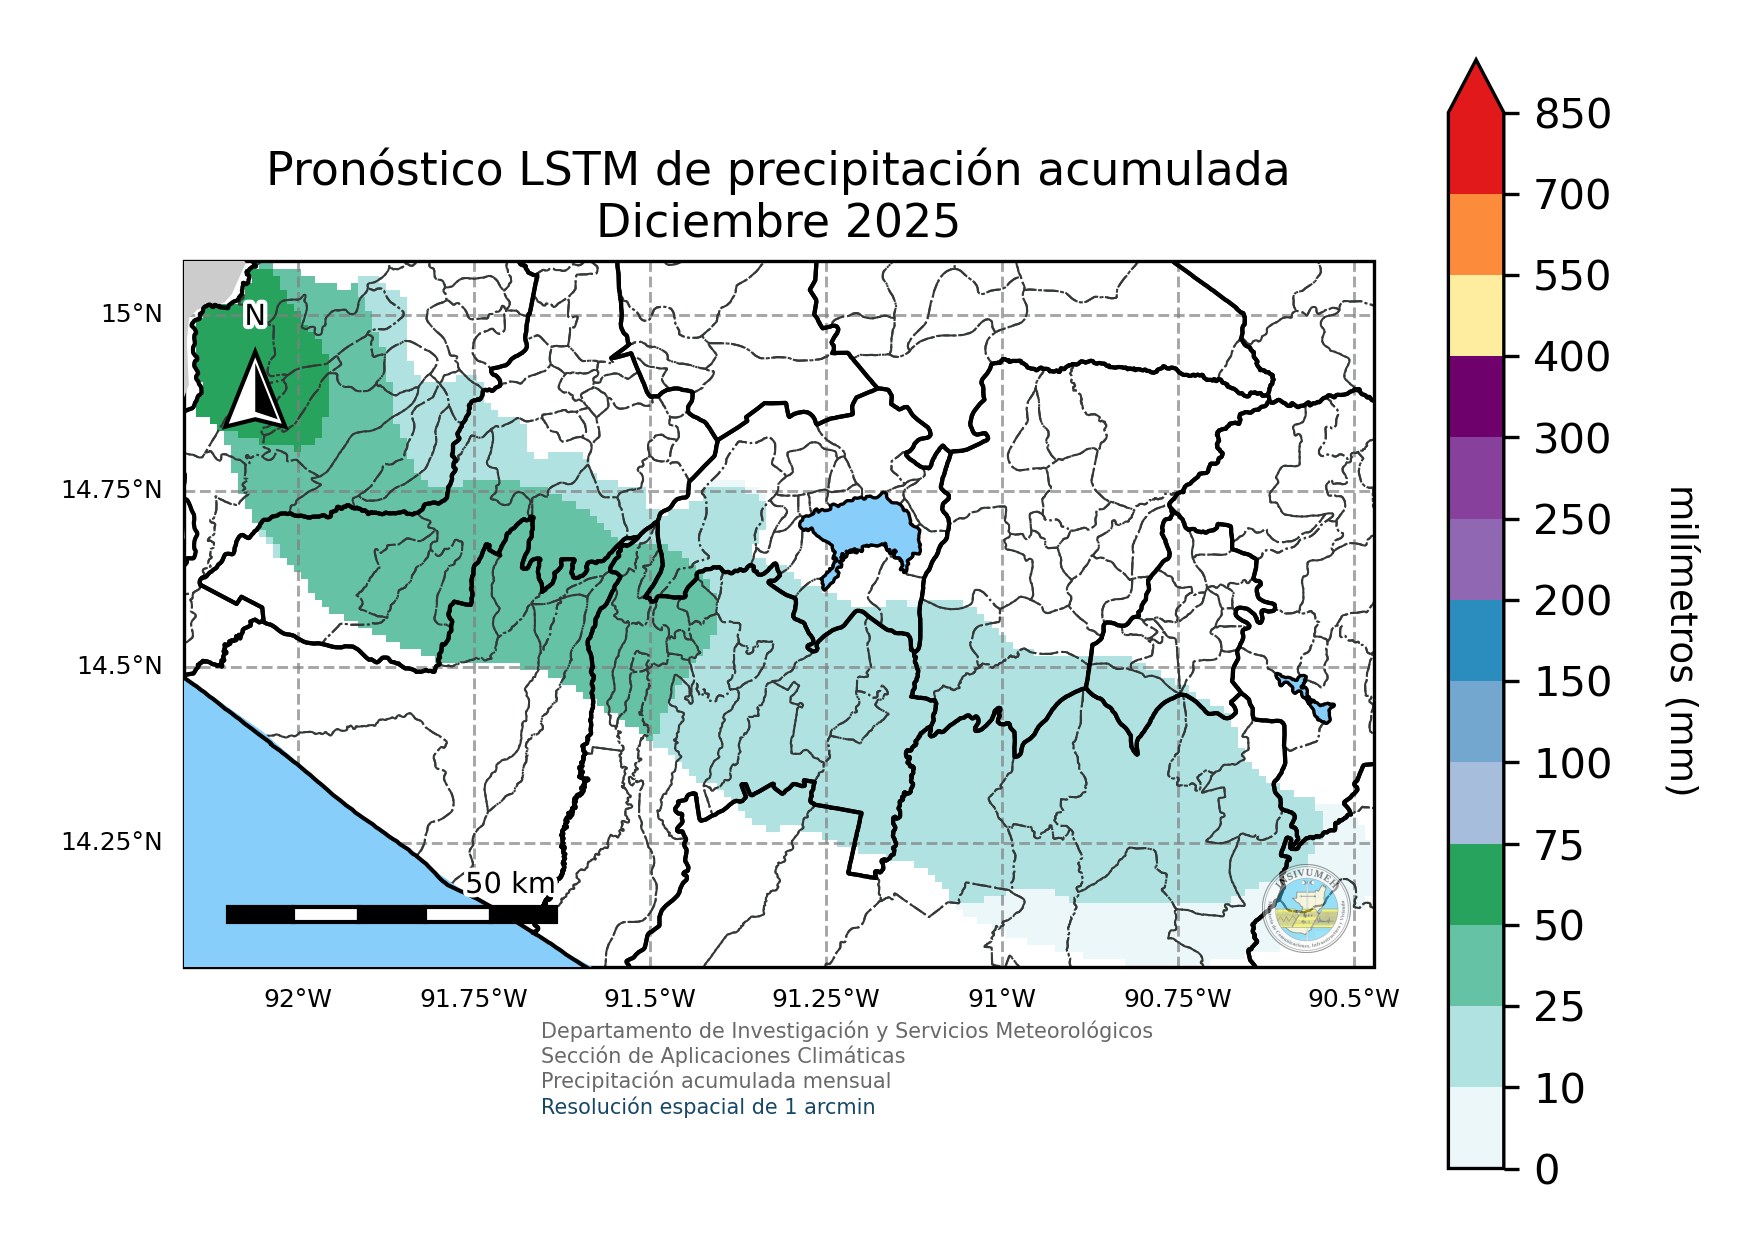
\includegraphics[width=\textwidth]{Informe/resultados/pronósticosLSTM/Pronóstico_LSTM_12_2025_Boca Costa_03.png}
	\end{subfigure}
	\hfill
	\begin{subfigure}[b]{0.45\textwidth}
		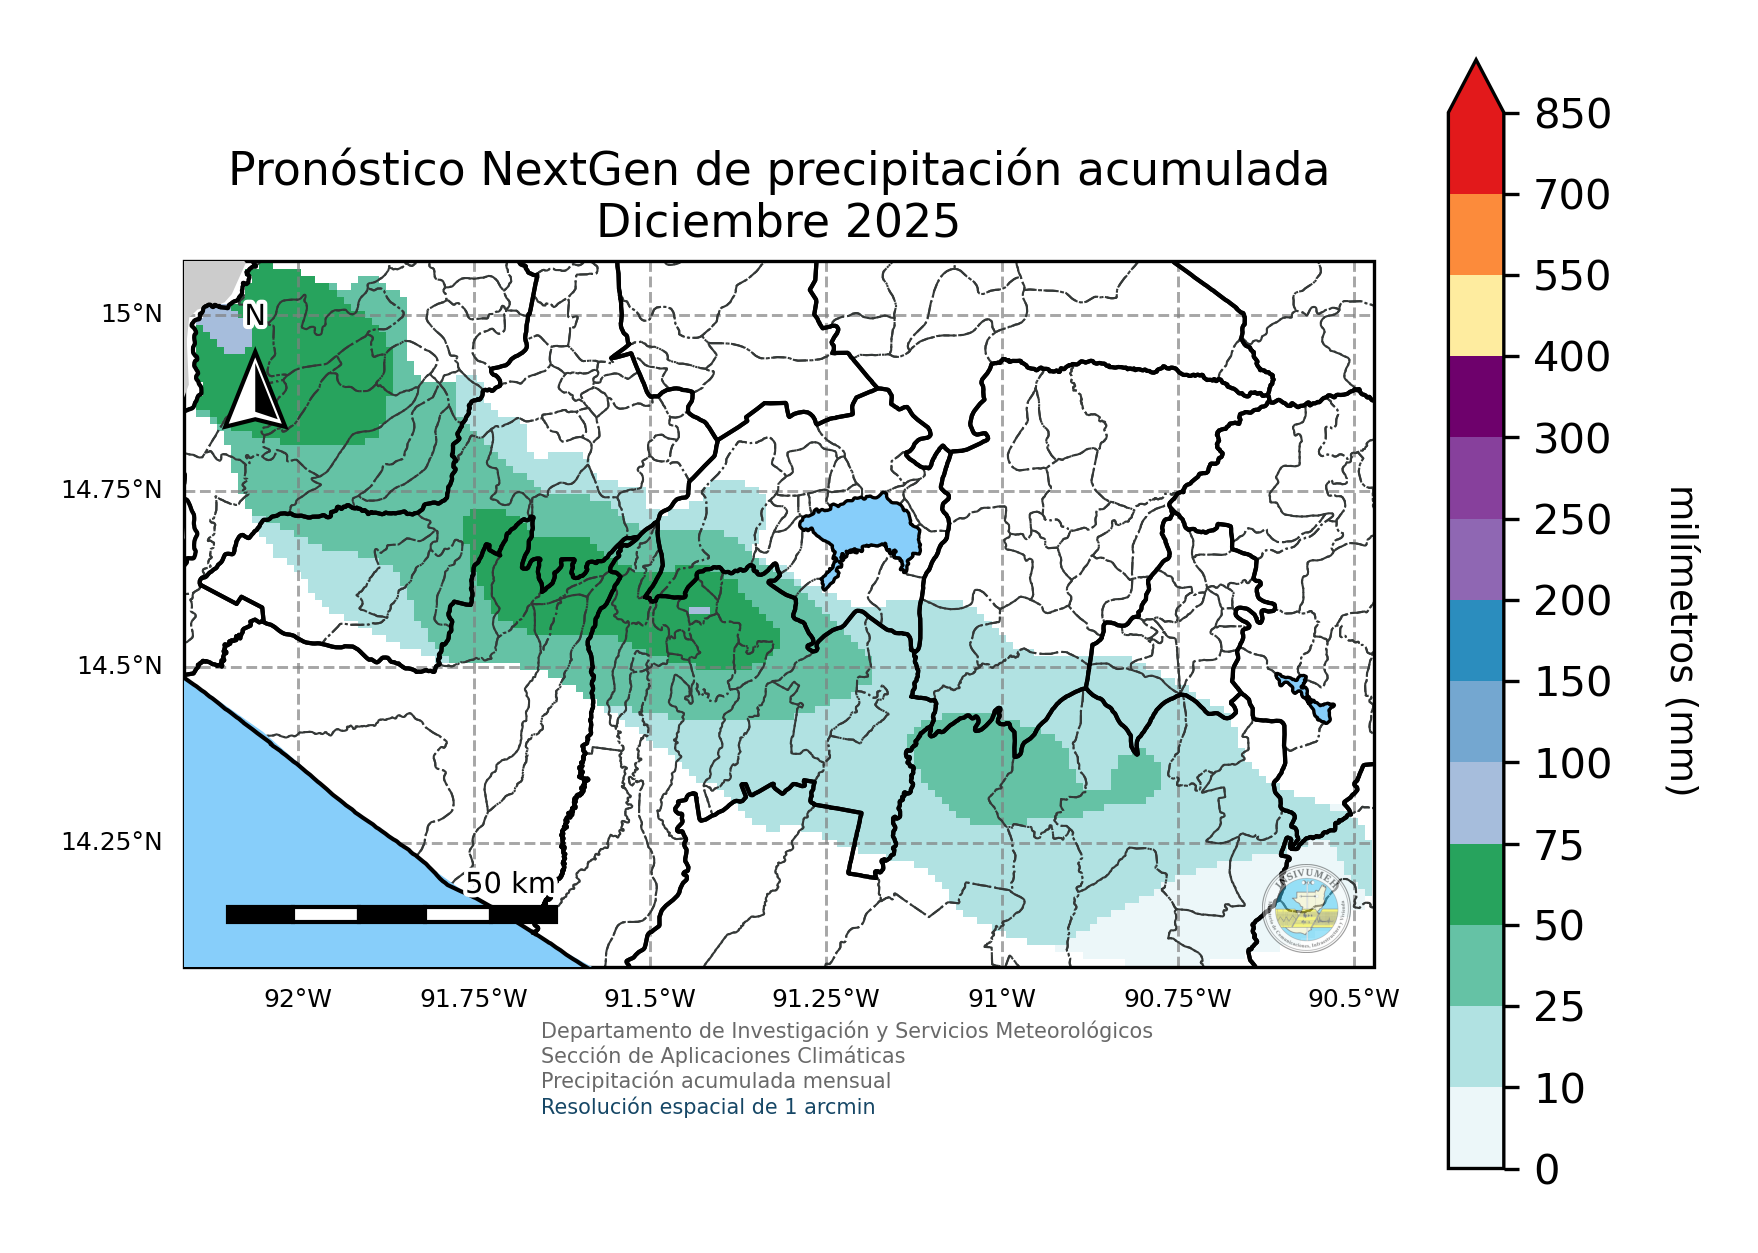
\includegraphics[width=\textwidth]{Informe/resultados/pronósticosNextGen/Pronóstico_NextGen_12_2025_Boca Costa_03.png}
	\end{subfigure}
	
	\vspace{-0.5em}
	
	\begin{subfigure}[b]{0.55\textwidth}
		\centering
		
\includegraphics[width=\textwidth]{Informe/resultados/precipitación/Precipitación_12_2025_Boca Costa_03.png}
	\end{subfigure}
	
\end{figure}

